\documentclass[12pt]{report}
\usepackage{changepage}
\usepackage{pdfpages}
\usepackage{float}
\usepackage[utf8]{inputenc}
\usepackage[norsk]{babel}
\usepackage[nottoc]{tocbibind}
\usepackage{tocloft}
\usepackage{lipsum}
%\usepackage[tmargin=2cm,bmargin=2.5cm,lmargin=2.5cm,rmargin=2cm]{geometry}
\usepackage{geometry}
\usepackage{hyperref}
\usepackage[round]{natbib}
\usepackage{graphicx}
\usepackage[parfill]{parskip}
\usepackage{setspace}
\usepackage{enumitem}
\usepackage[textsize=tiny]{todonotes}
\usepackage{listings}
\usepackage[title,titletoc,toc]{appendix}
\usepackage{titlesec}
\usepackage[acronym, toc]{glossaries} %Lager en merkelig S i starten av dokumentet
\usepackage{memhfixc}


\setcounter{secnumdepth}{5}


\lstset{language=SQL,morekeywords={PREFIX,,rdf,rdfs,master}}
%\renewcommand*{\glossarymark}[1]{}
\newcommand{\ot}[1]{\todo[color=green!40]{#1}}
\newcommand{\ob}{\todo[color=green!40]{Blabla}}

\setlist[description]{style=nextline}

%Fjerne første side, den inneholder en S fra \usepackage{glossaries}
\usepackage{atbegshi}
\AtBeginDocument{\AtBeginShipoutNext{\AtBeginShipoutDiscard}}

\lstset{
  numbers=left,
  stepnumber=1,    
  firstnumber=1,
  numberfirstline=true
}


%\usepackage{natbib}
%\bibliographystyle{abbrvnat}
%\setcitestyle{authoryear,open={((},close={))}}
\hypersetup{
    colorlinks,
    citecolor=black,
    filecolor=black,
    linkcolor=black,
    urlcolor=black
}
%\setlength{\arrayrulewidth}{1mm}
\renewcommand{\arraystretch}{1.5}
%\usepackage[backend=biber]{biblatex}
%\addbibresource{references.bib}
%\renewcommand{\bibname}{References}

% Leaders for chapter entries
%\renewcommand\cftchapdotsep{\cftdotsep}



\title{Semantisk webteknologi for klinisk farmasi: Evaluering av støttesystem ved legemiddelgjennomgang for pasienter med nedsatt nyrefunksjon}
\author{Håvard Moås, Espen Rise Halstensen, Frode Rennemo}


\spacing{1.5}
\setlist[itemize]{noitemsep, topsep=0pt}


\addto{\captionsnorsk}{\renewcommand*{\appendixname}{Vedlegg}}




\makenoidxglossaries
\newacronym{lib}{LiB}{Legemidler i bruk}
\newacronym{sparql}{SPARQL}{SPARQL Protocol and RDF Query Language}
\newacronym{nsd}{NSD}{Norsk senter for forskningsdata}
\newacronym{mvc}{MVC}{Model-View-Controller}
\newacronym{dron}{DrOn}{The Drug Ontology}
\newacronym{chebi}{ChEBI}{Chemical Entities of Biological Interest}
\newacronym{icd}{ICD}{International Statistical Classification of Diseases and Related Health Problems}
\newacronym{who}{WHO}{World Health Organization}
\newacronym{imm}{IMM}{Integrated Medicines Management}
\newacronym{limm}{LIMM}{Lund Integrated Medicines Management}
\newacronym{mvvm}{MVVM}{Model-view-viewmodel}



 




\begin{document}


\maketitle





\pagestyle{plain} 
\pagenumbering{roman}



%\frontmatter

\chapter*{Forord}
%\addcontentsline{toc}{kapittel}{\numberline{}Sammendrag}%

\chapter*{Sammendrag}


Legemiddelgjennomgang er en del av legemiddelhåndteringsprosessen ment å kvalitetssikre pasienters legemiddelbruk, ivareta effekt og sikkerhet samt forebygge skader. Ved legemiddelgjennomgang har helsepersonell behov for å finne relevant klinisk informasjon. Mangel på søkeferdigheter og økende volum av informasjon fører til at søken etter informasjon er en tidkrevende og problematisk prosess. Manglende funn av relevant informasjon kan føre til at legemiddelgjennomgangen tar lengre tid og være av lavere kvalitet enn den kunne ha vært. Semantisk webteknologi kan være til støtte ved å gjenbruke data på tvers av applikasjoner, samt aggregere og kombinere data. 

Målet med masteroppgaven var å bruke semantisk webteknologi for å støtte opp om legemiddelgjennomgangsprosessen. Forskningsspørsmålet som ble besvart var følgende:
 \textit{Kan et system  basert på semantisk web-teknolgi hjelpe farmasøyter til å gjøre legemiddelgjennomgang slik at den blir mer presis, raskere gjennomført og lærerik.}

En prototype der legemiddelgjennomgang utføres elektronisk ble utviklet. Prototypen ga brukeren forslag til tiltak der nedsatt nyrefunksjon påvirket pasienters opptak av legemidler. Et eksperiment med bruk av prototypen ble utført av for å besvare forskningsspørsmålet. Eksperimentet sammenlignet utførelsen av legemiddelgjennomgang med og uten forslag til tiltak. Legemiddelgjennomgangen ble utført av kliniske farmasøyter.  

Konklusjonen av eksperimentet var at forslag til tiltak ga mer presis legemiddelgjennomgang og læringsutbytte enn uten forslag. Tidsbruken ble lengre ved bruk av støtten.   

%.\ot{Er dette for detaljert/unødvendig?} En nettside fungerte som brukergrensesnitt for tilhørende kunnskapsbase utviklet med bruk av semantiske webteknologier.
%Legemiddelbruk er et viktig tiltak i helsevesenet, men er uten samlet kontroll og ofte mindre koordinert mellom ulike institusjoner. Suboptimal koordinering mellom helseinstitusjoner kan føre til utilsiktede hendelser som konsekvens av legemiddelrelaterte problemer. En slik systematisk gjennomgang av en pasients legemidler kan eliminere noen av problemene knyttet til et fragmentert helsevesen, og forbedre legemiddelbehandlingen. 
%\addcontentsline{toc}{kapittel}{\numberline{}Sammendrag}%
\newpage

\tableofcontents

\chapter*{Ordliste}
%\begin{description}
%\item[<ord>]
% <beskrivelse>
%\end{description}

\begin{description}
\item[Legemiddelgjennomgang]
 er en systematisk vurdering av pasientens legemiddelbruk. \citep{Legemiddelverket_LMG}. 
\end{description}

\begin{description}
\item[Legemiddelsamstemming]
er å lage en liste over alle legemidler pasienten bruker. Legemiddelinformasjonen blir hentet fra journaler, intervjuer eller samtaler med fastlege.
\end{description}

\begin{description}
\item[Farmakogenetikk]
er læren om hvordan gener påvirker kroppens opptak av legemidler.
\end{description}


\begin{description}
\item[Legemidler i bruk]
er en liste over legemidler en pasient bruker. Denne listen blir laget under en legemiddelsamstemming.
\end{description}


\begin{description}
\item[Bivirkning]
er en sideeffekt man kan få av et legemiddel eller en annen behandling.
\end{description}

\begin{description}
\item [Interaksjon]
er når to eller flere medisiner påvirker hverandre.
\end{description}

\addcontentsline{toc}{chapter}{Ordliste}


%Forkortelser

\printnoidxglossary[title=Forkortelser,type=\acronymtype]


\renewcommand{\listtablename}{Tabelliste}
\listoftables

\renewcommand{\listfigurename}{Figurliste}
\listoffigures


\chapter{Innledning}
\setcounter{page}{0}
\pagenumbering{arabic}
Utførelsen av legemiddelgjennomgang er et svært viktig tiltak for å bidra til redusering av legemiddelrelaterte problemer. ''Legemiddelrelaterte problemer forekommer hyppig og påfører pasientene betydelig sykelighet og i noen tilfeller død, samt økte utgifter for samfunnet.'' \citep{norske_legeforening}. 

Tittelen på masteroppgaven er: ''Semantisk webteknologi for klinisk farmasi: Evaluering av støttesystem ved legemiddelgjennomgang for pasienter med nedsatt nyrefunksjon''. Med \textit{støttesystem} mener vi et system som skal bidra med forslag til tiltak for å redusere legemiddelrelaterte problem. Systemet er basert på \textit{semantisk webteknologi}. Med semantisk webteknologi åpnet det seg muligheter for delbarhet og gjenbruk. Formålet med å evaluere støttesystemet var å identifisere om tiltakene gir en effekt under \textit{legemiddelgjennomgang}. \textit{Kliniske farmasøyter} er farmasøyter med tilleggsutdanning som gjør at de sitter med kompetanse til å kvalitetssikre legemiddelbruk. Dette er en yrkesgruppe som støttesystemet vil kunne være et hjelpemiddel for.


Dette kapittelet utgreier mål, motivasjon, forskningsspørsmål og begrensninger for oppgaven.

\section{Motivasjon}
\subsection{Feil i legemiddelhåndteringsprosessen}
Legemiddelbruk kan være skadelig, og legemiddelrelaterte problemer er svært utbredt i Norge. Over 1000 norske pasienter dør hvert år som følge av bivirkninger og uheldig bruk av legemidler\citep{apotekforeningen_fakta_om_legemiddelbruk}. Feil legemiddelbruk trenger ikke å være direkte skadelig, men det er mulig at bruk av andre legemidler fører til en bedre legemiddelbehandling.  

Mindre optimal legemiddelbruk kan det være flere årsaker til. Legemiddelbruk er uten samlet kontroll og ofte mindre koordinert mellom ulike institusjoner. Dårlig koordinering mellom helseinstitusjoner kan føre til utilsiktede hendelser som konsekvens av legemiddelrelaterte problemer. Videre kan multifarmasi være en årsak til mindre optimal legemiddelbruk. Pasienter med flere kroniske sykdommer, og som derfor tar flere legemidler samtidig, har økt\citep{Uijen_Lisdonk}. Ved multifarmasi øker sannsynligheten for dårligere etterlevelse \citep{Ulfvarson}. Med etterlevelse menes det å ta legemidler som forskrevet.

En systematisk gjennomgang av en pasients legemidler kan eliminere konsekvensene knyttet til et fragmentert helsevesen, og forbedre legemiddelbehandlingen. En norsk studie ble det observert at 81\% av pasientene hadde minst et legemiddelrelatert problem.\citep{81prosent_LRP} For å bedre legemiddelbehandlingen ble det i 2004 foreslått pilotprosjekter for legemiddelgjennomganger. \citep{Helsedirektoratet_veileder_LMG} I 2014 ble det økt satsning på å få kliniske farmasøyter på avdelingene ved St. Olavs. I dag er det ca. 10 årsverk med kliniske farmasøyter som jobber ved St. Olavs hospital i Trondheim og i løpet av året skal det ansettes 5 til.


\subsection{Informasjonssøking er problematisk}
Flere studier har vist at klinisk helsepersonell har et stort behov for å finne relevant klinisk informasjon, og at søken etter dette er problematisk \citep{Information_Needs_Information_Seeking_PHC}\citep{Information_Needs_Being_Met}\citep{IR_Patterns_Surgeons}. Studiene peker både på mangel av relevant informasjon men også mangel på søkeferdigheter som årsak. I de senere tiår har volumet av informasjon økt betraktelig, også innenfor helsesektoren. Søking og filtrering av relevant informasjon blir krevende når volumet og antall kilder øker. Videre har dette ført til økning av tvilsom informasjon og verktøy ment brukt innenfor helsesektoren \citep{Rating_Health_Information}. Ukritisk bruk av informasjon og verktøy på internett kan være skadelig både for pasienter og helsepersonell. 

Etter samtaler med kliniske farmasøyter og forskere i dette feltet, har det kommet frem at det er ingen enighet om hvilke informasjonskilder til legemidler man benytter seg av. Med andre ord vil valg av informasjonskilder gå på personlige preferanser. Informasjonskildene i bruk er mange og det er et stort spenn i innhold, fokus og målgruppe.

\subsection{Semantisk webteknologi gir nye muligheter}
Semantisk web er en utvidelse av den tradisjonelle verdensveven der informasjonen er gitt en veldefinert mening. Ved å ha standardiserte formater og utvekslingsprotokoller, kan kunnskap bli delt og gjenbrukt på tvers av applikasjoner.
Dette kan igjen tilrettelegge for resonnering med kunnskapspresentasjoner. 

\citet{monitor_bipolar_semanticweb} og \citet{semanticweb_clinical_guideline} har sett nytte i å bruke semantiske teknologier innenfor helse-og biovitenskap. Her er det store problemer med heterogene data som er spredt over ulike domener. Samtidig vokser datamengden. Forskere og andre må kunne foreta spørringer som går på tvers av disse for å kunne ta kritiske avgjørelser. Bruk av semantiske teknologier kan redusere kostnadene ved en slik integrasjon av datakilder. W3C opprettet Semantic Web for Health Care and Life Sciences Interest Group for å utvikle, støtte samt være en pådriver for bruken av semantiske teknologier i helse-og biovitenskap\citep{W3C_HCLSIG}.


\section{Forskningsspørsmål}
\label{innled:forskningsporsmal}
%Å sette seg inn i et komplekst domene som helsesektoren, har vært en lang og krevende prosess\ot{Vær konsise og direkte. Dette er bortforklaringer.}. Siden vi hadde begrenset kunnskap om problemområdet til å begynne med, var forskningsspørsmålene våre vage og omfattende. Disse kunne ikke besvares uten ytterligere konkretisering. Med tiden fikk vi en økt forståelse for domenet, som førte til mer og mer konkrete forskningsspørsmål samt ytterligere innsnevringer. 

%I starten av masteroppgaven var målet å utvikle en komplett kunnskapspresentasjon med tilhørende grensesnitt, altså et ferdigutviklet system. Etterhvert forsto vi at vi ikke hadde tid til å ferdigstille et system samt gjennomføre et forsøk. På grunnlag av dette ble problemområdet innskrenket til å fokusere på pasienter med nedsatt nyrefunksjon, men samtidig beholde forskningsspørsmålene vi hadde utviklet underveis. Dette ga oss muligheten til å utvikle et Proof-of-concept, som lar oss demonstrere konseptet\ot{løsning, idé - konsept er et konsulentord}, designmuligheter og samtidig besvare forskningsspørsmålene. Selv om systemutvikling ikke er forskning i seg selv, så vi det som nødvendig å lage et system for å gjøre et forsøk så virkelighetsnært som mulig.\ot{prototyp for å teste idé/teori = forskning og del av metoden!} 

Overordnet forskningsspørsmål:

\begin{enumerate}
    \item Kan et system  basert på semantisk web-teknolgi hjelpe farmasøyter til å gjøre legemiddelgjennomgang slik at den blir 
    \begin{itemize}
        \item mer presis,
        \item raskere gjennomført
        \item og lærerik.
    \end{itemize}
\end{enumerate}

Som del av dette må vi også besvare følgende underordnede spørsmål:
\begin{enumerate}
\setcounter{enumi}{1}
\item Hvordan kan vi gjennomføre et eksperiment for å besvare spørsmål 1? Hvilke forskningsmetoder passer vårt behov og våre ressurser?
\item Hvilke kunnskapskilder og hva slags type teknologi er relevant og tilstrekkelig?
\item Hva betyr, og hvordan måles, presisjon, effektivitet og læreeffekt av legemiddelgjennomgang?
\end{enumerate}
\section{Utvikling av prototype}
Vi utviklet en prototype i form av en webapplikasjon, der brukeren foretok legemiddelgjennomgang basert på to kasuistikker. Formålet med prototypen var å bruke det i et eksperiment for å besvare forskningsspørsmålet. I eksperimentet sammenlignet vi bruk av prototypen med og uten forslag til tiltak tilgjengelig. Forslag til tiltak ble gitt der nedsatt nyrefunksjon påvirket pasientens opptak av legemidler\ot{Må vi argumentere for hvorfor vi fokuserer på nedsatt nyrefunksjon? }. Nedsatt nyrefunksjoner er et av punktene det er viktig å ta hensyn til under en legemiddelgjennomgang\citep{Helsedirektoratet_veileder_LMG}. 



%For å kunne besvare forskningsspørsmålet ble en prototype utviklet. Prototypen var en webapplikasjon der legemiddelgjennomgang ble foretatt elektronisk. I denne masteroppgaven har vi fokusert på den delen av legemiddelgjennomgang som går på nyrefunksjon. Nedsatt nyrefunksjon er en av de punktene det er viktig å ta hensyn til under en legemiddelgjennomgang\citep{Helsedirektoratet_veileder_LMG}. Vi har laget et system vi kan bruke som et verktøy for å få svar på forskningsspørsmålene. Prototypen tar hensyn til legemidler i bruk fra kasuistikkene vi har lagt inn og gir anbefalinger til bruker ut i fra den aktuelle nyrefunksjonen til pasienten. Prototypen skal brukes til et forsøk der kliniske farmasøyter gjennomfører legemiddelgjennomgang elektronisk. 

\section{Begrensninger\ot{skal vi ha dette?}}
Her presenteres begrensninger valgt for masteroppgaven.
\subsection{Personvern}
Vi har ikke sett lagring av reelle persondata som nødvendig hverken i utviklingen av prototypen eller i gjennomføring av forsøk. På dette viset har vi unngått potensielle problemstillinger knyttet til personvern. Det er likevel svært viktig at et ferdigutviklet system tar hensyn til problemstillinger relatert til personvern. Problemstillinger knyttet til personvern er diskutert i \ref{Personvern}.

 


\chapter{Legemiddelgjennomgang}
Legemiddelgjennomgang er et tiltak som er iverksatt for å sikre pasientens legemiddelbruk. Begrepet legemiddelgjennomgang er nødvendig for å forstå forskningspørsmålet jf. delkapittel \ref{innled:forskningsporsmal}. Dette kapitellet vil ta for seg det nødvendigste om legemiddelgjennomgang samt hvordan det er implementert i Midt-Norge.

\section{Hva er legemiddelgjennomgang}
Legemiddelgjennomgang er en systematisk fremgangsmåte for å kvalitetsikre pasientens legemiddelbruk, ivareta effekt og sikkerhet samt forebygge skader. En legemiddlegjennomgang iverksettes når det er endringer i pasientens tilstand eller omsorgstilbud og skal gjøres årlig for pasienter som går på flere enn tre legemidler. Gjennomgangen utføres av behandlende lege alene eller sammen med farmasøyt og/eller sykepleier. Det er også mulighet for at pasienten eller pårørende kan delta i gjennomgangen. \citep{Helsedirektoratet_veileder_LMG}.

\section{Bakgrunn}
For å bedre legemiddelbehandlingen i Norge ble det i Stortingsmelding nr. 18 (2004-2005) foreslått flere ulike tiltak fra Helse- og omsorgsorgsdepartamentet \citep{Stortingsmelding_nr18}. Et av disse tiltakene var pilotprosjekter for legemiddelgjennomganger. Dette har ført til at Helsedirektoratet har i flere år gitt tilskudd til prosjekter knyttet til legemiddelgjennomgang. Disse prosjektene foregikk på sykehus, i syke- og aldershjem, i hjemmesykepleien og apotek.

\section{Målsetting}
Studier viser at legemidler brukes uhensiktsmessig på sykehus, i sykehjem og hos pasienter forøvrig. Avhengig av hvilke kriterier pasientene har, er det rapportert om feilforskrivning av legemidler i 10 - 25 prosent av forskrivningene \citep{NORGEP} \citep{Elderly_patients_in_general_practice} \citep{Inappropriate_Prescribing_for_Elderly_Americans}. Om lag 10 prosent av innleggelse av eldre på medisinsk avdeling skyldes av legemiddelrelaterte problemer. 

Målet med legemiddelgjennomgang er at den enkelte pasient oppnår god effekt av legemidlene pasienten går på. Med en slik systematisk gjennomgang vil legemidlene kunne endres ved seponering, dosejustering eller at nye legemidler forskrives for å ytterligere forbedre legemiddelbehandlingen.

\section{Fremgangsmåte}
For å sikre den enkelte pasientens legemiddelbruk er det viktig med en god fremgangsmåte for legemiddelgjennomgangen. Fremgangsmåten avhenger av pasientgruppe og helsepersonell og må utvikles på hvert enkelt behandlingsted. I figur \ref{fig:lmgfremgangsmate} kan vi se en skjematisk fremstilling av Helsedirektoratets forslag til fremgangsmåte. Fremgangsmåten og annen informasjon om legemiddelgjennomgang finner vi i deres veileder. \citep{Helsedirektoratet_veileder_LMG}

\begin{figure}[H]
\centering
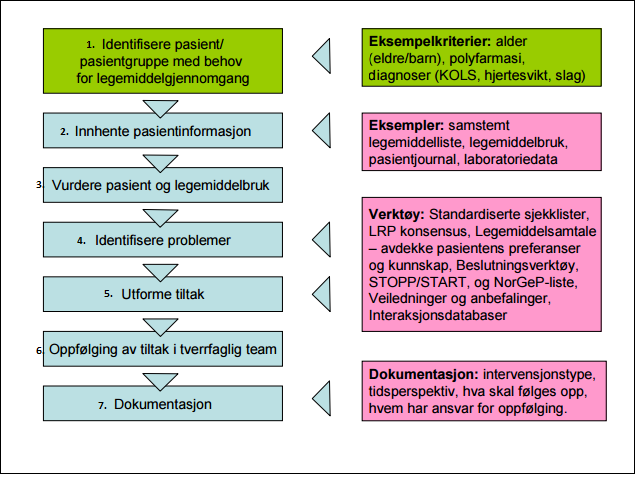
\includegraphics{images/skjematisk_fremgangsmaate_lmg.png}
\caption{Skjematisk fremgangsmåte for legemiddelgjennomgang}
\label{fig:lmgfremgangsmate}
\end{figure}

Hvert steg av fremgangsmåten er viktig for pasientens legemiddelbruk sikkerhet. Under ønsker vi å se nærmere på hva stegene innebærer.

\begin{enumerate}
\item \textbf{Identifisere pasient/pasientgruppe med behov for legemiddelgjennomgang}\\ 
Identifisering av pasient/pasientgruppen er utslagsgivende for når og hvor ofte det skal gjennomføres legemiddelgjennomgang.
Ved denne fasen vil pasientens alder, sykdomstilstand og behov bli identifisert.
\item 
\textbf{Innhenting av nødvendig pasientinformasjon}\\ 
Dette er et viktig grunnlag for aktuelle diagnoser og gir indikasjon for legemiddelbehandling. Her må det være gjennomført grundig og bred klinisk undersøkelse med supplerende informasjon. 

\begin{description}
\item[Legemiddelsamstemming]
Informasjon om den enkelte pasients legemiddelbruk er en viktig forutsetning for en meningsfull legemiddelgjennomgang.
Før en legemiddelgjennomgang utføres må det hentes inn en oppdatert oversikt over de legemiddlene en pasient bruker. Dette kalles en samstemt legemiddelliste og skal inkludere informasjon fra flest mulig av de aktuelle og tilgjengelige kildene. Dersom det er avvik mellom de forskjellige informasjonskildene, må dette komme frem i listen og avklares før eller under en legemiddelgjennomgang. Denne listen skal følge med pasienten ved et eventuelt omsorgsskifte. Prosedyrer for legemiddelsamstemming skal etableres ved de lokale institusjoner.
\end{description}

\begin{description}
\item[Kommunikasjon med pasient/pårørende] 
En annen informasjonskilde som er viktig for legemiddelgjennomgang er pasientens egen forståelse og motivasjon. Dette er for å sikre best mulig etterlevelse av legemiddelbehandlingen. For enkelte pasientgrupper er det viktig med dialog med pårørende. For pasienten kan informasjonen som blir utvekslet under en legemiddelgjennomgang være en mulig til å kunne medvirke i egen behandling. Dette kan bidra til riktigere bruk og gi pasienten mulig til å selv kjenne igjen legemiddelrelaterte problemer.
\end{description}

Det finnes også annen informasjon som er viktig for legemiddelgjennomgangen. Informasjon som bruk av naturmidler, kosttilskudd og ikke-reseptbelagte legemiddler bør innhentes. Det kan også være aktuelt å innhente informasjon om tidligere allergier og signifikante bivirkninger av legemidlene som skal brukes/har vært brukt.

\item \textbf{Vurdere pasient og legemiddelbruk}\\
For å støtte legemiddelvalg med bakgrunn i legemiddelgjennomgang må det benyttes beslutningsstøtteverktøy, sjekklister, interaksjonsdatabaser og liknende.\\
Under er ei typisk liste over hvilken informasjon som trengs om pasient og legemiddelbruk:
\begin{itemize}
\item Hvilke indikasjoner har pasienten?
\item Får pasienten behandling for alle behandlingstrengende indikasjoner?
\item Har pasienten indikasjon for alle legemidlene som er forskrevet?
\item Kan noen av indikasjonene skyldes bivirkninger og/eller interaksjoner forårsaket av andre legemidler?
\item Er behandlingen i samsvar med behandlingsretningslinjer?
\item Avklar pasientens evne og vilje til å ta legemidler og ev. håndtere disse selv 
\end{itemize}

\item 
\textbf{Identifisere legemiddelrelaterte problemer}\\
 Med stadig flere legemidler og flere pasienter som bruker legemidler, gjerne flere samtidig, øker risiko for bivirkninger og legemiddelinteraksjoner, og gjennomføring av medisineringen blir vanskeligere. \citep{DNL_klassifisering_av_legemiddelrelaterte_problemer} \\

Under er legemiddelrelaterte problemer tematisk satt opp. Ut fra spørsmålene under hvert område vurderes det om pasienten har et aktuelt eller et potensielt legemiddelrelatert problem.\citep{Helsedirektoratet_veileder_LMG}

\begin{description}
\item[Legemiddelvalg:]
    \begin{itemize}
    \item[]
    \item Er det fortsatt indikasjon for legemidlet?
  \item Har pasienten tilstrekkelig effekt av legemidlet?
  \item Bruker pasient kurlegemiddel
  \item Mangler pasienten legemiddel for diagnoser/ tilstand? \textit{For eksempel: Jern, vitamin B12, folsyre, protonpumpehemmere,analgetika, antidepressiva og antikoagulantia}
  \item Er legemidlet hensiktsmessig for denne pasienten? \textit{ Bruk beslutningsstøtte-verktøy og oppslagsverktøy. Kontroller at pasienten ikke er satt på legemiddel som er registrert under CAVE/legemiddel-følsomhet.}
  \item Har pasienten ubehandlet indikasjon/tilstand (manglerlegemiddel)?
\end{itemize}

\item[Dosering:]
\begin{itemize}
\item[]
\item Er dosen, doserings-tidspunkt og administrasjon i samsvar med pasientens nåværende situasjon?
\item Kontroller om legemiddel og doser er tilpasset den enkelte pasient med \textit{hensyn til bl.a. nyrefunksjon, leverfunksjon, kontraindikasjoner og andre sykdommer.}
\end{itemize}

\item[Bivirkning:]
\begin{itemize}
\item[]
\item Tolererer pasienten legemidlet? 
\item Har pasienten bivirkninger?
\item Er pasienten/ pårørende kjent med hva hun/han selv må være oppmerksom på når det gjelder administrering, kost, alkohol, interaksjoner med ikke-registrerte legemidler (naturpreparater).
\item Kontroller om legemiddel kan være årsak til bivirkninger, symptom eller forandrede labverdier
\end{itemize}

\item[Interaksjon:]
\begin{itemize}
\item[]
\item Er det interaksjoner av klinisk betydning mellom legemiddellegemiddel eller mellom legemiddel-sykdom eller legemiddel-mat/helsekost og liknende?
\end{itemize}

\item[Avvikende legemiddelbruk:]
\begin{itemize}
\item[]
\item Håndterer og bruker pasienten legemiddelet slik angitt i kurve/journal, og dersom ikke – hvordan gjør/bruker pasienten det? 
\item Er det praktiske håndteringsproblem? 
\small
\begin{itemize}
\item Kontroller om det er behov for knusing av tabletter/ åpning av kapsler pga. svelgeproblemer/ sonde.
\item Hvis pasienten bruker øyedråper, inhalatorer eller lignende 
\item Sjekk teknikk
\end{itemize}
\end{itemize}

\item[Manglende monitorering:]
\begin{itemize}
\item[]
\item Håndterer og bruker pasienten legemiddelet slik angitt i kurve/journal, og dersom ikke – hvordan gjør/bruker pasienten det? 
\item Er det praktiske håndteringsproblem? 
\small
\begin{itemize}
\item Kontroller om det er behov for knusing av tabletter/ åpning av kapsler pga. svelgeproblemer/ sonde.
\item Hvis pasienten bruker øyedråper, inhalatorer eller lignende 
\item Sjekk teknikk
\end{itemize}
\end{itemize}

\item[Andre problemstillinger:]
\begin{itemize}
\item[]
\begin{itemize}
\item[]
\item Er det eventuelle andre momenter å diskutere når det gjelder legemiddelregimet? 
\item Avvik i legemiddelliste.
\end{itemize}
\end{itemize}
\end{description}

\item \textbf{Utforme forslag til tiltak}\\
En legemiddelgjennomgang kan føre frem synlige behov for justing av legemiddelterapien.Endringene/tiltakene utformes med bakgrunn i de avdekkede legemiddelrelaterte problemene. Hvis det skulle oppstå uenigheter i det tverrfaglige teamet er det legen som tar den endelige avgjørelsen.

\item \textbf{Oppfølging av foreslåtte tiltak i tverrfaglige team
}\\
I et tverrfaglig team vil forskjellig helsepersonell ha forskjellige roller, og det er opp til det enkelte helseforetak å organisere seg på best mulig måte. Uavhengig av denne organiseringen er det behandlende lege som tar den endelige avgjørelsen. 

Oppgavene som er knyttet til legemiddelgjennomgangen er avhengig av behandlingstedet, men under er en liste over særlige aktuelle tema:

\begin{itemize}
\item Gi faglig rådgivning om legemiddelbruk: blant annet interaksjoner, alternative legemidler, dosering, potensielle bivikrninger
\item Koordinere legemiddelgjennomgangen
\item Kartlegge pasientens mentale funksjon, bla. i dagliglivets aktiviteter. Dette er særlig aktuelt ved institusjoner og i hjemmebasert omsorg
\item Registrere pasientens evne til å etterleve legemiddlebehandlingen
\item Registere om pasienten trenger bistand til endringer
\item Observere pasienten
\item Generell observasjon av pasient i etterkant av legemiddelendringer
\item Dokumentere/melde dette tilbake til behandlende lege
\item Vurdere ikke-medikamentell behandling
\end{itemize}
Ved foretak hvor tverrfaglige team ikke lar seg enkelt etableres, vil det være naturlig for behandlende lege og forhøre seg med andre leger hvis pasientens legemiddelbilde er komplisert.

\item \textbf{Dokumentasjon av gjennomgangen} \\
Dokumentasjon av legemiddelgjennomgangen skal inneholde:
\begin{itemize}
\item Hvilke legemiddelrelaterte problemer er avdekket
\item Hva krever tiltak og/eller oppfølging
\item Til hvilket tidspunkt skal tiltakene utføres, og av hvem
\end{itemize}
Dersom det utføres ekstra utredning i forbindelse med gjennomgangen (litteratursøk, omfattende interaksjonsøk og liknende) må det vurderes om dette skal registreres i elektronisk pasientjournal.
\end{enumerate}




%\begin{itemize}
%\item Hva er legemiddelgjennomgang.\\
%Sikre bruken av legemiddler og forebygge skader. \\
%Se kapittel 2.2 i [3], her er det mye som kan brukes.
%\item Hvorfor gjennomføres legemiddelgjennomgang.

%\item Hvordan utføres en legemiddelgjennomgang i dag.
%\item Kan nevne LMS (Legemiddelsamstemning) og LIB (Legemiddler i bruk). \\
%Legemiddelgjennomgang krever at en samstemt legemiddel liste er tilgjengelig.
%\end{itemize}
\section{Legemiddelgjennomgang i Midt-Norge}
Prosessen med å ha tjenester som kan sjekke legemiddeldoseringer og legemiddelrelaterte problemer hos pasienter i spesialhelsetjenesten startet for tjue år siden i Midt-Norge. Kliniske farmasøyter ble sendt ut på post for å utfylle noe av jobben for sykepleiere og leger. I Midt-Norge fungerer kliniske farmasøyter som en tjeneste som kan benyttes på forskjellige poster hvor det er behov for legemiddelsamtstemming, legemiddelgjennomgang og andre legemiddelhåndteringer. 

\subsection{IMM-modellen}
På 2000-tallet ble \gls{imm} utviklet ved Queens University of Belfast i Nord-Irland. Dette er en modell for utøving av klinisk farmasi. Målet med modellen er å oppnå maksimal helse gjennom optimal bruk av legemidler.  \gls{imm} beskriver en sømløs prosess og integrerer behandlingsnivåene i hverandre i tillegg til
å integrere farmasøyten i det tverrfaglige behandlingsteamet. 

Det er systematisk måte å jobbe på for å :
\begin{itemize}
\item å kvalitetessikre pasientens legemiddelliste
\item å individualisere og optimalisere legemiddelbehandlingen for pasienter
\item å sikre informasjonsoverføring til andre omsorgsnivåer (sykehjem, fastlege, hjemmesykepleier)
\item å involverer pasienten til å forstå legemiddelbehandlingen
\end{itemize}
I Lund i Sverige ble IMM-modellen videreutviklet og tilpasset svenske forhold og ble dermed til \gls{limm}. \gls{limm} har strukturerte og forskningsbaserte prosedyrer og verktøy inkludert faglige dokumenter til å vurdere den enkelte pasientens legemiddelbehandling. \gls{limm} inneholder også spesifikke kompetansekrav og standardiserte opplæringsprosedyrer. 

I 2010 ble \gls{limm} utviklet i Midt-Norge med utgangspunkt i den svenske \gls{limm}. \gls{imm} i Midt-Norge har som mål å forbedre legemiddelbehandlingen til den enkelte pasienten og har fokus på tverrfaglig samarbeid. Den kliniske farmasøyten har som oppgave å identifisere, løse og forebygge legemiddelrelaterte problemer og kommer med forslag og innspill til legen for å kvalitetssikre legemiddelbehandlingen. Modellen involverer moduler til bruk ved innleggelse, under sykehusopphold og ved utskrivning. I figur \ref{fig:imm}  blir det illustrert hva som gjøres under hver hendelse, hvor legemiddelgjennomgang er en del av sykehusoppholdet.
\\\citep{IMM_i_midtnorge}

\begin{figure}[H]
\centering
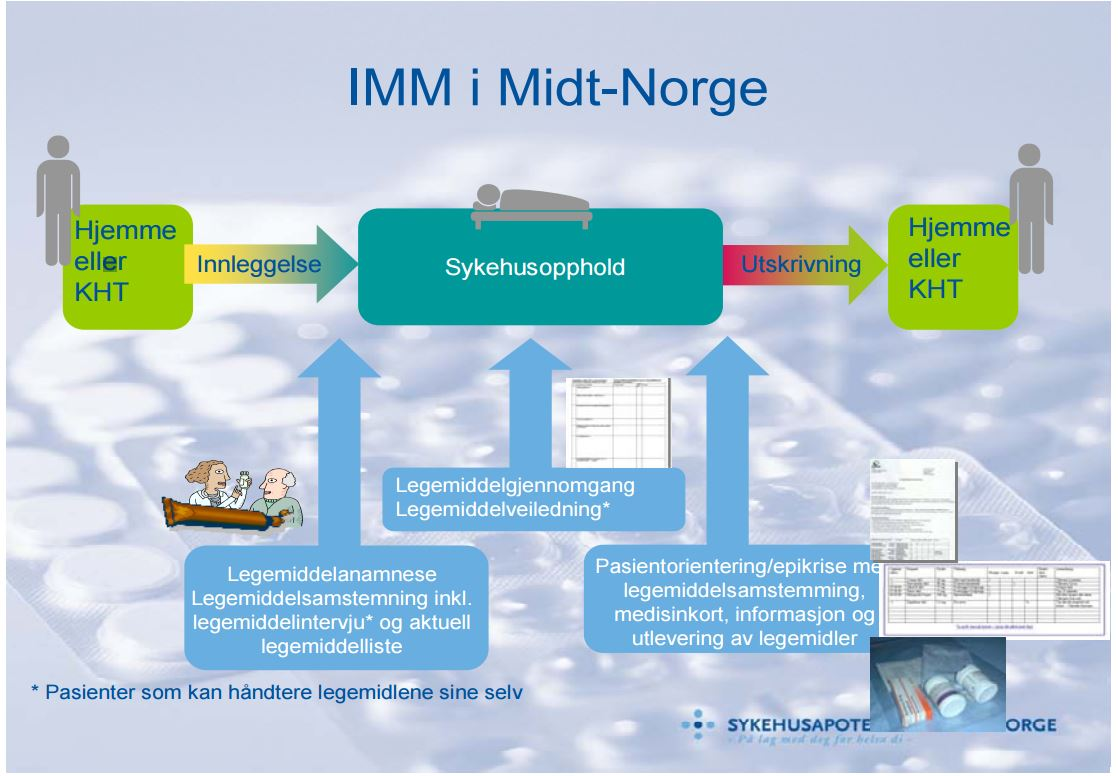
\includegraphics[width= 12cm]{images/IMM_I_MIDT_NORGE.JPG}
\caption{IMM i Midt-Norge}
\label{fig:imm}
\end{figure}

Da IMM-modellen ble tatt i bruk skapte dette en interesse for NTNU. Modellen har strukturerte og forskningsbaserte prosedyrer, og dette førte til et IMM-kurs på NTNU. Sykehusapotekene i Midt-Norge og Det medisinske fakultet ved NTNU fikk midler til å utvikle et farmasøytisk videre- og etterutdanningstilbud. Målet med kurset er at farmasøyter skal kunne fungere som legemiddelspesialister i tverrfaglige team for å oppnå riktig legemiddelbruk for pasientene, og jobbe med klinisk farmasi i henhold til IMM-modellen.  \citep{IMM_MODELLEN_TIL_NORGE} \citep{MDV6000}



\chapter{Bakgrunn} % Kalle dette dagens situasjon?
I dette kapitellet ønsker vi å ta for oss nødvendig bakgrunn som vil danne et teoretisk perspektiv og skape et begrepsrammeverk. I kapitellet vil vi presentere legemiddelhåndteringsprosessen, hvilke informasjonskilder, retningslinjer, kodeverk og standarder som finnes i dag. Videre vil det være nødvendig bakgrunnsteori om beslutningstøtte og semantisk teknologi. Kapitellet skal også drøfte metoder for å kunne utføre et eksperiment. Underveis i masteroppgaven fikk vi også kontakt med helse og IT-sektoren. Vi ønsker å legge frem hvilke erfaringer vi dannet oss her.


\section{Legemiddelhåndteringsprosessen}
\ot{Må presisere ytterligere at vi ser på sykehus, og ikke sykehjem, allmennlegetjeneste osv..}
Legemiddelhåndtering defineres som et sett av handlinger som foregår i en kronologisk rekkefølge, og kan derfor ses på som en prosess. Legemiddelhåndteringen gjennomføres av personell som ser lite til hverandre. Dette er noe som medfører misforståelser og feil når informasjon skal flyte mellom hvert ledd. I figur \ref{fig:legemiddelhanderingsprosessen} ser vi en modell av prosessen. Den strekker seg fra når pasienten blir lagt inn på sykehus til den blir skrevet ut. Prosessen inneholder flere ledd som vil bli beskrevet under. Legemiddelgjennomgang er også lagt til modellen for å kunne forstå hvilken del av prosessen legemiddelgjennomgang er til hjelp.
 
\begin{figure}[H]
\centering
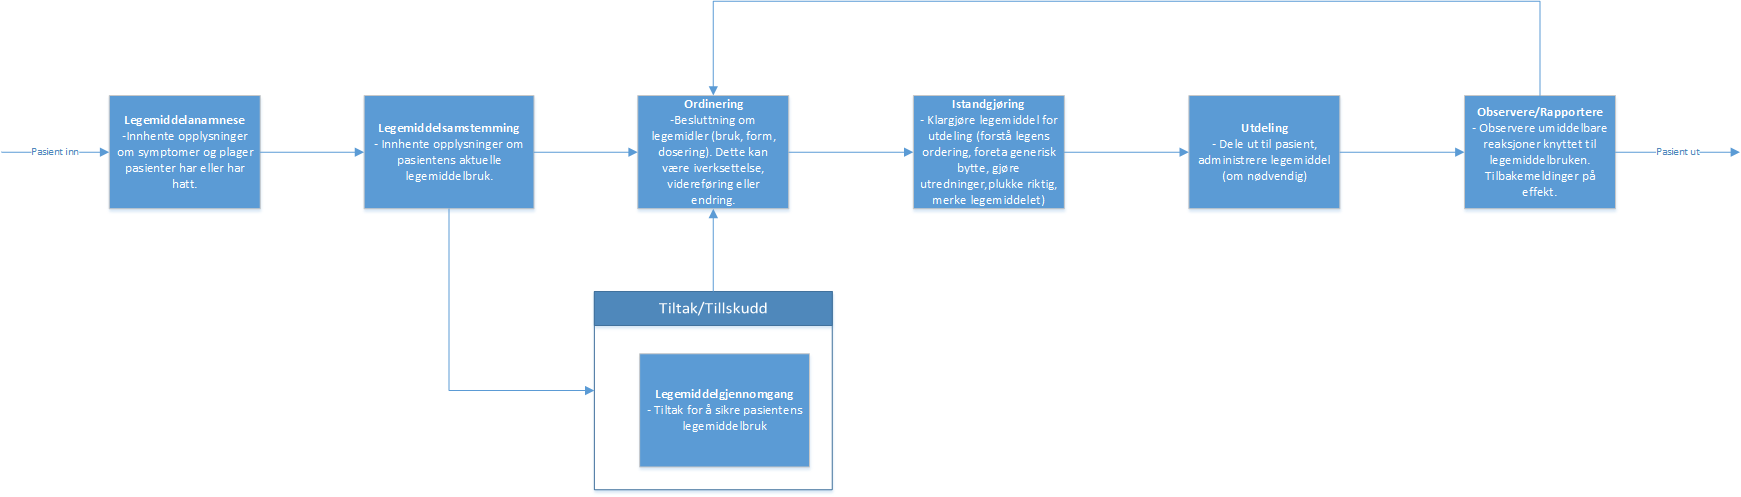
\includegraphics[width=18cm]{images/Legemiddelhandtering}
\label{fig:legemiddelhanderingsprosessen}
\caption{Legemiddelhåndtering i omsorgstjenesten}
\end{figure}
 
\subsection{Legemiddelanamnese} 
Riktig og fullstendig informasjon om pasientens pågående legemiddelbruk i sykehus er viktig for at all videre behandling skal bli så god som mulig. Anamnese er et medisinsutrykk for å hente informasjon som er basert på opplysninger som er gitt av pasienten selv. En anamnese skal inneholde opplysninger som symptomer og plager pasienten har eller har hatt. Anamnesen skal dokumenteres i pasientjournalen. Flere sykehus har et samarbeid i tverrfaglig team for å kunne sikre opptaket av anamnesen.

\subsection{Legemiddelsamstemming}
Da anamnesen skal ha informasjon om symptomer og plager til den enkelte pasient, skal en samstemming ta for seg legemidlene. En samstemming er en metode som helsepersonell, i samarbeid med pasient, utfører for å sikre korrekt overføring av pasientens aktuelle legemiddelbruk. Samstemmingen handler om at sykehuset, fastlegen, hjemmetjenesten, sykehjemmet, pårørenden og pasienten selv skal ha lik informasjon om pasientens faste legemidler. Hensikten er å sørge for at legemiddelinformasjon overføres korrekt ved overganger i pasientforløpet. Ved hver overgang sikres det at tiltak iverksettes for å sikre at det ikke er utilsiktede endringer som ikke indikeres. Dette kan være endringer i form av seponeringer, doseendringer eller ordinasjon. Hvis det er uoverensstemmelser i opplysningene skal dette redgjøres for og dokumenteres i pasientjournalen. 

\gls{lib} er en liste over legemidlene en pasient går på. Dette er en liste som blir laget under legemiddelsamstemming. Når denne listen blir laget skal tilgjengelige kilder brukes. Dette er kilder som EPJ, henvisning, epikrise, e-resept, multidose, PLO-melding eller pasientens egen liste. Her er det også viktig at det blir spurt om legemidler pasienten ikke tåler. \gls{lib} skal inneholde produktnavn, virkestoff, legemiddelform, styrke, dosering og bruksområde.\citep{Legemiddelverket_LMG}
 
\subsection{Ordinering}
Ordinering er prosessen der rekvirent bestemmer bruk av legemidler og at dette journalføres jf legemiddelhåndteringsforskriften §3 bokstav g. En ordinering kan være bestemmelse om å iverksette legemiddelbruk, videreføring, seponering eller endring av dosering. Rekvirent kan være lege, tannlege eller helsesøster. Ordinering skjer på bakgrunn av en faglig vurdering der rekvirent har sett behov for en endring av  pasientens legemiddelbehandling. I denne faglige vurderingen skal rekvirenten påse at bruken av legemidlene er forsvarlig for pasienten, som innebærer interaksjoner med andre legemidler, helsesituasjon, allergier og mer. 

Etter å bestemme bruk av legemidler må de bestilles. Rekvivering er prosessen ved muntlig, skriftlig eller elektronisk bestilling av legemidler jf legemiddelhåndteringsforskriften §3 bokstav f og forskrift om rekvirering og utlevering av legemidler fra apotek §1-3 bokstav e.  

\subsubsection{Legemiddelgjennomgang}
\ot{Forklar kort}
\ot{Tydeliggjør hvor dette skjer, konteksten.}
\ot{Ref forrige kap på en eller annen måte}
Tiltak for å sikre pasientens legemiddelbruk.

 

\subsection{Istandgjøring}
Istandgjøring er prosessen med å klargjøre legemiddel for utdeling jf legemiddelhåndteringsforskriften §3 bokstav i. Istandgjøring skal som hovedregel skje på grunnlag av orderingen gjort til enkeltpasient. Prosedyren er fastsatt av virksomhetsleder og utarbeidet av helsepersonell med rekvireringsrett for pasienten. Helsepersonellet som håndterer legemiddlene må forstå legens ordinering, eventuelt foreta generisk bytte\footnote{Generisk bytte er bytte til et likeverdig legemiddel som inneholder samme virkestoff i samme
mengde og i samme formulering.}, gjøre utredninger, sørge for å plukke riktig legemiddel og merke legemiddelet dersom legemiddelet ikke deles ut direkte. \citep{forskrift_legemiddelhandtering}

\subsection{Utdeling}
\ot{Hvem utdeler og hvor?}
Utdeling er prosessen hvor ferdig istandgjort legemiddel skal leveres ut til pasienten. Den som deler ut legemidlet må også kvalitetsikre utdeling. Dette vil si at den som leverer ut også skal observere inntaket, eventuelle umiddelbare eller senere reaksjoner av inntaket. Det må også vurderes og dokumenteres virkning og eventuell ikke-virkning av inntaket. Utdeling av legemidlene skal dokumenteres.

\subsection{Observere/Rapportere}
For å kunne ha en forsvarlig behandlig av pasienten må det oppstå regelmessige observasjoner av pasient. Med observasjon menes både observasjon av umiddelbare reaksjoner på gitt legemiddel og eventuelle reaksjoner som oppstår senere, men som kan knyttes til legemiddelbruken. Det må også komme tilbakemeldinger på manglenede effekt. Helsepersonell har også ansvar for å rapportere hvis det oppstår mistanke om kvalitetsvikt på legemidler eller utstyr. Observasjoner skal rapporteres til behandleransvarlig og dokumenteres i pasientjournalen.\citep{forskrift_legemiddelhandtering}


\section{Informasjonskilder og retningslinjer} \label{Informasjonskilder_og_retningslinjer}
I dette kapittelet skal vi se på ulike informasjonskilder og retningslinjer klinikere kan bruke når de foretar legemiddelgjennomganger i tillegg til legemiddelinformasjon.
\subsection{Pasientjournal} 
\subsection{Felleskatalogen}
Felleskatalogen er et oppslagsverk over farmasøytiske preparater til salgs i Norge. Her finnes en oversikt over preparater, vaksiner, naturlegemidler samt register over ATC-koder og substanser. I tillegg er det informasjon om spesielle tema som blant annet graviditet og forgiftning. All informasjon i felleskatalogen er enkelt tilgjengelig i et fritekstsøk. Felleskatalogen gis ut årlig og sendes ut gratis til alle helsepersonell-og institusjoner i Norge.
\subsection{RELIS}
Regionale legemiddelinformasjonssentre(RELIS) er en virksomhet som gjennom produktuavhengig legemiddelinformasjon har et mål om å bidra til rasjonell og korrekt legemiddelbruk. RELIS er i fire ulike regioner som holder kurs og seminarer for blant annet allmennleger og kliniske farmasøyter omkring riktig bruk av legemidler. RELIS har en felles nettside (www.relis.no) som publiserer nyheter og problemstillinger ved legemiddelbruk. Nettsiden har også en spørsmål-svar database for legemiddelrelaterte spørsmål. Her kan helsepersonell få hjelp, samtidig som at alle kan se tidligere spørsmål og svar. RELIS gir også muligheten for helsepersonell å melde inn bivirkninger via nettsiden. Avsender får en tilbakemelding etter en vurdering RELIS tar. Disse bivirkningene registreres også i en nasjonal bivirkningsdatabase.
\subsection{Renal Drug Database}
Renal Drug Database er en ressurs sammensatt av flere ulike kilder for å tilby helhetlig legemiddelinformasjon i forbindelse med pasienter som har nedsatt nyrefunksjon. Databasen tilbyr over 800 monografer med informasjon om klinisk bruk, interaksjoner, metabolisme og administrering. Denne ressursen er satt sammen av eksperter på området innenfor nedsatt nyrefunksjon og farmasi i Storbritannia. Med lisens har man full tilgang til kvalitetssikrede monografer, søkefunksjoner og verktøy som blant annet beregner Cockroft-Gault. Kliniske farmasøyter i Midt-Norge har lisens på Renal Drug Database.
\subsection{Epikrise}
Epikrise er en sammenfattet tekst som redegjør for årsak, utvikling og behandling av en pasient etter endt behandling. I de fleste tilfeller sendes epikriser etter endt sykehusopphold. Epikrisen sendes ut i henhold til §9 i pasientjournalforskriften. Pasienten har rett til å opplyse hvem epikrisen skal sendes til, men dersom ikke dette er spesifisert vil mottagere være henvisende helsepersonell samt pasientens fastlege. Motivasjonen bak epikrise er å sende relevant informasjon etter endt behandling til helsepersonell, slik at pasienten får nødvendig og forsvarlig oppfølging.

Det er ingen satte standarder i Norge for epikrisens struktur og innhold, men det finnes flere veiledninger omkring dette. Helsedirektoratet har utgitt en rapport som presenterer forslag til krav for innhold og struktur av den faglige delen av epikriser \citep{Den_gode_epikrise}. I rapporten er disse kravene kategorisert etter om de skal være obligatoriske eller anbefalte krav, i tillegg til når disse skal eller bør innføres. Hvorvidt disse kravene blir aktivt møtt er uvisst. I følge denne rapporten bør epikrisen, i tillegg til å ha praktisk informasjon om sykehus,utskrivende lege, tidspunkt og mer, inneholde informasjon om blant annet årsak til innleggelse,diagnose, kliniske prosedyrer, legemidler ved utskrivning, og vurdering. Siden denne informasjonen er ustrukturert, sendes epikrisen som fritekst.

\subsection{START, STOPP og NorGeP}
Screening Tool to Alert to Right Treatment(START) er en sjekkliste for forskrivning av legemidler til eldre. START er utviklet i Irland men er blitt oversatt til norske forhold. Listen brukes altså ved forskrivningsprosessen, og er delt opp i kapitler inkludert muskel- og skjelett, hormonsystemet, hjerte-og karsystemet, luftveien og mer. Under hvert kapittel er det forslag til legemidler eller type legemiddel som bør forskrives ved bestemte sykdommer.

Screening Tool of Older Persons’ Prescriptions er en sjekkliste for potensielt uhensiktsmessige forskrivninger til eldre. Denne er også utviklet i Irland og oversatt. Listen er strukturert på likt vis, og med mange av de samme inndelinger av kapitler. Her er det også listet legemidler under kapitler som går på ulike kroppsdeler/funksjoner, men her er dette legemidler som er uhensiktsmessig. Både i START og STOPP er det ingen detaljert forklaring på hvorfor typer legemidler bør forskrives eller seponeres.

The Norwegian General Practice(NorGeP) criteria er en liste over 36 kriterier over farmakologisk uhensiktsmessige forskrivninger til eldre pasienter i allmennpraksis. Her er legemidler gruppert etter område og beskrevet med generiske navn, i tillegg til en kort kommentar.

Felles for disse kriteriene er at de skal være til hjelp for å redusere suboptimale forskrivninger for eldre. En irsk studie har vist at bruken av START og STOPP gir resultater i praksis \citep{START_STOPP_GALLAGHER}. I hvor stor grad disse kriteriene er i bruk i Norge er uvisst. Samtidig kan kriteriene ha blitt en del av rutinen, slik at selve sjekklistene ikke blir brukt eksplisitt. START,STOPP og NorGeP er enkelt tilgjengelig for alle, så bruken av disse vil være vanskelig å måle. Flere fagpersonell vi har hatt kontakt med er kjent med disse kriteriene, og har samtidig uttrykt at disse ofte er satt opp på pauserom og lignende arealer, som en huskelapp.  
\subsection{E-resept}
\subsection{Legemidler i bruk}
Legemidler i bruk er meldinger som er en del av e-resept, og inneholder alle legemidler og andre relaterte varer som inngår i en samlet bruk for en pasient. Disse meldingene erstatter bruken av ordinasjonskort som før var i bruk i forbindelse med multidosering. Meldingen sendes fra multidoseringsansvarlig lege til apotek.
\subsection{Legemiddelhåndboka}
Norsk legemiddelhåndbok er et oppslagsverk om legemidler som behandling. Den er beregnet for allmennleger og institusjonslegen der vedkommende ikke er spesialist innenfor området. Derfor er det lagt vekt på å omtale tilstander som behandles hovedsakelig av disse legene, hvor legemidler har en viktig plass i behandlingen. I motsetning til FEST inneholder dette oppslagsverket detaljert informasjon om indikasjoner og bivirkninger av legemidler. Legemiddelhåndboken er delt inn i fire deler: 
\begin{itemize}
  \item Terapikapittler som tar for seg sykdommer i samsvar med WHOs sykdomsklassifikasjon
  \item Legemiddelkapittler som hører inn under terapikapittlene
  \item Generelle kapittler tar for seg grunnkunnskap innenfor farmakologi, og refusjonsreglene
  \item Registre 
\end{itemize}
Norsk legemiddelhåndbok finnes fritt tilgjengelig på nett i flere formater(\url{http://legemiddelhandboka.no/}), og som mobilapplikasjon.
\section{Kodeverk og standarder}
\subsection{ICD}
\gls{icd} er et internasjonalt kodeverk for klassifisering og registrering av sykdommer og andre beslektede helseproblemer. \gls{icd} er vedlikeholdt av \gls{who}, som er en del av FN. Alle sykdommer er klassifiserbare med bruk av \gls{icd}. Kodeverket er delt inn i ulike kapittler som igjen har sine egne kategorier. \gls{icd} blir oppdatert ved behov, og siste versjon er ICD-10 som ble publisert i 1994\citep{WHO_ICD}. Det er opp til hvert enkelt land å bestemme hvilken versjon av \gls{icd} man velger å benytte. I USA bruker de fortsatt ICD-7 fra 1962, men har samtidig oppdatert og tilpasset denne for å møte deres behov. Videre må \gls{icd} tilpasses og oversettes, da flere land har særegne klassifikasjoner.

I Norge brukes ICD-10 som er oversatt av KITH(Helsedirektoratet,avd standardisering). I Norge brukes dette kodeverket blant annet i spesialisthelsetjenesten, men også i andre områder som for eksempel i SSB for koding av dødsårsaker\citep{KITH_ICD}. Primærhelsetjensten bruker kodeverket ICPC.
\subsection{ICPC}
International Classification of Primary Care (ICPC) er et internasjonalt kodeverk for dokumentasjon av helseproblemer, diagnoser og symptomer som er brukt i primærhelsetjenesten. Her blir dette brukt ved konsultasjoner, henvisninger og forskriving av legemidler. Eksempelvis krever NAV at dette kodeverket brukes på alle attester der årsaken er sykdomsrelatert. ICPC ble første gang publisert 1987, og er utviklet av WONCA International Classification Committee(WICC). ICPC er nå i andre versjon og revideres fortløpende. I Norge brukes siste versjon, som er oversatt av KITH. 
\subsection{ATC}
Anatomisk, terapeutisk klassifikasjon(ATC) er et kodeverk som brukes for å inndele legemidler etter hvilket organ det virker på samt legemidlets virkemåte og egenskaper. Klassifiseringen brukes som basis for legemiddelstatistikk, i FEST(2.2.2) og i tilknytning til ICD-10(2.3.1). Systemet utvikles og vedlikeholdes av WHO.
\subsection{SNOMED-CT}
Systemised Nomenclature of Medicine-Clinical Terms (SNOMED-CT) er en terminologi som inneholder medisinske begrep, synonymer, koder, og definisjoner som er brukt i klinisk dokumentasjon. SNOMED-CT er ansett som den mest omfattende og flerspråklige terminologien for klinisk helsevitenskap\citep{Health_interoptability_HL7_SNOMED}. Hovedsakelig brukes denne for å gi bedre kommunikasjon og interoperabilitet på tvers av platformer. Norge er det eneste skandinaviske landet som ikke er medlem av IHTSDO.

\section{Personvern}\label{Personvern}
Digitale løsninger som bruker informasjon og personopplysninger gir store muligheter, men også visse problemstillinger knyttet til personvern. Behandling av sensitive opplysninger digitalt har den fordel med at det er lett tilgjengelig både internt i institusjonen i tillegg til pårørende og pasienten. Samtidig kan denne fordelen føre til at det blir enklere for uvedkommende å få tak i denne informasjonen. Dette kapittelet tar for seg lover og forskrifter som skal ivareta personvernet ved bruk av pasientspesifikk informasjon, og i vårt tilfelle i beslutningsstøttesystem.
\subsection{Personopplysningsloven og helseregisterloven}
Både personopplysningsloven og helseregisterloven har krav til informasjonssikkerhet. Det er Datatilsynet og Helsetilsynets ansvar for å se til at regelverket blir fulgt. Helseregisterlovens formål er "å legge til rette for innsamling og annen behandling av helseopplysninger (...) og gi bedre helse-og omsorgstjenester", jf. §1. Pasientspesifikk informasjon brukt i et beslutningsstøttesystem går i helseregisterloven under definisjonen av helseopplysninger jf. §2 punkt a. 

Personopplysningsloven er ment til å bidra til at personopplysninger skal behandles i tråd med grunnleggende personvernhensyn og informasjonssikkerhet. Helseregisterloven har regler for hvordan innsamling og behandling av helseopplysninger skal foregå. Reglene i helseregisterloven går i tråd med kravene som angår behandling av personopplysninger i personopplysningsloven. Begge lovene tar utgangspunkt i EUs personverndirektiv (95/46/EF).          

\subsection{Medisinsk utstyr}
Lov om medisinsk utstyr skal regulere "produksjon, markedsføring, omsetning og bruk av medisinsk utstyr", jf. §1. Dets formål er å "forhindre skadevirkninger, uhell og ulykker, samt sikre at medisinsk utstyr utprøves og anvendes på en faglig og etisk forsvarlig måte", jf. lovens §2. Loven gir klare detaljer om krav, merking og markedsføring, lagring og veiledning ved salg samt informasjon og bruk av medisinsk utstyr.

Lovens definisjon av medisinsk utstår er "(...)ethvert instrument, apparat, hjelpemiddel, materiale eller enhver annen gjenstand (...) ment å skulle brukes på mennesker", jf. §3 første ledd. Her er det en usikkerhet hvorvidt beslutningsstøtte med bruk av pasientspesifikk informasjon går under denne definisjonen. Lov om medisinsk utstyr §3 fjerde ledd, sier at i tvisttilfeller er det opp til Helse-og omsorgsdepartementet å avgjøre om et produkt faller innenfor kategorien av medisinsk utstyr.   

\subsection{Normen}
I 2002 tok Helsedirektoratet initiativ til å utvikle et sett med regler for trygg og sikker informasjonsutveksling. Dette initiativet kalles Normen, som utarbeider retningslinjer og krav for informasjonssikkerhet mellom ulike parter i helsesektoren. Normen er utviklet av representanter fra flere felt innenfor helse-, omsorgs- og sosialsektoren. Virksomheter kan forplikte seg ved avtale å følge Normen\citep{Normen}.

\section{Beslutningsstøtte}
\subsection{Klinisk beslutningsstøtte}
Klinisk beslutningsstøtte finnes i flere former som for eksemel retningslinjer som START og STOPP kriterier \citep{Bedre_legemiddelbehandling_av_eldre}. Evidensbasert medisin danner grunnlaget for slike retningslinjer ved bruk av randomiserte kliniske forsøk \citep{what_is_ebm}. Innen klinisk beslutningsstøtte har vi ikke kun slike "analoge" løsninger, men også digitale beslutningssystemer. Disse systemene kombinerer medisinsk kunnskapsdatabaser og algoritmer med spesifikk pasientdata og skal gi klinikere/brukere forslag til diagnose, prognose, monitorering eller behandling av individuelle pasienter \citep{european_commission}. 


\subsubsection{Evidensbasert medisin}
Innen forskning er en nødt til å ta hensyn til bevis. Medisin har i løpet av de siste 100 årene beveget seg gjennom faser hvor vi har gått fra at leger gjør seg opp egne meninger på hva som fungerer. Til enkle observasjoner innen medisin hvor pasienten av en eller annen grunn ikke ville motta behandling. Problemet med slike observasjoner er at de gruppene som mottar behandling og de som ikke gjør det ikke er tilfeldig valgte personer. Hvis en ser på litteraturen kan det se ut som sammenligningsgruppene se ut som en god miks fra populasjonen, men i virkeligheten kan det være andre grunner til at kontrollgruppen ikke fikk behandling. Hvis de i kontrollgruppen selv har valgt at de ikke vil ha behandling kan det være på grunn av for eksempel, en alternativ levestil. Dette kan resultere i at de på andre måter påvirker resultatet av studien på andre måter \citep[s.20-21]{cochrane1972}. Når en skal vurdere kriteriene for suksess kan en for eksempel vurdere subjektive kriterier som grad av effekt, men det enkleste er å ta hensyn om pasienten er død eller levende en viss periode etter behandling.

Det finnes bedre måter å utføre slike eksperimenter på, vi kan minimere slike mindre tilfeldige inndelinger av forsøksgruppen ved bruk av randomiserte, kontrollerte studier. I stedet for å se på "naturlige" inndelinger av forsøkspersonene skal gruppene bli valgt tilfeldig. Hverken pasient eller lege burde vite om pasienten er i kontrollgruppen eller ikke. Når legen heller ikke vet gruppen til pasienten blir dette kalt en "double blind" \citep[s.22-s23]{cochrane1972}. For å gjøre forsøkene så troverdige som mulig kontrolleres forsøkgruppen nøye slik at de passer inn under de kriteriene som legges til grunn. For eksempel kriterier som alder, diagnose og kjønn, dette for å prøve å luke ut ytre påvirkninger. Resultatet av slik forskning er veldig spesifikke resultater som passer til spissede forsøksgruppen.


\subsubsection{Kliniske retningslinjer}
Kliniske retningslinjer har sitt evidensgrunnlag fra evidensbasert medisin. Resultatet av slik forskning kan gi anbefalinger til behandling for veldig spesifikke tilfeller. Problemet med slike anbefalinger er at det nødvendigvis ikke passer veldig bra med populasjonen for øvrig.

Et stort problem, og økende  er problematikken rundt multimorbide. Multimorbide, pasienter med $\geq$2 kroniske lidelser, står for ca. 27\% av populasjonen og 66\% av de totale utgiften til helsevesenet i USA \citep{managing_MCC}.  Etterhvert som populasjonen øker, vil dette bli et enda større problem. I 1950 var det 8\% av populasjonen som var eldre enn 67 år, i dag er tallet 14\% og i 2050 er det estimert med 21\% eldre \citep{SSB_dette_er_norge}. Dette er en betydelig økning i eldre, og sammen med at over 50\% av populasjonen over 65 år er multimorbide, blir dette problem for fremtiden \citep[s.178]{OECD_health_reform}.



\subsubsection{Ekspertsystemer}


Ekspertsystemer er en gren innen kunstig intelligens(KI).\ot{nei, kunnskapsteknologi- som gir en beng i menneskelig resonnering eller kunnskap. Derimot korrekt og forutsigbar resonnering.} Dette er systemer som skal ha kunnskap om det domenet de er designet for og skal ha mulighet til å løse problemer innen dette domenet. Typiske bruksområdet ligger innenfor datatolkning(sonarsignaler) og diagnostisering av feil(feil i utstyr eller sykdom i mennesker), samt analyse av kompliserte strukturer og planlegging av avgjørelser for en robot \citep[s.2]{intro_expertsystems}.

Det som skiller et ekspertsystem fra et vanlig dataprogram er:
\begin{itemize}
\item Simulere menneskelig resonnement innen problemdomenet i stedet for å simulere domenet i sin helhet.
\item Skal utføre resonnement over en representasjon av menneskelig kunnskap. Kunnskapen til systemet er ofte skrevet i et språk designet for kunnskaprepresentasjon. Kunnskapen er moddelert i en kunnskapsbase og systemet resonnerer med en "inference engine" samt annen logikk.
\end{itemize}\citep[s.3]{intro_expertsystems} 


Ekspertsystemer er systemer som løser problemer med realistisk kompleksitet som ofte krever menneskelig tolkning. De skal løse virkelige problemer innen forskning eller av kommersiell interesse. Systemet må ha en høy ytelse, både i hastighet og robusthet. Et slikt system opererer som en ekspert og brukeren av systemet forventer svar innen rimelig tid. Systemet skal også kunne gi en forklaring for sitt resonnement og løsning, slik at brukeren kan se grunnlaget for beslutningen\citep[s.3]{intro_expertsystems}.

Kunnskapsbasen fylles med ved et samarbeid mellom en informatiker og en ekspert innen domenet systemet skal lages for, for eksempel en lege. Innhenting blir ofte en flaskehals under utvikling av slike systemer og det er estimert at et slikt team kan lage mellom 2 og 5 fakta om dagen. Problemer innebærer forskjellig fagspråk, en ekspert har ofte problemer med å formidle sin kunnskap i et dagligdags språk. Eksperter trenger også å vite mer enn bare de enkle fakta og prinsipper om et domene for å løse problemer. For eksempel, de vet hvilken informasjon som er relevant for det problemet de skal løse. De er også flinkere på å dele vanskelige problemer ned i mindre, enklere problemer som kan løses individuelt. Å modellere slik kunnskap, som ofte er basert på personlige erfaringer er mye vanskeligere og kan være en svakhet til et slikt system\citep[s.3-4]{intro_expertsystems}.

\subsection{Juridiske problemer knyttet til beslutningsstøtte}
Beslutningsstøtte skal hjelpe en bruker med å fatte en korrekt beslutning, men hvilken part er skyldig hvis en beslutning fattet ved hjelp av beslutningsstøtte, får kritiske konsekvenser?  Dette er en problemstilling som berører både brukeren, beslutningsstøttesystemet i tillegg til eventuelle forfattere av innholdet brukt i systemet. Er for eksempel en juridisk ansvarsfraskrivelse tilstrekkelig for å unngå et søksmål? Hvis informasjonen og reglene brukt i beslutningsstøttesystemet er åpne og fritt tilgjengelige data, kan forfatterne bak innholdet da være skyldige?

Her er det dessverre ikke noen definitive svar. En artikkel fra 2007 som så på muligheter og problemstillinger knyttet til bruk av SOA(Service-Oriented Architecture) i kliniske informasjonssystemer,  
sier at tjenester er ikke lisensierte klinikere, så juridisk vil institusjonen eller utøveren være ansvarlig for å se bort i fra råd gitt av systemet som kan være skadelige\citep{SOA_DSS}. Videre argumenterer forfatterne at dette utgangspunktet kan minske brukernes tillit til bruken av disse tjenestene. Her må vi si oss uenige, da dette også kan sies om anvendelsen av retningslinjer, kildereferanser og annen litteratur innenfor medisin. Disse er mye brukt, selv om forfatterne ikke tar ansvar for eventuelle konsekvenser.

\section{Teknologi\ot{Veldig langt kapittel(mangler mye subsections), kan vi flytte ut til eget kapittel? Veldig sentralt for oss dette}}
I dette kapitellet ser vi på teknologi som eksisterer og som i tillegg kan være til nytte i å svare på forskningspørsmålet jf. delkapittel \ref{innled:forskningsporsmal}. 
\subsection{Ontologi}
\label{bakg:ontologi}
I kunnskapsteknologisk litteratur finnes det flere definisjoner om hva en ontologi er, og mange av disse er i strid med hverandre. For formålet med vårt studie er en ontologi et konsept som presist formulerer beskrivelser i et domenet. I en ontologi inneholder det klasser (også kalt konsepter), egenskaper som beskriver funksjoner og attributter for hvert konsept og restriksjoner for egenskapene. En ontologi sammen med et sett av instanser utgjør en kunnskapsbase. Et instans er et objekt av en klasse.\\
Klasser er sentralt i ontologier. Klasser beskriver konsepter i et domene, for eksempel kan vi ta for oss klassekonseptet mennesket. Et hver spesifikk menneske vil da være et instans av klassen Mennesket. Håvard Moås ville vært et naturlig instans av klassen Mennesket. Klasser kan også ha subklasser, hvor en artist kunne vært en subklasse av klassen person. \\
Egenskaper (properties) beskriver egenskaper til en klasse og ett instans. Håvard Moås har egenskaper ved å være et menneske, mennesker har et kjønn og finnes i forskjellige raser. Her har vi da to egenskaper som kobler mennesket sammen med et kjønn og rase. (Visualisert i figur 4.1). Under hver klasse er det instanser av hver klasse. For å ha resonneringstøtte kan inverse og symmetriske egenskaper være lurt, vi vil komme nærmere tilbake til dette i kap 4.2.4. % TODO: se over at kapittel stemmer


\begin{figure}[H]
\centering
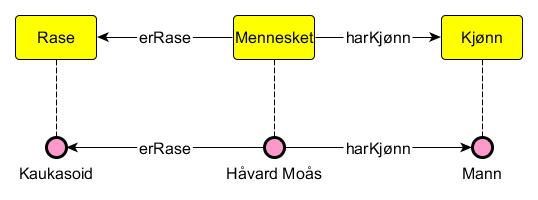
\includegraphics[width=10cm]{images/ontologi_eksempel.jpg}
\caption{Eksempel på klasser og egenskaper i en ontologi }
\end{figure}

I praksis inkluderer utvikling av en ontologi å:
\begin{itemize}
\item Definere klasser i ontologien.
\item Arrangere klassene i et taksonomisk (subklasser-subegenskaper) hierarki.
\item Definere egenskaper og beskriv lovlige verdier for disse egenskapene.
\item Fylle inn verdier for disse egenskapene og klassene i form av instanser.
\end{itemize} \citep{ontology_101}
\subsection{Semantisk teknologi}
\subsubsection{Visjon}
Det er ingen fast definisjon på semantisk web, men heller en visjon om at maskiner skal kunne forstå meningen bak innholdet på internett. Begrepet er skapt av W3C, som også  utvikler, vedlikeholder og tilrettelegger teknologier og metoder som brukes for å realisere denne visjonen. Ifølge skaperne av begrepet “gir semantisk web et felles rammeverk som tillater data til å bli delt og gjenbrukt på tvers av applikasjoner, bedrifter og samfunnets grenser”\citep{W3C_semantic_web}.  

For å realisere denne visjonen må det tas designvalg for semantisk web. Disse kan bli summert slik: 
\begin{enumerate}
    \item lage strukturerte, semi-strukturerte data tilgjengelig i standardisert format på web;
    \item ikke bare lage datasett, men også individuelle dataelementer og deres relasjoner 	tilgjengelig på web;
    \item Beskrive den tiltenkte semantikken i en formalisme, slik at den tiltenkte semantikken kan prossesseres av maskiner\citep{webprimer}.
\end{enumerate}
Det er mange muligheter som oppstår ved å gjøre webens innhold mer tilgjengelig for maskiner. Maskiners rolle i den tradisjonelle weben er for det meste å overføre informasjon fra tjener til klient og indeksere søkeord. Ved hjelp av semantisk web kan maskiner gjøre mye av det intelligente arbeidet, som for eksempel aggregering og kombinering av data. Søking trenger ikke å være begrenset til nøkkelord; Ved hjelp av semantisk forståelse av selve søket kan dette inkludere synonymer, hensikt, kontekst av søk med mer. Nettsider kan bli mer personlig tilpasset hvis spesifikke agenter kan forstå innholdet av nettsiden og samtidig tilpasse dette til brukerprofiler.    
\subsubsection{Semantiske teknologier}
De designvalg som er nevnt tidligere må også være beskrevet i bestemte teknologier. Disse teknologiene er også basisen for semantisk web, som beskrevet av W3C:
\begin{enumerate}
\item Grafer som datamodell for objekter og deres relasjoner, der et objekt er en node i grafen og en kant representerer relasjoner mellom objekter. For dette brukes RDF(Resource Description Framework).
\item Web-identifikatorer(URI) for å identifisere objekter og relasjoner. Disse er også beskrevet i RDF.
\item Ontologier som datamodell for å representere den tiltenkte semantikken av data. Her brukes OWL(The Web Ontology Language) og RDF Schema som formalismer, som igjen bruker URI for å representerer typer og egenskaper.
\end{enumerate}

Videre må det også være mulig å hente og manipulere data fra disse strukturene gjennom spørringer. SPARQL er et spørrespråk utviklet av W3C som også har gjort dette til en standard.  

Semantisk web kan tenkes å være utviklet lagvis, der hvert lag er bygget oppå et annet lag. Grunnen til denne lagdelingen er todelt. En ting er at det er enklere å få konsensus i miljøet for små steg som tas enn større endringer foreslås. Fra et annet perspektiv er denne lagdelingen viktig med tanke på standardisering. I utviklingen av semantisk web er det stor konsensus på at følgende to prinsipper burde bli fulgt når et lag bygges oppå et annet:
\begin{itemize}
\item En programvarekomponent som er oppmerksom på et lag burde være i stand til å forstå og bruke informasjon lagd på lavere nivå. Hvert lag burde altså være nedover kompatibel.
\item Det skal være mulig for en programvarekomponent å delvis ta utnytte av informasjon fra høyere lag. Dette er mulig hvis en kan ignorere komponentene som overgår nettopp laget denne programvarekomponenten er brukt til. Eksempel kan være at en komponent oppmerksom på RDF og RDFS kan delvis tolke informasjon skrevet i OWL. 
\end{itemize}

Denne lagdelte arkitekturen har vært en gjeldende visjon i utviklingen av semantisk web. Dessverre har ikke utviklingen gått helt denne veien, og noen kompromisser har vært nødvendig å ta på bekostning av prinsippet om nedover kompatibilitet. Mer om dette i kap 4.1.3.  % TODO: se over at kapittel stemmer

Figur 4.1 viser den lagdelte arkitekturen for semantisk web. Unicode og URI-laget sørger for at vi bruker internasjonale tegnsett og muliggjør identifisering av objekter. XML-laget med NameSpace og skjemadefinisjon gjør det mulig å integrere definisjoner fra semantisk web med XML-baserte standarder. Med RDF og rdfschema kan man opprette påstander om objekter med URI, samt definere egne modeller. Ontologier er en form for kunnskapspresentasjon. Dette laget sørger for muligheten til å representere mere komplekse relasjoner mellom objekter. Logic-laget kan tenkes å være en utvidelse av Ontologi-laget; Et resonneringssystem for økt funksjonalitet og muligheten til å manipulere applikasjonsspesifikk deklarativ kunnskap. Trust-laget sørger for utførelsen av reglene definert av ressonneringssystemet, og sammen med Proof-laget utgjør mekanismen for applikasjoner å stole på bevis. De to øverste lagene i modellen skal sikre kvaliteten på informasjonen.

\begin{figure}[H]
\centering
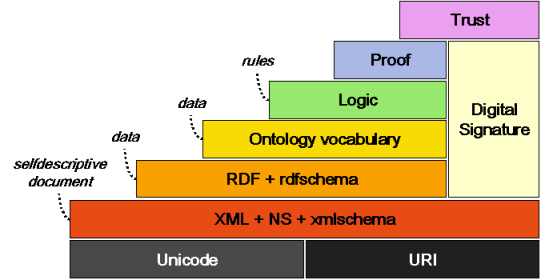
\includegraphics[width=90mm]{images/swlevels.png}
\caption{Semantisk web lag }
%\label{overflow}
\end{figure}

\subsubsection{Open world assumption}
Open world assumption er et prinsipp brukt i forbindelse med kunnskapsrepresentasjon, som sier at et utsagn kan være riktig uavhengig av om man \textit{vet} at utsagnet er riktig eller ikke. Dette er da det motsatte av det som kalles "Closed-world assumption", som sier at ethvert utsagn som er riktig faktisk er riktig. Semantisk web kan ikke ha et "closed-world assumption", siden en kan aldri vite om flere ressurser er beskrevet på flere ulike måter ute på internett. I tillegg kan man ikke vite om disse er beskrevet med bruk av samme type skjema eller ha like egenskaper. Et eksempel på dette kan være at man har flere universiteter, og noen av disse er mer beskrevet enn andre, og kanskje bruker et annet vokabular i tillegg. Instansene kan også beskrive samme universitet! 

\subsubsection{Resource Description Framework}
RDF er et formelt språk brukt for å beskrive informasjon. I motsetning til HTML og XML, der målet er å vise dokumenter riktig, er målet til RDF å bevare meningen bak dokumentet på tvers av applikasjoner på web. På denne måten kan denne informasjonen prosesseres videre og kombineres på ulike måter. RDF er ansett som det grunnleggende representasjonsformatet ved utviklingen av Semantic Web.

Kort sagt beskriver RDF generelle relasjoner mellom ressurser. RDF er basert på en graf-orientert dataskjema, der et dokument beskriver en rettet graf. Med andre ord har man et sett med noder som er lenket med direkte kanter. Både nodene og kantene er merket med unike ID'er. En node kan unntaksvis være blank, altså at den representerer objekter som ikke har egne navn. En ID kan være i form av et navn eller en Uniform Resource Identifier. Sistnevnte er en generalisering av URL(Uniform Resource Locator), som er en streng brukt til å finne websider i en nettleser. Med andre ord så er URI en identifiserbar og navngitt ressurs ved hjelp av lokaliseringsinformasjon.

Nodene og kantene i RDF-dokumenter blir omtalt som tripler. Dette er en setning med strukturen subjekt-predikat-objekt. En slik trippel danner en rettet graf, der kantene er forbindelsen mellom to ressurser. Med andre ord representerer kantene i en RDF-trippel forholdet mellom to ressurser. På denne måten kan RDF gi muligheten til å dele strukturert informasjon på tvers av applikasjoner.

\begin{figure}[H]
\centering
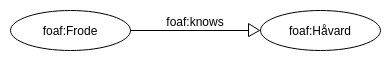
\includegraphics[width=90mm]{images/rdf_triple.png}
\caption{Eksempel på RDF trippel}
% \label{overflow}
\end{figure}
\subsubsection{Resource Description Framework Schema}
RDFS er et sett med klasser og tilhørende egenskaper bygd på RDF; Et vokabular for RDF som gir ytterligere ekspressivitet. Disse klassene og egenskapene gjør at RDFS kan sees på som et språk for kunnskapsrepresentasjon eller et ontologispråk, som kan i stor grad beskriver semantisk gjensidige avhengigheter innenfor et domene. Selv om RDFS kan sees på som et ontologispråk, har den sine begrensninger. Derfor er det mange som kaller RDFS et representasjonsspråk for lettvekts-ontologier. Mer sofistikerte applikasjoner krever et mer ekspressivt representasjonsspråk. Andre vokabularer av RDF, for eksempel OWL, bruker RDFS i bunn. 

Klasser og egenskaper i RDFS kan på flere måter sees likt på som i objektorienterte programmeringsspråk. En kan for eksempel tilegne en instans av en klasse egenskaper til en annen klasse. En hund har den egenskap at den er et dyr. Likevel er det fundamentale forskjeller. Alt i RDFS er klasser, også egenskaper. Egenskaper i RDFS er igjen instanser av klassen rdf:property, som igjen er en instans av klassen rdf:class. Klassehierarkier i objektorientert programmering representerer strukturer som kan sees på som mer statisk. Ved ontologispråk som RDFS representerer disse hierarkiene informasjon ute på internett som kan være i konstant utvikling. I tillegg til dette er ontologier langt mer fleksible, i og med at denne informasjonen kommer fra heterogene kilder.

RDFS gir mulighet til å beskrive hierarkier av klasser og egenskaper, sette restriksjoner på ressurser, definere ressurser som datatype,literal og ressurs samt definere lister.
\subsubsection{Web Ontology Language}
Web Ontology Language(OWL) er et språk for kunnskapsrepresentasjon i likhet med RDFS; et vokabular for RDF. Som allerede nevnt er RDFS noe begrenset, og tilbyr mer eller mindre kun klasse- og egenskaphierarkier, samt sette flere typer restriksjoner på disse. Ved flere tilfeller så trenger man et mer ekspressivt språk for kunnskapsrepresentasjon. Et eksempel kan være at alle personer har en bursdagsdato, og at ingen person er både mann og kvinne. OWL tilbyr nettopp slik funksjonalitet. 

OWL er bygd på en familie av logikkspråk, eller rettere sagt Description Logics som er laget spesielt for å representere terminologisk kunnskap. Description Logic er en samling språk for kunnskapsrepresentasjon, som inkluderer blant annet OWL. Disse språkene gir mulighet for å beskrive blant annet klassemedlemskap, klassifisering, ekvivalens og likhet, disjunkthet og ulikhet, kardinalitet, sette lokalt "scope". I tillegg til dette tilbyr OWL automatisert resonnementstøtte. Dette sikrer at et ontologi er logisk korrekt, og innebærer sjekk for konsistens og utilsiktet relasjoner mellom klasser og instanser. 

Det er ikke mulig å ha automatisk resonnementstøtte i kombinasjon med ekspressiviteten beskrevet ovenfor. Derfor er OWL delt opp i to ulike subspråk for å fylle de ulike kriteriene.
\subsubsection{OWL Full}
OWL Full er språket i all sin helhet. Det tillater all mulig kombinering av OWL-primitiver med RDF og RDFS. OWL Full har en RDF-basert semantikk som gjør at den er nedover kompatibel. Det vil si at ethvert korrekt RDF dokument er også et OWL Full dokument, og enhver slutning i RDFS er også en korrekt slutning i OWL Full. På en annen side gjør dette, i tillegg til vilkårlig bruk av primitiver, at automatisk resonnementstøtte i OWL Full ikke er mulig. Språket er med andre ord så fleksibelt at det ikke er mulig å trekke noen slutninger om korrekthet.
\subsubsection{OWL DL}
OWL DL er et subspråk av OWL som er "mappet" mot Description Logic. På dette viset er det mulig med god resonnementstøtte. Det eksisterer flere tolkere til dette, inkludert Pellet, FaCT,RACER og HermiT. En bakside ved dette er at det begrenser ekspressiviteten som OWL Full har. 

Den største ulempen ved OWL DL er at den ikke er fullt kompatibel med RDF. Dermed bryter dette med den lagdelte arkitekturen og prinsippet med at hvert lag skal være nedover kompatibelt som beskrevet i kap 4.1. Det er kun ved OWL Full at dette prinsippet blir fulgt, dog på bekostning av muligheten for resonneringsstøtte.    

\subsubsection{SPARQL Protocol and RDF Query Language}
SPARQL er et spørrespråk for å hente og manipulere kunnskap uttrykt i RDF. Spørrespråket er utviklet primært for RDF og har flere likheter med spørrespråk for tradisjonelle databaser. Det finnes flere spørrespråk for RDF, inkludert DQL og N3QL. SPARQL er spørrespråket W3C anbefaler og er gjort til en standard. Fleste populære programmeringsspråk har API'er tilgjengelig for å prosessere og lage SPARQL-spørringer.

For å kunne utføre en spørring må man ha en triple store tilgjengelig, som kan sees på som en RDF-database. I dokumentasjonen for SPARQL refereres disse som "graph store". Hele denne databasen er med andre ord et sett med tripler som beskrevet i kapittel 4.1.2. SPARQL har mekanismer for hente, legge inn og fjerne tripler i en triple store. Man har fire ulike type spørringer i SPARQL, men alle følger et bestemt mønster. Grunnlaget er at en SPARQL-spørring konstrueres som et grafmønster, der databasen finner tripler som har et likt mønster. I SPARQL kan man erstatte subjekt, predikat og objekt med variabel. Hvis en ønsker å hente ut alle tripler fra databasen, er det bare å sende inn et grafmønster med kun variabler. Resultatene av en spørring kan gjøres tilgjengelig på flere maskinlesbare formater, inkludert XML og JSON.

\begin{figure}[H]
\centering
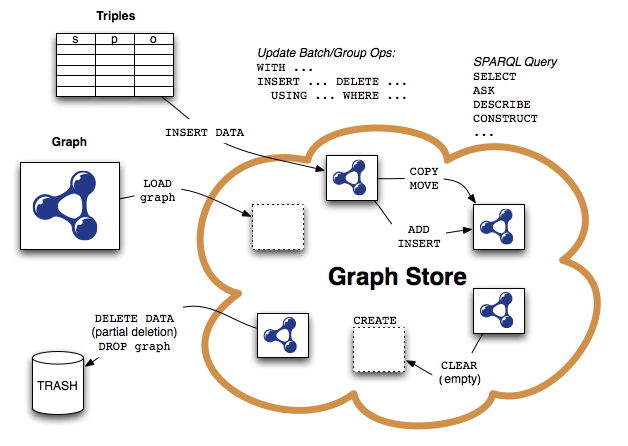
\includegraphics[width=140mm]{images/sparql_endpoint.png}
\caption{SPARQL endpoint }
%\label{overflow}
\end{figure}
%TODO: REFERER DETTE BILDET TIL :https://www.dajobe.org/blog/

\subsubsection{Semantiske teknologier i helse-og biovitenskap}
Mange har sett nytten i å bruke semantiske teknologier innenfor helse-og biovitenskap. Dette feltet har store problemer med heterogene data spredt over ulike domener. Samtidig vokser datamengden i dette feltet. Forskere og andre må kunne foreta spørringer som går på tvers av disse for å kunne ta kritiske avgjørelser. Bruk av semantiske teknologier kan redusere kostnadene ved en slik integrasjon av datakilder. Hvis dette skal være mulig må data om legemidler, sykdommer, pasienter, proteiner, celler og reaksjonsveier være tett integrerte. Samtidig må et felles vokabular må være på plass, med definisjoner, koder, synonymer og begreper. For at sektoren skal kunne se hvilke fordeler bruk av semantisk web innebærer, må en aktør aktivt fremme interesse og muligheter dette fører med seg. W3C opprettet Semantic Web for Health Care and Life Sciences Interest Group for å utvikle, støtte samt være en pådriver for bruken av semantiske teknologier i helse-og biovitenskap\citep{W3C_HCLSIG}. Noe av arbeidet de har gjort er å publisere genomiske og legemiddelrelaterte datasett som RDF-tripler. 

\subsubsection{SNOMED-CT}
For at man skal kunne integrere heterogene datakilder, må et felles vokabular på plass. Systemised Nomenclature of Medicine-Clinical Terms (SNOMED-CT) er en terminologi som inneholder medisinske begrep, synonymer, koder, og definisjoner som er brukt i klinisk dokumentasjon. SNOMED-CT er ansett som den mest omfattende og flerspråklige terminologien for klinisk helsevitenskap\citep{Health_interoptability_HL7_SNOMED}. Hovedsakelig brukes denne for å gi bedre kommunikasjon og interoperabilitet på tvers av platformer. SNOMED-CT er ikke direkte tilgjengelig i OWL-format, men er utgitt som en egen filstruktur kalt Release Format 2. Andre leverandører som Snow Owl IDE\citep{Snow_owl} og skript i ulike programmeringsspråk støtter eksportering til OWL. 

Terminologien eies og drives av International Health Terminology Standards Development Organisation, som ble startet i 2009 av 9 medlemsland. I dag har organisasjonen over 20 medlemsland over hele verden, samtidig som de har gitt ut lisenser for mer enn 5000 individer og organisasjoner\citep{IHTSDO_members}. For å kunne bruke SNOMED-CT eller utvikle programvare som bruker SNOMED-CT må en ha lisens. Norge er det eneste skandinaviske landet som ikke er medlem av IHTSDO. En rapport fra KITH(nå underlagt Helsedirektoratet) fra 2009 konkluderer at SNOMED-CT bør prøves i bruk innenfor et område i helsesektoren der det er et sterkt behov for en standardisert terminologi \citep{KITH_SNOMED-CT}. Samtidig nevnes det at behovene for en slik terminologi vil bli mer åpenbar med tiden, da innholdet i elektroniske informasjonssystemer blir mer strukturert i helsesektoren. Selv om Norge ikke er et medlemsland, er det flere og flere aktører som åpner opp for bruken av denne terminologien. Dips Arena er Dips sitt tredjegenerasjons pasientjournal som kommer til å bruke OpenEHR, som er en åpen kodeplattform for elektronisk pasientjournal. Dette, sammen med arketyper, skal danne basisen for en mer strukturert pasientjournal\citep{Dips_OpenEHR}. OpenEHR har støtte for flere fagterminologier, inkludert SNOMED-CT. I tillegg er det flere arketyper som forutsetter bruk av slike terminologier. Dips Arena er forventet å være ute i produksjon i løpet av 2016. Et nytt norsk insentiv har utviklet en plattform(http://www.magicapp.org/) for å utvikle og oppdatere pålitelige retningslinjer som beslutningsstøtte i elektroniske pasientjournaler(Her menes EMR, hva er det på norsk?). Rammeverket bruker nettopp SNOMED-CT, og andre kjente ontologier i norsk helsevesen som ICD-10, for å komme med pasient-spesifikke anbefalninger\citep{MAGIC_HelsIT}. Selv om flere åpner opp for bruken av SNOMED-CT i Norge, har det aldri vært i klinisk bruk her.

Selv om tanken bak et felles begrepsapparat på tvers av landegrenser virker lovende, har flere institusjoner og land vært avventende til SNOMED-CT. Flere mener at SNOMED-CT i dagens tilstand er utdatert og i overkant komplisert. Samtidig er det også funnet flere kritiske feil i terminologien. En studie \citep{Rector-SNOMED-CT-1} foretok bruk av terminologien i to praktiske prosjekter, for å finne mulige problemstillinger knyttet opp mot denne terminologien og hvordan eventuelt adressere disse. De fant systematiske feil knyttet opp mot sentrale konsepter innen medisin, inkludert hypertensjon og diabetes. Studien konkluderte med at de som brukte SNOMED-CT på denne tiden(2011) burde være varsomme, da feil i hierarkiene eller et forsøk på å rette disse opp ville sannsynligvis føre til meningsløs bruk av terminologien. En nyere studie \citep{Rector-SNOMED-CT-2} studerte SNOMED-CT som et eksempel på å bruke et metodeverk for å finne feil i biomedisinske ontologier, fant ytterligere feil i terminologien som ikke er tidligere oppdaget.

\subsubsection{ICD\ot{vurder å fjern dette? vi nevner det i et tidligere kapittel}}
En annen internasjonal standard for felles terminologi i helseverden er \gls{icd}. Kodeverket er et redskap for klassifisering og registrering av sykdommer og andre beslektede helseproblemer. \gls{icd} er vedlikeholdt av \gls{who}, som igjen er en del av FN.  
\subsection{Informasjonskilder}
\subsubsection{DrOn}
\gls{dron} er en modulær ontologi for legemiddel-produkter utviklet med semantiske teknologier. Den innehar informasjon om ingredienser og biologisk aktivitet med utgangspunkt i legemidler som selges i USA \citep{dron_2013}. Ontologien bruker RxNorm som dets eksterne hovedkilde, som er en medisinsk terminologi som inneholder alle legemidler til salgs i USA. Disse legemidlene er kartlagt opp mot ChEBI-klasser. \gls{chebi} er en database og ontologi som inneholder molekylære entiteter. Resultat av dette er at en kan resonnere mellom legemidler med tilhørende ingredienser og biologiske aktivitet. 

For å lage denne ontologien minet de data fra utgivelser av RxNorm. Dette ble gjort ved å laste ned råfilene, omforme dataene for å deretter importere dette i en relasjonsdatabase ved hjelp av et skript som er tilgjengelig. Så ble RxNorm-entiteter kartlagt opp mot ChEBI-klasser ved hjelp av en konsollapplikasjon som sammenlignet etiketter av ingredienser i RxNorm med klasseannoteringer i \gls{chebi}. Deretter ble den normaliserte databasen oversatt til en OWL-artefakt. 

\gls{dron} er modulært, slik at klasser fra hver kilde er serialisert i separate moduler som igjen er konsumert(del av..) av klasser som er manuelt utarbeidet på et høyere nivå i en modul med termer som «klinisk rolle», «tablett», «kapsel» med mer. På denne måten kan en enkelt bruke deler av ontologien i tillegg til at videreutvikling vil være enklere. 

Denne ontologien inneholder mye informasjon om legemidler, og kan spille en viktig rolle i utviklingen av vårt system. Framgangsmåten deres kan være nyttig for oss, selv om vi velger å ikke ta i bruk \gls{dron}. Hvis vi går for å bruke \gls{dron} på en eller annen måte, er det visse aspekter med ontologien vi må ta stilling til. Den største problemstillingen vil nok være å bruke denne ontologien i norsk sammenheng. Er det mulig å koble amerikanske legemidler opp mot legemidler til salgs i Norge? 
\subsubsection{FEST} \label{FEST}
Forskrivning-og ekspedisjonsstøtte (FEST) er en database utviklet av Statens Legemiddelverk som inneholder oppdatert informasjon om alle legemidler en kan få på resept i Norge. I FEST er det for hvert legemiddel oppgitt informasjon om blant annet pakningsvedlegg, dosering, inntaksmåte, virkestoff og interaksjoner med andre legemidler. FEST brukes som datagrunnlag i systemer for blant annet e-resept, felleskatalogen, interaksjoner.no, allmennlegesystem, kommunal pleie og flere sykehus.

Databasen er i dag tilgjengelig i XML-format. Statens Legemiddelverk jobber nå for å gå bort i fra XML-formatet, og levere FEST som åpne, lenkede data. Dette kaller de femstjerners FEST, som referer til Tim Berners Lee 5-stjerners skala for publisering \citep{Femstjerner_FEST}. Dette innebærer å bruke semantiske teknologier for å gjøre data tilgjengelig på web, samt lage lenker som gir muligheten til å utforske data. En testutgave av femstjerners FEST er tilgjengelig og inneholder kun "varsel fra SLV". Varsel fra SLV(Statens Legemiddelverk) er notis sendt til lege med sikkerhetsinformasjon knyttet til legemidler. Dette kan for eksempel være et varsel om en uheldig bivirkning som ikke er tidligere kjent. 
\subsection{MedExt - Samstemmingsmodul}
MedExt er navnet på samstemmingsverktøyet utviklet av Vivit ved NTNU. Dette verktøyet ble utviklet ved oppdrag fra Norsk forening for allmennmedisin, og brukes i dag av allmennleger i store deler av landet. Medext er en programvarekomponent som er integrert i deres EPJ-system. Her fungerer Medext som prosesstøtte ved samstemmingen av legemiddellister. Det vil si at komponenten vil gjøre det enklere å foreta en samstemming ved å strukturere informasjon fra fritekst og sette denne listen opp mot \gls{lib}. Denne friteksten er som oftest en epikrise eller PLO(Pleie og Omsorg)-melding.



\section{Metode}
\ot{Fjern navnet på dette kapitellet? Gir ikke helt mening mtp plan og valg}
\ot{Vurdere dette kapitellet, kanskje ha mer bakgrunnsinformasjon om forskningsmetode}
\subsection{Forsøk}
Forsøk er en måte å undersøke sammenhenger mellom årsak og virkning, ved å bevise eller motbevise en sammenheng mellom en faktor og et utfall \citep[s.126-127]{Researching_is}. I vårt tilfelle undersøker et forsøk hvordan vårt system vil påvirke relasjonen mellom utførelsen av legemiddelgjennomgang og aspektene tidsbruk, riktighet og kunnskapsoverføring. Et forsøk skal være konstruert for å besvare en hypotese, altså en påstand om at en faktor er en årsak til en virkning. Hypotesene vil bli utarbeidet senere i forskningsprosessen, men vi vil anta at disse har en lignende ordlyd som forskningsspørsmålene ovenfor.    

Forsøk kan bli utført i ulike omgivelser. Man skiller forsøk typisk mellom utførelse i lab og utførelse i naturlige omgivelser, også kalt feltforsøk. Førstnevnte lar en isolere variablene, slik at disse kan bli studert og kontrollert nøye. Samtidig er slike forsøk satt i et kunstig miljø, slik at variablene vi selv fokuserer på kan endre seg grunnet en annen ytre variabel som ikke eksisterer eller er tatt hensyn til. Et feltforsøk vil være nærmere virkeligheten, men på en annen side blir det langt vanskeligere å manipulere variablene vi er interesserte i grunnet ytre faktorer. Med tanke på ressursene og tidsbruken vi har, har vi valgt å gå for et labforsøk. Det vil både være enklere og mindre tidkrevende å gjennomføre. Feltforsøk vil være problematisk med tanke på rekruttering og formelle godkjennelser fra flere hold.  

Et spesifikt forsøksdesign bør velges ut i fra om denne utførelsen sikrer at en endring i virkning skyldes kun årsaken vi definerer \citep[s.134-135]{Researching_is}. I vårt tilfelle vil det for eksempel si at hvis vi har en hypotese om at legemiddelgjennomgang vil være mer effektivt med vårt system i bruk, bør vi velge et forsøksdesign som sikrer at den økte effektiviteten skyldes bruken av vårt system. En har flere måter å gjennomføre et forsøk på. En kan for eksempel ha alle deltagerne i samme gruppe, og måle gjennomførelsen deres før og etter en eller annen behandling for å deretter sammenligne resultatene. Man kan også dele opp deltagerne i flere grupper. Her er det vanlig å dele deltagerne inn i to grupperinger; Forsøksgruppen gis en behandling man tror er årsaken til en effekt, mens kontrollgruppen får en tradisjonell behandling. En kan videre dele disse to gruppene i flere subgrupper, men dette kan igjen bli krevende da en trenger flere deltagere. 

\subsection{Fokusgruppe} \todo{sommerville referanse}
Fokusgrupper er en form for gruppeintervju. Fokusgruppe kan være nyttig fordi en kan fange opp meninger fra den interaksjonen som oppstår mellom deltakerene \citep[s. 106-107]{tjora}. Mennesker finner det som oftest enklere å relatere seg til et scenario. Med et scenario kan vi sette opp noen rammer eller detaljer som deltakerene i fokusgruppen kan diskutere videre.\textbf{citep[s. 106]{sommerville}} En slik fokusgruppe med interessentene kan brukes til å utarbeide krav til et system.\textbf{citep[s. 101]{sommerville}} Det å utarbeide slike krav med interessentene kan være vanskelig på grunn av blant annet: 
\begin{itemize}
\item Brukerene vet ikke alltid hva de vil ha fra et datasystem. Det kan være vanskelig formulere hva de vil ha, eller det kan være urealistisk med tanke på hva som er mulig.
\item Interessenter vil formulere krav på sitt fagspråk. Dette setter krav til personen som tolker kravene til å forså fagspråket.
\end{itemize} \textbf{citep[s. 102]{sommerville}}

\subsection{Datainnsamling}


\subsection{Analyse}



\chapter{Sektorkontakt og empiri}

Det var behov for å utvide kunnskapen vår omkring legemiddelgjennomgang, klinisk farmasi og helsevesenet generelt. Økt kunnskap og eksponering av vår problemstilling ville føre til en bedre forståelse av problemdomenet og gi verdifulle tilbakemeldinger. Denne seksjonen tar for seg vår kontakt med helsevesenet. 

\section{Hospitering ved legemiddelgjennomgang}\label{hospitering}
Våre biveiledere, Janne og Ingvild, introduserte oss for farmasøytenes ansvarsoppgaver på klinikken gjennom flere møter i løpet av høsten 2015. De hjalp oss også med å arrangere et møte med en klinisk farmasøyt på St. Olavs Hospital hvor vi fikk grundig gjennomgang av hvordan farmasøytene jobber på klinikken. Farmasøyten tok oss gjennom et reellt kasus fra klinikken og vi fikk høre hvordan det hele hang sammen. Farmasøyten tok oss gjennom samstemmingen og problematikken rundt pasienter som ikke selv vet hva de skulle tatt av medikamenter og ikke alltid vet hva de tar. Selve legemiddelgjennomgangen og prosessene rundt hvilke kilder hun bruker for å utføre jobben. Og til slutt hvordan resultatet av legemiddelgjennomgangen blir overført til lege og journal.

På våren 2016 ble Espen med en klinisk farmasøyt på hospitering. Hospiteringen foregikk på gastrosenteret ved St. Olavs. Espen ble kastet rett inn i en situasjon der den kliniske farmasøyten hadde fått en henvendelse av en lege for å utføre en legemiddelgjennomgang på en pasient. Farmasøyten hadde kommet frem til et par ting han mente burde endres og leverte denne meldingen muntlig til den aktuelle legen. Meldingen ble overgitt til lege med begrunnelse for anbefalingen. Anbefalingen var endring av dose på et legemiddel og seponering av et annet. Dette var en kort sekvens i starten på hospiteringen, den varte kanskje maks 5minutter. Etter dette satt de seg på et kontor der de snakket om farmasøyten sin jobb. Espen viste også frem en tidlig utgave av prototypen og snakket med farmasøyten om hvilke typer tiltak som burde bli vist til bruker. Farmasøyten brukte \url{www.uptodate.com} som en av kildene da han gjorde legemiddelgjennomgang og anbefalte oss å ta en titt på denne kilden. Mastergruppen tok i bruk denne kilden etter anbefaling fordi den var oversiktlig når det gjaldt nedsatt nyrefunksjon og anbefalinger knyttet til dette.

Senere tok vi kontakt med farmasøyten fra hospiteringen og spurte om han kunne være vår faglige ekspert for vurdering av legemiddelgjennomgangene under forsøket. Dette ville han gjerne og han hjalp oss også med å utarbeide deler av spørreskjema for våre to kasus til forsøket. 

\section{HelsIT}
HelsIT er en årlig konferanse ment for å spre kunnskap og erfaring om bruk av IT i helsesektoren som fremmer det beste for samfunnet og innbyggere. Dette gjøres gjennom flere ulike arenaer og virkemidler, blant annet plenumsforedrag, seminarer, debattpaneler og mer. NTNU har ansvaret for konferansen, og styret består av relevante fagmiljøer ved universitetet samt andre samarbeidspartnere.  Deltagerne på HelsIT er fra ulike fagfelt og institusjoner. Målgruppen er 
\begin{itemize}
\item Utøvere og forvaltere av helsetjenester
\item Utviklere og leverandører av helserelaterte IT-systemer
\item Brukere av helsetjenester 
\item Akademia
\end{itemize}

Vi deltok på HelsIT 2015 for å primært få verdifull tilbakemelding fra fagfolk om vår plan for utførelse av masteroppgaven, samt høste erfaringer og komme i kontakt med næringslivet. Veileder Øystein Nytrø var leder av årets programkomité, så han hadde tanker om hvordan vi kunne involvere oss på konferansen.

%TODO: Sett inn vedlegg for presentasjonen på HelsIT
Nytt for HelsIT dette året var lanseringen av Innovathon - et verksted hvor mindre og større aktører innen helse-IT kunne få anledning til å presentere pilotløsninger og fremme nye ideer. På selve konferansen var dette en serie presentasjoner. Etter presentasjonene fikk alle bidragsytere tilbakemelding for sine ideer og løsninger. Formålet er å minske veien mellom teknologi, innovasjon og helsevesen. Veileder mente at dette var en ypperlig mulighet for å eksponere våre planer for masteroppgaven. På denne måten kunne vi få tilbakemelding fra interessenter, samt kanskje få kontakter som kunne bistå med relevant data og annet. Vi meldte oss på Innovathon og presenterte vår idé for masteroppgaven første dagen av konferansen\todo{vedlegg for presentasjonen som ref?}. Hvilket publikum det var under presentasjonene er uvisst, siden alle deltakere av konferansen hadde mulighet til å få det med seg Innovathon. Mest sannsynlig var dette personer som hadde direkte interesse av nyskapning og innovasjon innen helse-IT.  

Mye av tilbakemeldingen var preget av forvirring rundt det vi presenterte. Her var det fagfolk innen helse som ikke hadde den tekniske forståelsen vi har. Presentasjonen var i overkant teknisk med tema som semantisk web, så det hadde vi full forståelse for. Videre virket det som om publikum var usikker på hvilken tilbakemelding vi ønsket siden vi ikke hadde hverken en forretningsidé eller en ferdig løsning. Her måtte det presiseres at vi er en gruppe studenter som nylig startet på masteroppgaven; Ikke grundere med en forretningsidé. Vi ønsket tilbakemelding på hvordan vi tenkte å gjennomføre oppgaven. 

%TODO: Referer til tidligere kapittel om LMG i Midt-Norge
Leger i salen anbefalte å ta med en overlege som en del av prosessen, muligens som en biveileder. De mente at leger ville være mer nyttig enn farmasøyter for oss, siden leger tar beslutningene ved legemiddelgjennomgang. Her må vi ta i betraktning at legemiddelgjennomgang gjøres som allerede nevnt med ulike helsepersonell involvert i landet. Vi tror dermed ikke at legene her var kjent med situasjonen i Midt-Norge. Dette var også reflektert i en diskusjon vi hadde med sykepleiere fra Helse Sør-øst, som mente vi burde fokusere på sykehjem der mye av legemiddelgjennomgangen foretas. Siden vi har god kontakt med Sykehusapotekene i Midt-Norge med mulige biveiledere, vil kliniske farmasøyters arbeid i legemiddelgjennomganger være i fokus for oss.

%TODO: Referer til tidligere kapittel om LMH
Vi kom i kontakt med Aleksander Skøyeneie fra Legemiddelverket, som har mye innblikk i hvordan femstjerners FEST vil se ut. Her kom det fram at vi hadde mulighet til å få semistrukturerte data om legemidler fra legemiddelverket som ikke eksisterer i FEST, i hovedsak bivirkninger og indikasjoner. Legemiddelhåndboka innehar mye slik informasjon, men er ikke tilgjengelig i et strukturert format og derfor problematisk å anvende. Data fra legemiddelverket vil være til stor hjelp for oss, og vi kommer til å holde kontakten.

Deltagelsen på HelsIT 2015 var en nyttig erfaring. Her ble vi introdusert til domenet, knyttet ytterligere kontakt med næringslivet samt fikk god trening på å presentere vårt arbeid. Innovathon var kanskje ikke helt ment for oss. Som sagt hadde vi hverken en forretningsidé eller et produkt å vise fram. Med tanke på hvor langt vi er kommet med oppgaven var ikke tilbakemeldingene her av stor nytteverdi. 

%Tilbakemelding?
%-Leger anbefalte å ta med overlege som mulige veildere. Vi tror at de ikke er kjent med situasjonen i fylket! Vi kan fylle inn mye her. Grunnlag om hvorfor trøndelag gjør det på en slik måte og andre i landet ikke gjør det. 
%-Snakket med en fra Legemiddelverket(Aleksander) om mulighet for å få semistrukturerte data om legemidler(om bivirkninger osv som ikke er i FEST). Var veldig positiv. 
%-Vi tror ikke Innovathon var helt for oss. Vi er ikke grundere, og mye av tilbakemelding gikk nettopp på dette. 

%Refleksjon?    
%-Innovathon var ikke helt ment for oss, men vi fikk kontakt med næringslivet, nyttig erfaring. 

\section{Presentasjon for helsearbeidere}
Veileder Øystein Nytrø har kurs om klinisk beslutningsstøtte for helsearbeidere som tar etterutdanning. De hadde gått i gjennom tema som semantisk web, så her var det et publikum med kunnskapen vi trengte som også hadde en teknisk forståelse. Vi fikk mulighet til å presentere oppgaven vår, som i stor grad var lik innholdet i presentasjonen ved HelsIT. Her var det fagfolk som hadde kunnskap om legemiddelgjennomgang og klinisk beslutningsstøtte, så her håpet vi å få verdifull tilbakemelding.

Responsen på presentasjonen var positiv, og flere hadde spørsmål og tilbakemeldinger å komme med. Et spørsmål vi selv hadde problemer med å svare på, var hvorfor informasjonen på e-resept ikke er et godt nok datagrunnlag for å lage et beslutningsstøtte for legemiddelgjennomgang. Datagrunnlaget i e-resept er basert på FEST, som ikke har informasjon om bivirkninger og indikasjoner. Samtidig har ikke FEST en grunnleggende representasjon av legemidlene på et biokjemisk nivå. Her måtte veileder bistå, siden vi fortsatt ikke hadde nok kunnskap til å gi et godt svar. Et annet spørsmål fra publikum var om vi hadde tenkt på naturmedisiner. Dette er medisiner med ingredienser som ofte ikke er kartlagt i datakilder om legemidler. Siden naturmedisiner er i stadig økende forbruk er dette viktig å ta stilling til. Denne problemstillingen har vi ikke tenkt på tidligere, så dette var svært nyttig tilbakemelding for oss. Samtidig vet vi at svært mange ingredienser fra naturmedisiner er kartlagt i DrOn, ved å inkludere flere ontologier som har et vokabular for nettopp disse.


\chapter{Plan og valg}
\section{Eksperimentdesign}
Forskningsspørsmålet var følgende: \textit{Kan et system  basert på semantisk web-teknolgi hjelpe farmasøyter til å gjøre legemiddelgjennomgang slik at den blir mer presis, raskere gjennomført og lærerik?} For å kunne svare på forskningsspørsmålet planla vi å sammenligne presisjon, tidsbruk og læringseffekt av legemiddelgjennomganger med og uten forslag til tiltak. En prototype ble utviklet for dette formålet med navn \textit{SemLMG}. I dette delkapittelet vil plan for forskningsmetode, omgivelser og rekruttering av deltagere bli presentert. Videre vil eventuelle fordeler og ulemper ved disse valgene bli diskutert.  

\subsection{Valg av metode}
Valg av forskningsmetode måtte bero på muligheten til å sammenligne presisjon, tidsbruk og læringseffekt med og uten forslag til tiltak ved bruk av SemLMG. For å kunne sammenligne disse aspektene må de være målbare. Tidsbruk ville måles med å ta tiden brukt på gjennomføre legemiddelgjennomgangen. Definisjon på presisjon av legemiddelgjennomgang og læringseffekt ved bruk av prototypen vil bli diskutert her.

Måling av presisjon til en legemiddelgjennomgang har vært diskutert over lengre tid i denne masteroppgaven. Man har ingen klare mål på hva som gjør en legemiddelgjennomgang ''bedre''. Valg gjort i legemiddelgjennomganger er ikke kun avhengig av legemidler, men like mye pasientspesifikk informasjon som pasientens egne preferanser, allergier, hypersensitivitet og mer. Siden deltagerne skulle utføre legemiddelgjennomgang på de samme tilfellene, ville måling av en legemiddelgjennomgangs presisjon være mindre problematisk. Sammen med veiledere la vi en plan hvor vi skulle samarbeide med en klinisk farmasøyt Espen var på hospitering hos, beskrevet i \ref{hospitering}. Farmasøyten skulle hjelpe oss med måling av presisjon. Vedkommende har lengre erfaring med å foreta legemiddelgjennomganger, og kan regnes som en ekspert på området. Sammen skulle vi sette en numerisk verdi for hver enkelt legemiddelgjennomgang. Denne verdien ville bli brukt for å sammenligne legemiddelgjennomganger med forslag til tiltak og legemiddelgjennomganger uten forslag til tiltak. Det finnes ikke et klart mål på presisjonen av en legemiddelgjennomgang. I litteraturen er dette i de fleste tilfeller blitt vurdert av kliniske eksperter\ot{Komme med kilder her?}. På bakgrunn av dette mente vi at forskningen på feltet støttet opp om vårt planlagte metodevalg. 

Oppnådd læringseffekt med prototypen kunne defineres på ulike måter. Her kunne vi tatt i bruk både kvalitative og kvantitative metoder. Ved bruk av kvantitative metoder måtte vi ha satt et numerisk mål på om deltagerne fikk et læringsutbytte eller ikke. Med kvalitative metoder kunne vi brukt deltagernes egne meninger og opplevelser om læringseffekt. Vi mente at et læringsutbytte skulle kunne måles etter om de har anvendt denne kunnskapen til å ta flere riktige valg i etterkant.  En kvalitativ metode har fått frem deres egne tanker om en eventuell økt kunnskap, men om dette er realiteten kan ikke vites. Videre trodde vi også at bruk av kvalitative metoder, for eksempel gjennomføring av intervjuer, ville blitt for tid-og ressurskrevende. Planen var å bruke en kvantitativ metode for å undersøke om deltagerne har fått et læringsutbytte ved bruk av prototypen. Dette skulle vi gjøre ved å teste kunnskapen deres i etterkant om tilhørende tema. 

\subsection{Datagenerering}
Vi planla å utføre et eksperiment der deltagerne utfører legemiddelgjennomgang to ganger; en med forslag til tiltak og en uten forslag til tiltak. Legemiddelgjennomgangene skulle utføres basert på to pasientkasuistikker. Halvparten av deltagerne ville få forslag til tiltak ved legemiddelgjennomgangen til den ene pasientkasuistikken. Andre halvparten ville få dette ved legemiddelgjennomgang av den andre pasientkasuistikken. Resultatene av legemiddelgjennomgangene ville komme i form av skjema likt det kliniske farmasøyter bruker i praksis. Under eksperimentet ville forskningsspørsmålets tidsaspekt og presisjon bli generert. I etterkant av hver enkelt legemiddelgjennomgangen skulle deltagerne svare på en spørreundersøkelse som gikk på deres eventuelle læringsutbytte ved bruk av prototypen. Vi planla å utvikle faglige spørsmål relatert til pasientkasuistikkene. Ved å bruke forslagene og tilhørende referanser skulle deltagerne kunne svare på disse spørsmålene. Spørsmålene skulle bli utviklet slik at hvert svaralternativ ga en binær verdi(enten rett eller galt).

\subsection{Valg av omgivelser}
Et mulig eksperimentscenario var å la kliniske farmasøyter bruke SemLMG over et lengre tidsrom i klinisk praksis. Et slikt felteksperiment kan på mange måter være optimalt. Her kunne vi fått vite hvordan et slikt system har fungert i en reell klinisk situasjon. Vi ble ikke ferdig med prototypen i god nok tid til å kunne utføre et slikt type eksperiment. Videre tror vi også at rekrutteringen til et slikt eksperiment har blitt for tidkrevende, og i tillegg problematisk med tanke på personvern. 

Eksperiment i lab har også vært en mulighet. Ved å observere deres bruk av systemet kunne vi fått en presis måling av tiden deltagerne bruker, som ville styrket vårt resultat. Her kunne vi også anvendt tilgjengelige verktøy som øyesporing. Videre er labforsøk både enklere å gjennomføre og mindre tidkrevende enn felteksperiment. Etter diskusjoner med veileder og biveiledere kom vi frem til at det ville bli vanskelig å rekruttere nok deltagere til et labforsøk, da den potensielle deltagergruppen allerede er liten. Dette ville vært aktuelt kun for personer som jobber eller er bosatt i Trondheim. 

Med tanke på minimale tidsressurser og et ønske om høy deltagelse, planla vi at deltagerne skulle utføre eksperimentet hvor de selv ville og når de ønsket innen en tidsfrist. Eneste kravene for å kunne delta skulle være en datamaskin med forbindelse til internett. På dette viset kunne vi rekruttere deltagere uavhengig av lokasjon, i tillegg til at det ville være en lavere terskel for å delta. Videre ville dette være tidsbesparende for oss. En ulempe med et slikt eksperiment er mindre presis tidmåling. Her ville vi ikke være helt sikre på hvor mye tid deltagerne bruker på hva under legemiddelgjennomgangen. En mer usikker tidsmåling var et kompromiss vi mente var nødvendig for å få tilstrekkelige antall deltagere.

\subsection{Analyse}
Etter endt eksperiment skulle legemiddelgjennomgangene utført sendes til vår kliniske ekspert. Vår kliniske ekspert ville på egen hånd sette en tallverdi for hver enkelt legemiddelgjennomgang som representerer dets presisjon. Videre skulle vi gå i gjennom spørreskjemaene og sette en poengsum for antall riktige svar ved hjelp av en fasit. Tidsbruken for hver legemiddelgjennomgang skulle bli samlet og eventuelt endret til et passende format. 

To kilder til data ville bli generert ut i fra eksperimentet planlagt: 

\begin{description}
\item[Legemiddelgjennomgang]
Hver enkelt legemiddelgjennomgang ville produsere et resultat, som ville forekomme i form av et skjema med tiltak for pasientkasuistikkens legemiddelbruk. Planen ved analysen var å skille pasientkasuistikkene fra hverandre, og se etter eventuelle endringer i presisjon og tidsbruk ved forslag til tiltak tilgjengelig. Vi skulle også registrere om de hadde trykket på ''bruk tiltak'' eller ''les kilde''-knappen for å undersøke om deltagerne brukte de foreslåtte tiltakene.

Tabell \ref{tab:resskjema} viser hvordan vi skulle analysere resultatene fra legemiddelgjennomgangene tabularisk \ot{Forklare tabellen, standardavvik?}.

\begin{table}[H]
    \centering
    \begin{tabular}{ |c|c|c|c|c|c| c|} 
 \hline
 \textbf{Kasus} & \textbf{Støtte} & \textbf{Poeng LMG} & \textbf{Poeng(SD)} & \textbf{Tidsbruk} & \textbf{Tidsbruk(SD)} & Antall\\
 \hline
 Kasuistikk A & Ja &  &  &  &  & \\ 
 \hline
 Kasuistikk A & Nei &  &  &  &  & \\
 \hline
 Kasuistikk B & Ja &  &  &  &  & \\
 \hline
 Kasuistikk B & Nei &  &  &  &  & \\
 \hline
\end{tabular}
\caption{Resultatskjema for kasus}
\label{tab:resskjema}
\end{table}


\item[Spørreskjema]
Hver deltager ville svare på to ulike spørreskjema, som var relatert til to ulike pasientkasus. Her skulle altså resultatene fra spørreundersøkelsene være adskilt på pasientkasuistikk. Videre skulle vi skille resultatene for hver enkelt pasientkasuistikk i to; resultat for deltagere som fikk forslag til tiltak, og deltagere som ikke fikk dette. Tabell \ref{tab:ressporsmalskjema} viser hvordan vi planla å analysere spørreskjemaene. Spørsmål n-kolonnen ville representere alle spørsmålene, siden antall spørsmål ble ikke planlagt. Under hvert spørsmål skulle antall riktige summeres. Under sum-kolonnen skulle alle riktige svar totalt summeres. Antall-kolonnen representerer antall deltagere.

\begin{table}[H]
    \centering
    \begin{tabular}{|c|c|c|c|c|c|} 
 \hline
 \textbf{Kasus} & \textbf{Støtte} & \textbf{Spørsmål n} & Sum & Antall & Gj.snitt($\dfrac{sum}{antall}$)\\
 \hline
 Kasuistikk A & Ja &  &  & &    \\ 
 \hline
 Kasuistikk A & Nei &  &  & &    \\
 \hline
 Kasuistikk B & Ja &  &  &   &\\
 \hline
 Kasuistikk B & Nei &  &  &   &\\
 \hline
\end{tabular}
\caption{Resultatskjema for spørreundersøkelse}
\label{tab:ressporsmalskjema}
\end{table}

\end{description}

\subsection{Rekruttering av deltagere}
Siden forskningsspørsmålet tok utgangspunkt i kliniske farmasøyter og deres utførelse av legemiddelgjennomganger ønsket vi å rekruttere deltagere av dette yrket til eksperimentet. Planen var å rekruttere kliniske farmasøyter til et forsøk der de utførte legemiddelgjennomgang med og uten forslag til tiltak. SemLMG måtte derfor tilpasses til deres arbeidsprosesser ved utførelse av legemiddelgjennomganger. For å rekruttere deltagere til forsøket var planen å komme i kontakt med kliniske farmasøyter i Trondheim ved hjelp av våre biveiledere. Det er ikke mange kliniske farmasøyter i Trondheim, så det kunne bli vanskelig å rekruttere tilstrekkelig antall deltagere. Siden vårt planlagte eksperimentdesign tillatte at deltagere kunne utføre eksperimentet hvor de ville, ga dette også mulighet til å rekruttere kliniske farmasøyter fra andre deler av landet. Planen var at dette skulle gjøres hvis vi fikk for få deltagere fra Trondheim. 




%\section{Fremgangsmåte}
%- Litteratursøk
%- Utvikling av prototype
%- Eksperiment
%- Analyse

%\section{Støttesystem for legemiddelgjennomgang}
%\subsection{Hva vil dere støtte?}
%Plan : I starten var det påtenkt å støtte START/STOPP sjekkliste for typisk legemiddler for eldre. \\
%Plan : Men, så var dette for stort og vi ville avgrense litt. Endte opp med nedsatt nyrefunksjon.
%\subsection{Hvordan vil dere støtte legemiddelgjennomgang}
%Plan : Tema for masteren har alltid vært semantisk webteknologi. Vi ønsker å gjøre noe smart med denne teknologien. \\
%Plan : Digitalisere prosessen slik at kliniske farmasøyter kan bruke kapasiteten sin på andre områder.

%Valg : Danne en struktur mellom legemidler og tiltak.
%Valg : Utvikle et grensesnitt som kan brukes av kliniske farmasøyter.
 %   - Digital prototype? Papir-prototype? Enkelt-screening verktøy (konsoll-app)
\section{Fremgangsmåte}
\label{chap:fremgangsmate}
For å kunne besvare forskningsspørsmålet benyttet vi oss av følgende forskningsplan:
\begin{itemize}
    \item Gjennomføre et litteratursøk for å undersøke problemdomenet nærmere (Kapittel \ref{chap:gjenomf_litteratursok}).
    \item Utvikle en digital prototype for å støtte legemiddelgjennomgang (Kapittel \ref{chap:gjenomf_utviklingavprototype}).
    \item Utføre et eksperiment med en legemiddelgjennomgang og prototypen (Kapittel \ref{chap:gjenomf_eksperiment}).
    \item Analysere resultatene av eksperimentet (Kapittel \ref{chap:resanal_analyseavresultater}).
\end{itemize}
Forskningsplanen for masteroppgaven er modellert i figur \ref{fig:arbeidsprossen}. Det første steget i forskningsplanen var litteratursøk. Litteratursøk er en metode for å sikre seg gode søk etter litteratur som skal danne kunnskapsgrunnlaget for forskningen. Dette var planlagt som et vesentlig steg for vår forskning da vi trengte mer kunnskap om problemdomenet. For å kunne besvare forskningspørsmålet måtte en digital prototype utvikles. Planen med prototypen var å sammenligne resultatet av en legemiddelgjennomgang med og uten forslag til tiltak.
\begin{figure}[H]
\begin{center}
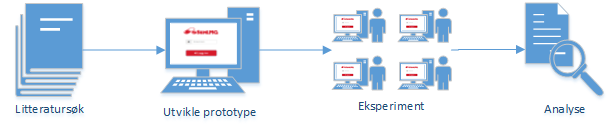
\includegraphics[width=10cm]{images/Arbeidsprosessen}
\caption{Arbeidsprosessen for masteroppgaven}
\label{fig:arbeidsprossen}
\end{center}
\end{figure}
\subsection{Fremdriftsplan}
For å finne rytmen og sikre fremdrift i prosjektet laget vi en fremdriftsplan. En fremdriftsplan skal vise når de forskjellige delene av prosjektet skal utføres og når de skal være ferdig. I vedlegg \ref{vedlegg:milep} ligger fremdriftsplanen. Denne er laget i form av en milepæleplan med et Gantt-skjema og illustrerer tidsplanen for prosjektet. 

Masteroppgave strekte seg på en tidsperiode fra 15.01.2016 til 01.06.2015. Underveis planla vi diverse oppgaver som måtte gjøres både før og etter selve utviklingen. Dette ville være oppgaver som å ha klart design og kravspesifikasjoner for prototypen, levere søknad til \gls{nsd} og analysere resultater av forsøk.
Alt som hadde med selve prototypen å gjøre valgte vi å markere med ekstra fet skrift i milepæleplanen. Dette var oppgaver som primært handlet om leveranser.  Vi valgte å lage et Gantt-skjema (Figur \ref{fig:ganttdiagram}) for å kunne få en bedre visualisering av tidsplanen. Her var det også rom for å bryte opp oppgaver fra milepæleplanen i mer spesifikke oppgaver med frister.
\begin{figure}[H]
\begin{center}
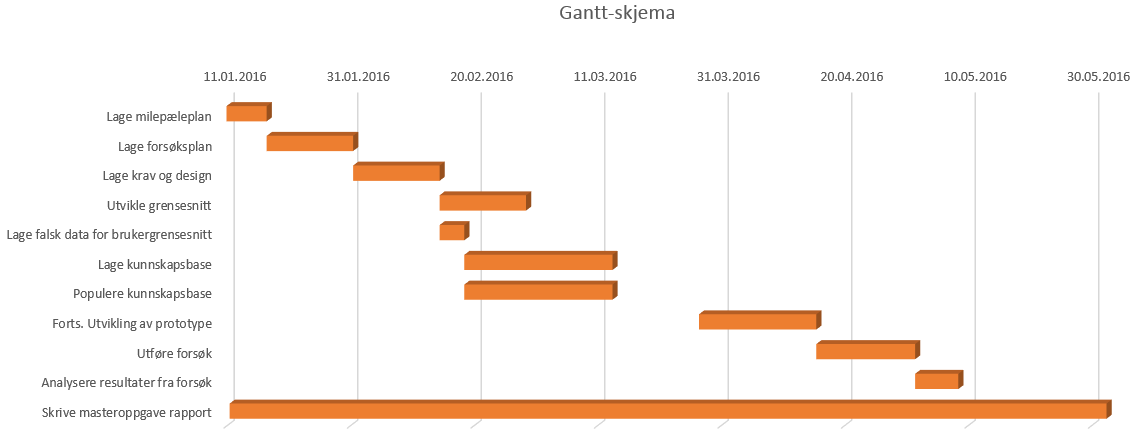
\includegraphics[width=16cm]{images/milep-gant-diagram}
\caption{Gantt-skjema over milepælene}
\label{fig:ganttdiagram}
\end{center}
\end{figure}
I et prosjekt som har en varighet på flere måneder er det essensielt å planlegge oppgaver underveis. Dette ville også være en god måte å unngå missforståelser. Med et Gantt-skjema vil alle være på samme bølgelengde, effektivt allokere og forstå relasjonene mellom oppgavene. Samtidig vil interessenter for prosjektet ha en felles forståelse for hva som er neste steg underveis i prosjektet.
\section{Arbeidsfordeling}

\section{Utvikling av prototypen}
 For å planlegge en prototype er det viktig å definere formålet med prototypen. Formålet med prototypen er å støtte legemiddelgjennomgang med forslag til tiltak for legemidler. For å kunne komme med forslag trengte prototypen å hente en kasuistikk, samstemme legemidler fra kasuistikken og dermed finne tiltak for legemidlene. Figur \ref{fig:formaalsbildeProto} er en konseptuell modell som beskriver hvert formål. Prototypen skulle bli brukt i et eksperiment og trengte derfor å bli utviklet etter dette formålet.
\begin{figure}[H]
\begin{center}

\includegraphics[width=14cm]{images/Formaalsbilde_prototype.png}
\caption{Konseptuell for prototypen}
\label{fig:formaalsbildeProto}
\end{center}
\end{figure}
\subsection{Kravspesifikasjoner}
Kravspesifikasjonen inneholder krav for å kunne bruke en slik prototype i et eksperiment. Et slik eksperiment ville kreve å ha målinger på hva deltakeren klikker på, hvilke tiltak som blir tatt og hvor lang tid deltakeren bruker.
\subsubsection{Brukergrensesnitt}
Da tyngden i prototypen ligger i tiltaksrepresentasjonen var det likevell viktig at prototypen var anvendbar, effektiv og tilfredstillende. Brukergrensesnittet skulle ha høy anvendbarhet slik at deltakere i stor grad kunne utføre de forhåndsbestemte oppgavene i eksperimentet. Den måtte også være effektiv slik at deltakere fort forstår hvordan det fungerer og klarer å navigere seg frem og tilbake på egenhånd. Det ønskes også at deltakere får en tilfredsstillende følelse ved å bruke prototypen.
\subsubsection{Tidsforbruk}
For å kunne bruke prototypen i et eksperiment måtte den måle tiden en deltaker bruker i prototypen under utførelsen av eksperimentet. Tidsforbruket som blir målet ville da kunne fungere som et tidsestimat på hvor lang tid en deltaker bruker på legemiddelgjennomgangen med prototypen.
\subsubsection{Lagring av skjema for legemiddelgjennomgang}
Når legemiddelgjennomgangen er ferdig skal det lagres i en database. Dette vil fungere som et resultat av legemiddelgjennomgangen og kan vurderes av en fagperson. 
\subsubsection{Lagring av klikk}
Lagring av klikk i grensesnittet kunne være et hjelpemiddel for analyse. Hva en person har klikket på kan i stor grad være til hjelp i å forstå hvordan en person har vurdert tiltakene. Prototypen skulle registrere at en deltaker har valgt å bruke tiltakene selv om personen har fjernet tiltaket i etterkant. Tiltakene har en kilde, og denne kilden skulle en deltaker kunne lese. Prototypen måtte derfor også registrere om en deltaker hadde klikket på kilden, noe som ville bety at deltakeren sannsynligvis hadde lest kilden.
\subsubsection{Spørreskjema}
Når deltakere er ferdig med å gjennomføre legemiddelgjennomgangen må systemet videresende deltakeren til et spørreskjema. Det var planlagt å ha et spørreskjema per kasuistikk. Prototypen må derfor kunne skille på kasuistikkene og videresende til riktig spørreskjema. Det måtte være en kobling mellom resultatet av legemiddelgjennomgangen og spørreskjema, derfor må det være et brukernavn for hver deltaker på hver kasuistikk. Dette brukernavnet må også vidersendes til og fylles ut automatisk i spørreskjema.

\subsection{Kasuistikker}
To kasuistikker skulle bli utarbeidet av våre biveiledere. Antallet ville være tilstrekkelig med tanke på at hver enkelt deltager skulle utføre to legemiddelgjennomganger. Kasuistikkene ga oss muligheten til å teste prototypen på ''reelle'' caser uten å bekymre oss om problemer rundt personopplysninger og pasientsikkerhet. Det var viktig at kasuistikkene inneholdte verdier på pasientspesifikk nyrefunksjon, enten i form av Estimert glomerulær filtrasjonshastighet (eGFR) eller utskillelse av kreatinin. Videre var det viktig at kasuistikkene som skulle bli utviklet var så virkelighetsnær som mulig, for å gjøre situasjonen ved bruken SemLMG så reell som mulig. 

\section{Utvikling av kunnskapsbase}
Prototypen krever en kunnskapsbase. Kunnskapsbasen vil ha strukturert informasjon som skal være tilgjengelig å bruke. Kunnskapsbasen vil være i form av en ontologi\ref{bakg:ontologi}

Det finnes ikke én korrekt metodikk for å utvikle en ontologi. I dette kapittelet ønsker vi å diskutere og vurdere en mulig prosess for å utvikle vår ontologi. Denne prosessen vil være en iterativ prosess som vil føre til et godt ontologidesign. Prosessen har vi adaptert fra en brukerveiledning som er skrevet ved Stanford University. \citep{ontology_101}
\subsection{Fastslå domenet og omfanget av ontologien}
Det første steget som må utføres er å definere domenet og omfanget for ontologien. For å gjøre dette vil vi stille oss noen basis spørsmål:
\begin{itemize}
\item Hva er domenet som ontologien skal dekke?
\item Hva er det ontologien skal brukes til?
\item Hvilke spørsmål er det ontologien skal svare på?
\item Hvem vil bruke og vedlikeholde ontologien?
\end{itemize}
Disse spørsmålene kan endre seg under ontologidesignet, men kan hjelpe oss til å avgrense omfanget til modellen vår. For å svare på disse spørsmålene er det naturlig å være i kontakt med interessenter og få en forståelse for hva systemet innebære og levere. Her har vi et godt utgangspunkt da vi har vært i mye kontakt med sektoren, veileder fra NTNU og våre bi-veiledere for masteroppgaven ved Sykehusapoteket i Midt-Norge. \\
En måte å definere omfanget på er å lage seg en liste over kompetansespørsmål. Dette er en liste som vil inneholde spørsmål som en kunnskapsbase skal kunne svare på. Dette er spørsmål som vil kunne fungere som en indikatortest for om ontologien inneholder nok informasjon slik at den kan svare på disse spørsmålene. Det er viktig å merke seg at disse spørsmålene er bare en slags kladd, og trenger ikke å være utfyllende. Før vi starter vår konstruksjon av ontologien vil vi definere disse kompetansespørsmålene for å ha et godt utgangspunkt.

\subsection{Bruk av eksisterende ontologier og informasjonskilder}
Det er nesten alltid lurt å vurdere å bruke eksisterende kilder og sjekke om vi kan raffinere og utvide disse til vårt formål. Dette kan være spesielt viktig om vårt system skal interagere med andre systemer eller vokabular. Det finnes allerede eksisterende ontologier og informasjonskilder som kan ha verdiskapning for oss. DrOn er en ontologi som vi kan ha nytte av å bruke. Om vi ikke bruker ontologien direkte så har DrOn modulære mønstre som vi kan adaptere inn i vår ontologi. Femstjerners FEST er også et interessant prosjekt og vi kommer til å ha kontakt med Statens Legemiddelverk både for tilgang til informasjonskilder og høre hvordan utviklingen går. ICD's internasjonale standard for felles terminologi og klassifisering av sykdommer er noe å betrakte. I vårt scenario ser vi på nyrefunksjonen. Ved å klassifisere sykdommen kan vi ved en senere anledning utvide kunnskapsbasen og rangere sykdommer. Et annen kilde for klassifikasjon er ATC. Dette kodeverket kan vi bruke for å gjøre effektive spørringer på hvilket organ legemidler påvirker samt virkemåte og egenskaper.

\subsection{Liste opp viktige begreper i ontologien}
Det kan være nyttig å liste opp viktige begreper som kan bli brukt i ontologien og i domenet. I vårt domenet ville det være naturlig å se på hva en medisin inneholder. Dette kan være begreper som virkestoff, dosering, interaksjon, indikasjon og bivirkning. Det kan også være nyttig å lage seg på begrepsapparatet innen farmasi. Når man skal liste opp slike begreper er det viktig å ikke tenke på overlapp eller hvilke relasjoner de har til hverandre. Det viktigste er å få listet de opp slik at de kan anvendes og moduleres senere.

\subsection{Definere klasser og klassehierarki}
Hvordan en tenker for å komme frem til klasser og klassehierarki er avhengig av et personlig synspunkt, og det er ingen metode som er bedre enn noen andre. Under vil vi liste opp tre mulige utviklingsprosesser for å oppnå et best mulig design av klasser:
\begin{itemize}
\item \textbf{Top-down} starter med det mest generelle konseptet i et domene, hvor du senere legger til videre spesialiseringer av konseptet. Man kan se for seg konseptet menneske. Hvor man kunne startet med å konstruere det mest generelle mennesket, og etterhvert spesialiserer hvilke kjønn eller raser som finnes.
\item \textbf{Bottom-up} starter med å definere de mest spesifikke klassene først, altså løvnodene i et typisk node-tre, og dermed grupperer disse spesifikke klassene i mer generelle klasser. Dette blir da motsatt tankegang av top-down.
\item En \textbf{kombinasjon} av disse to utviklingsprosessene er kanskje den mest vanligste måten å tenke på. Man starter med å definere det mest fremtredende først, dermed spesialiserer man superklasser og subklasser som tilhører denne. \\

\end{itemize}
Som sagt er dette personlig, og hvis en utvikler har et systematisk top-down syn på domenet, vil det være enklere å bruke top-down tilnærmingen. Kombinasjonprosessen er ofte enklere for mange ontologi utviklere. Dette kan være fordi konsepter som er fremtredende ofte er "midt-i", og disse er ofte mer deskriptive konseptene i et domene. \\

Det finnes ikke bare et eneste korrekt klassehierarkiet for et gitt domene. Hierarkiet avhenger av forskjellig bruk av ontologien, hvor detaljert den skal være for, personlige preferanser og noen ganger avhengigheter for å være kompatibelt med andre modeller. Det finnes flere retningslinjer for å sørge for at hierarkiet er mest mulig korrekt. Under konstruksjon av vår ontologi ønsker vi å ta hensyn til følgende retningslinjer: \\
\begin{itemize}
\item \textbf{Unngå klassesykluser:} En burde alltid unngå klassesykluser. En klassesyklus er typisk når du har en klasse A som har en subklasse B, og denne subklassen B er superklassen til klasse A. En slik situasjon tilsier at klasse A og klasse B er ekvivalent (alle instanser av A er instanser av B, og alle instanser av B er instanser av A). 
\item \textbf{Klasser og navn:} Det er viktig å skille på en klasse og navnet til en klasse. Navnet til en klasse kan endre seg hvis vi endrer terminologien, men begrepet er fortsatt et objekt i den virkelige verden. Et eksempel er hvis vi har et konsept som vi kaller \textit{Medisin}, men vi velger å endre navnet til \textit{Legemiddel} istedet. Klassen skal fortsatt representerer det samme konseptet, og alle tilhørligheter til konseptet skal bestå uten komplikasjoner.
\item \textbf{Entall/flertall versjoner av samme konsept:} En typisk feil å er å inkludere både entall og flertall versjoner av samme konsept. For eksempel ville det vært feil å definere en klasse \textit{Medisiner} og en subklasse \textit{Medisin}. Den beste måten å unngå slike feil er å forholde seg til enten entall eller flertalls navnekonvensjoner.
\end{itemize}
Disse er bare et fåtall av de retningslinjene som blir presentert i brukerveilederen som er utviklet på Stanford, men vi synes de omtalte retningslinjene er de mest sentrale for vårt prosjekt. \citep{ontology_101} Noen av de andre retningslinjene som blir presentert går på når en ny klasse bør bli introdusert og hvor mange subklasser er for mye eller for lite. Dette er vanlige problemstillinger når man holder på med datarelatert modellering, og veldig vanlig å ha i bakhodet under konstruksjon. Vi ønsker ikke å gå mer i detalj om dette i vår rapport.  

\subsection{Definere egenskaper til klasser}
Så langt har vi listet opp hvordan man går frem for å lage klasser og klassehierarkier. Klasser alene er ikke nok til å svare på kompetansespørsmålene som vi lister opp. For dette trengs det å defineres interne strukturer til objektene. Dette kalles egenskaper (properties), og vil hjelpe oss med å si noe mer om konseptene og relasjonene mellom dem.
Generelt sett finnes det flere typer objektegenskaper som kan bli egenskaper i en ontologi:
\begin{itemize}
\item Indre (intrinsic) egenskaper er verdier som er en naturlig del av et konsept. Dette kan for eksempel være øyenfargen på et menneske.
\item Utvendige (extrinsic) egenskaper er verdier som ikke er en naturlig del av et konsept. Dette er egenskaper som kommer fra "utsiden" av et konsept. Dette kan for eksempel være navnet på et menneske.
\item Hvis et konsept har en struktur er det naturlig å dele opp konseptet i deler. Dette er også egenskaper til et konsept, og disse delene kan være fysisk eller abstrakte elementer ved et konsept.
\item Forholdet til andre individer, dette er relasjoner mellom individer mellom medlemmer av klasser eller andre elementer.
\end{itemize}
Ettersom egenskaper arves på samme måte som objekt orientert arv, burde egenskaper tilhøre den mest generelle klassen i et klassehierarki. For eksempel burde øyenfarge være en del av klassen menneske, slik at subklassene mann og kvinne arver øyenfarge fra sin superklasse menneske. En mann og en kvinne arver øyenfarge fordi de begge er mennesker.

\subsection{Definere fasetter til egenskaper}
Egenskapene kan ha flere fasetter. Dette kan for eksempel være hvilke verdityper en egenskaper har eller hvor mange verdier som er lov (kardinalitet). Vi ønsker å liste opp noen fasetter som kan være viktige å tenke igjennom for å oppnå best mulig design: \\

\subsubsection{Kardinalitet}
Egenskapenes kardinalitet defineres som hvor mange verdier en egenskap kan ha. Noen systemer skiller mellom enkel (høyst en) og multippel (ethvert antall) kardinalitet. Et eksempel på dette kan være nesen og øyene til et menneske. Ved bruk av enkel kardinalitet for nesen vil et menneske kun ha en nese, mens ved bruk av multippel kardinalitet for øynene vil et menneske kunne ha to øyner. \\
Noen systemer tilater å a et maksimum og minimum kardinalitet på egenskaper. Dette er for å definere verdiene mer presist. Minimum kardinalitet av \textit{N} vil bety at en egenskap må ha minst \textit{N} verdier, mens maksimum kardinalitet på \textit{M} vil bety at en egenskap kan ha maks \textit{M} verdier. \\

\subsubsection{Relasjonsmønstre til en egenskap}
Ved konstruksjon av egenskaper må det vurderes om egenskapens relasjoner skal ha restriksjoner som sier noe om relasjonsmønsterert til egenskapen. Disse restriksjonene blir uttrykt ved å bruke domain og range attributtene. Restriksjonene vil si noe om hvilke klasser en egenskap tilhører. Et utsagn om at to individer har en relasjon til hverandre via en spesiell egenskap kan bære med seg ekstra implisitt informasjon om disse individene og konklusjoner kan trekkes.





\chapter{Gjennomføring}
I dette kapittelet ønsker vi å utrede hvordan vi gjennomførte hvert steg av forskningsplanen Kapittel \ref{chap:fremgangsmate}. De påfølgende underkapitlene er litteratursøk, utvikling av prototype og gjennomføring av eksperimentet.
\section{Litteratursøk}
Et litteratursøk ble foretatt for å se hva som er gjort tidligere i vårt problemdomene. Litteratursøk innebærer å finne kunnskap tilgjengelig i forskjellige databaser, for å kritisk gjennomgå disse. Siden vårt problemdomene går inn på flere fagområder, valgte vi å dele inn litteratursøket i flere deler. Siden planen er å utvikle et støtteverktøy med semantisk webteknologi der brukeren utfører legemiddelgjennomgang, ble inndelingen følgende: 1)Hvilken informasjon trenger helsepersonnell ved legemiddelgjennomgang 2)Forsøk på beslutningsstøtte til legemiddelgjennomgang eller forskrivning av legemidler 3)Bruk av semantisk webteknologi for modellering av legemiddelinformasjon. Databasene vi tok i bruk for å finne litteratur for disse temaene var hovedsakelig PubMed og Google Scholar. IEEE Xplore, UpToDate og Tidsskriftet.no ble brukt i mindre grad.              
\label{chap:gjenomf_litteratursok}
\subsection{Behov for legemiddelinformasjon}
Vår prototype skal forsøke å gi kliniske farmasøyter tilstrekkelig informasjon om legemidler. Derfor har vi foretatt et litteratursøk for å se på helsepersonells behov for legemiddelinformasjon ved behandling av pasienter.

Hvilke faktorer som påvirker helsepersonells valg av kilder er uklart. I en hektisk arbeidshverdag der tiden er knapp viser det seg at man i primærhelsetjenesten setter effektivitet høyt når det gjelder valg av kilder \citep{Cook_Sorensen_2013}. Med effektivitet menes at kilden har svaret på det kliniske spørsmålet de lurer på, og at det er enkelt å finne fram til svaret. Hvor raskt man kan finne svaret er avhengig av struktur av kilden, søkefunksjonalitet, lengde på innhold og kjennskap til bruken. Videre er det andre faktorer som spiller inn på valg av kilder som inkluderer tett integrasjon i arbeidsflyten, kredibilitet, kontaktinfo til ekspert, rettet mot kliniske spørsmål, oversettelse til lokale behandlingsprosesser og mulighet for pasientopplæring. Ingen av kildene nevnt, blant annet PubMed, MEDLINE og UpToDate, dekker alle behovene.

Fastleger har behov for legemiddelinformasjon til støtte under forskrivning, men informasjonen gitt av beslutningsstøttesystemer møter ofte ikke deres behov\citep{Rahmner_Eiermann_2012}. Interaksjoner, bivirkninger, allergier og hypersensitivitet, aldersrelatert dosering og indikasjoner var noen av informasjonsbehovene som ble nevnt. Flere rapporterte eksempelvis at interaksjoner var oppgitt i beslutningsstøttesystemet i bruk, men at for mye informasjon gjorde at advarslene ble sett på som mindre viktige eller ignorert.  Ved aldersrelatert dosering var det ønske om at et system beregnet glomerulær filtrasjonsrate, slik at en kan enklere foreta riktige dosejusteringer for pasienter med nedsatt nyrefunksjon. 
\subsection{Klinisk beslutningsstøtte}
Prototypen er et forsøk på å undersøke hvorvidt støttesystem kan hjelpe kliniske farmasøyter i å utføre legemiddelgjennomganger. Et litteratursøk er derfor foretatt for å se på tidligere forskning omkring beslutningsstøtte for legemiddelgjennomgang og forskrivning av legemidler.
\subsubsection{STRIP}\label{STRIP}
Systematic Tool to Reduce Inappropiate Prescribing(STRIP) er et klinisk beslutningsstøttesystem for legemiddelgjennomgang utviklet i Nederland \citep{STRIP}. Verktøyet er beregnet for bruk i polyfarmasi, altså for pasienter som benytter flere medikamenter og i større doser enn ønskelig. STRIP tar i bruk og kombinerer START og STOPP-kriteriene for å gi ut en farmakoterapeutisk analyse som blant annet inkluderer sjekker for dosejustering, overbehandling og underbehandling, bivirkninger, interaksjoner, dosefrekvens og inntaksmåte. I tillegg til denne analysen tar STRIP også hensyn til pasientens preferanser og legemiddelhistorikk. Et eksperimentet viste at legemiddelgjennomgangen ble mer korrekt, altså at det ble gjort flere riktige avgjørelser og færre uriktige. På en annen side brukte de signifikant lengre tid på legemiddelgjennomgangen. Brukergrensesnittet var lite tilfredstillende i bruk. 

\subsubsection{SMART}
En nylig foretatt studie så på muligheten til å bedre legemiddelbehandlingen hos geriatrikere ved å implementere Beers kriterier og beregning av glomerulær filtrasjonsrate i et eksisterende EPJ-system\citep{SMART}. Denne beslutningsstøtten ble kalt Seniors Medication Alert and Review Technologies(SMART). SMART ga beslutningsstøtte enten passivt i form av meldinger i pasientjournalen(passiv støtte) eller advarsler ved dokumentering av legemidler(aktiv støtte). Denne støtten kunne avdekke uhensiktsmessige legemidler, nedsatt glomerulær filtrasjonsrate(GFR) samt dosejusteringer. GFR ble beregnet ut i fra høyde, vekt og kreatinin-nivåer klinikerne selv skrev inn i systemet. Hver enkelt anbefaling hadde en indikator som viste styrken på anbefalingen og  kvaliteten på evidens, samt lenker til læringsressurser og oppsummeringen av evidensen. Studien viste at klinikerne var enige om at SMART var tilfredstillende i bruk uten å legge store hindringer i arbeidsflyten. Advarslene ble brukt som læringsverktøy og benyttet som evidensbasert støtte ved beslutningstaking. Videre mente klinikerne at SMART styrket, og i noen tilfeller endret deres kliniske beslutning.
\subsubsection{Renal beslutningsstøtte i Janus pasientjournal}
Janusinfo er et pasientjournalsystem med tilhørende verktøy i Sverige.
\ot{Si noe om dette Janus pasientjournalsystemet?}

The Renal Button er navnet på en pilot av et beslutningsstøttesystem ment for å støtte dosering av legemidler basert på en estimering pasienters utskillelse av kreatinin\citep{Hellden_Al-Aieshy_2015}. Renal utskillelse av legemidler er korrelert til utskillelse av kreatinin. Beslutningsstøtten ble implementert i Janus pasientjournalsystem. The Renal Button ga støtte svar på 1)Er legemiddelet hensiktsmessig og hvilken dosering,2)Risikoen for å ikke tilpasse dosen etter evne til utskillelse av kreatinin. Hvert forslag inkluderte en større tekstlig beskrivelse samt referering til kilder. Estimasjon av kreatininnivå ble beregnet ved å bruke pasientdata som alder, kroppsvekt, kjønn og P-kreatinin hentet fra informasjonen i EPJ-systemet. En evaluering av systemet undersøkte pilotens nytteverdi og brukernes oppfattelse av brukergrensesnittet. Samtidig ble antall pasienter med estimert utskillelse av kreatinin før og etter bruk av systemet målt. Antall pasienter med estimert utskillelse av kreatinin økte med 1.6 etter bruk av systemet.

Et annet pilotprosjekt utviklet et beslutningsstøttesystem for forskrivning av legemidler til pasienter med nedsatt nyrefunksjon\citep{Shemeikka_Bastholm-Rahmner_2015}. Dette ble også implementert i Janus pasientjournalsystem. Istedenfor å estimere utskillelse av kreatinin, ble estimert glomerulær filtrasjonsrate(eGFR) brukt for dosejustering etter pasientens nyrefunksjon. Verdien av eGFR ble vist sammen med legemiddellisten. Systemet ga anbefalinger for dose, som var klassifisert etter hvorvidt nedsatt nyrefunksjon påvirket pasientens opptak av legemiddelet. Evaluering av beslutningsstøttesystemet viste at deltagerne fikk økt forståelse for dosering, og at bruken av støtten var tidsbesparende.   

\subsection{Semantisk modellering av legemiddelkunnskap}
Prototypen skal bruke semantisk webteknologi for å modellere legemiddelkunnskap. Denne seksjonen utgreier om tidligere arbeid og forskning på modellering av legemiddelkunnskap og tilhørende informasjon med semantiske webteknologier.

\subsubsection{Modellering av farmakogenetikk}
En studie beskriver et pilotprosjekt der målet var å bygge en semantisk modell av farmakogenetisk informasjon knyttet til legemidler\citep{Boyce_Freimuth_2013}. Formålet med å bygge en slik modell var å bruke strukturert farmakogenetisk informasjon som beslutningsstøtte i klinisk-og-translasjonsforskning. Beslutningsstøtten skulle svare på spesifikke kliniske spørsmål, f.eks: For pasient med genotype x, finn anbefaling for et legemiddel, inkludert doseendringer og eventuelt alternative legemidler. 

\subsubsection{Open PHACTS}
Open pharmacological concepts triple store (open PHACTS) er en platform ment for å assistere funn av potensielle legemidler. Ved bruk av semantisk webteknologi, er datagrunnlaget satt sammen av flere heterogene informasjonskilder forskere innenfor farmakologi, medisin og bioteknologi allerede bruker. Disse kildene inneholder detaljert farmakologisk informasjon om legemidler, stoffer, molekylære forbindelser, kjemisk strukturer, enzymer, gener, reaksjonsveier og mer. Tjenesten brukes enten som et webgrensesnitt eller ved bruk av et API\citep{open_phacts_explorer}. En studie har sett på hvordan Open PHACTS kan støtte funn av potensielle legemidler\citep{Ratnam_2014}. Videre konkluderer studien med at Open PHACTS løser tidligere integrasjonsproblemer den enkelte hadde i form av lisensiering, formattering og søk.

\subsubsection{DrOn}
\gls{dron} er en modulær ontologi for legemiddel-produkter utviklet med semantiske teknologier. Den innehar informasjon om ingredienser og biologisk aktivitet med utgangspunkt i legemidler som selges i USA \citep{dron_2013}. Ontologien bruker RxNorm som dets eksterne hovedkilde, som er en medisinsk terminologi som inneholder alle legemidler til salgs i USA. Disse legemidlene er kartlagt opp mot ChEBI-klasser. \gls{chebi} er en database og ontologi som inneholder molekylære entiteter. Resultat av dette er at en kan resonnere mellom legemidler med tilhørende ingredienser og biologiske aktivitet. 

For å lage denne ontologien minet de data fra utgivelser av RxNorm. Dette ble gjort ved å laste ned råfilene, omforme dataene for å deretter importere dette i en relasjonsdatabase ved hjelp av et skript som er tilgjengelig. Så ble RxNorm-entiteter kartlagt opp mot ChEBI-klasser ved hjelp av en konsollapplikasjon som sammenlignet etiketter av ingredienser i RxNorm med klasseannoteringer i \gls{chebi}. Deretter ble den normaliserte databasen oversatt til en OWL-artefakt. 

\gls{dron} er modulært, slik at klasser fra hver kilde er serialisert i separate moduler som igjen er konsumert(del av..) av klasser som er manuelt utarbeidet på et høyere nivå i en modul med termer som «klinisk rolle», «tablett», «kapsel» med mer. På denne måten kan en enkelt bruke deler av ontologien i tillegg til at videreutvikling vil være enklere. 

Denne ontologien inneholder mye informasjon om legemidler, og kan spille en viktig rolle i utviklingen av vårt system. Framgangsmåten deres kan være nyttig for oss, selv om vi velger å ikke ta i bruk \gls{dron}. Hvis vi går for å bruke \gls{dron} på en eller annen måte, er det visse aspekter med ontologien vi må ta stilling til. Den største problemstillingen vil nok være å bruke denne ontologien i norsk sammenheng. Er det mulig å koble amerikanske legemidler opp mot legemidler til salgs i Norge? 
\section{Utvikling av prototype}
I følgende underkapitler vil vi legge frem bakgrunnen og oversikten, totaldesign og dermed bryte opp totalen for å legge frem hvordan vi har designet de forskjellige delene. Vi vil også vise en liten demostrasjon av hvordan prototypen så ut og hvordan vi gjennomførte forsøket med prototypen. Dette underkapitelet vil være teknisk og vil vise teknologiske valg som ble tatt underveis.
\label{chap:gjenomf_utviklingavprototype}
\subsection{Bakgrunn}

Semantisk legemiddelgjennomgang (SemLMG) var en prototype som ble utviklet hvor formålet var et støtteverktøy under legemiddelgjennomgang. Prototypen skulle gi brukeren relevant og enkelt tilgjengelige tiltak for legemidler for å se om den kunne gi et bedre beslutningsgrunnlag. For å kunne realisere prototypen ville prototypen foreslå tiltak for en bestemt kategori under legemiddelgjennomgangen. Kategorien heter ''Legemiddel ikke tilpasset pasient''. Denne kategorien går på tiltak for nyre- og leverfunksjoner. Tiltakene som prototypen presenterte for brukeren var tiltak ved nedsatt nyrefunksjon.

En bruker skal kunne lese en kasuistikk, få en oversiktlig liste over legemidler og til slutt få opp et skjema som brukes til å utføre en legemiddelgjennomgang. Prototypen var designet slik at noen varianter av kasuistikkene var med eller uten foreslåtte tiltak. Prototypen skulle brukes når og hvor som helst i en bestemt tidsperiode.

%Brukere av prototypen var kliniske farmasøyter som skulle lese en kasuistikk, observere at en samstemt liste blir laget og dermed utføre en legemiddelgjennomgang. Utførelsen av legemiddelgjennomgangen skulle utføres på vanlig vis med vår prototype. Med vanlig vis mener vi at brukerene skulle gjøre legemiddelgjennomgangen så likt virkeligheten som mulig. Dette vil bety at farmasøytene brukte eksterne kilder for å foreslå tiltak. Prototypen var designet slik at noen varianter av kasuistikkene var med eller uten foreslåtte tiltak. For å kunne måle hvor lang tid brukerene bruker under de forskjellige stegene av prototypen ble det gjort tidsmåling i hvert steg. Prototypen var ønsket å kunne brukes når og hvor som helst i en bestemt tidsperiode.
\subsection{Use-case diagram}
Under utvikling av prototypen var det viktig å ha definert en rolle og handlingene mellom rollen og systemet. For å holde oversikt og fokus modellerte vi et use-case diagram (Figur \ref{fig:ucd}
\begin{figure}[H]
\centering
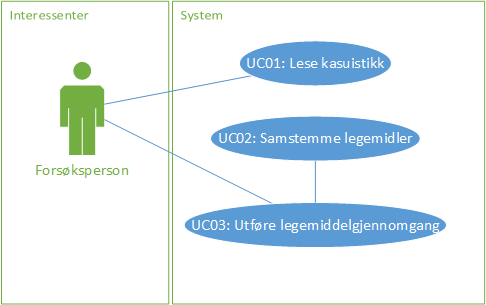
\includegraphics[width=14cm]{images/ucd.png}
\caption{Use-case diagram}
\label{fig:ucd}
\end{figure}
\subsubsection{UC01: Lese kasuistikk}
En forsøksperson skulle kunne lese en kasuistikk. Denne kasuistikken skulle være så reel som mulig og gi utslag for beslutningsstøtten i systemet. Dette vil si at kasuistikken måtte inneholde momenter(overlapp i medisiner, dosefeil, interaksjoner,lab-målinger etc.) som beslutningsstøtten kan fange opp å komme med forslag for. kasuistikken skulle bare være lesbar og forsøkspersonen skulle ikke kunne endre på kasuistikken selv. 
\subsubsection{UC02: Samstemme legemidler}
Systemet måtte samstemme legemiddler. Dette var ikke en use-case som forsøkspersonen skulle utføre selv, men heller observere resultatet av at det skjer automatisk i systemet. En samstemt liste over legemiddler var nødvendig for å kunne utføre legemiddelgjennomgangen og for at systemet skulle klare å lage en foreslått tiltaksliste.
\subsubsection{UC03: Utføre legemiddelgjennomgang}
En forsøksperson skulle kunne utføre en legemiddelgjenomgang. Denne legemiddelgjenomgangen burde være så lik virkeligheten som mulig. Et tiltaksskjema måtte være representert med kategorier som er kjent for forsøkspersonen. For halvparten av brukerne ville en liste med foreslåtte tiltak være tilgjengelig under utførelsen av legemiddelgjennomgangen.
\subsection{Forutsetninger og avhengigheter}
\subsubsection{Forutsetninger}
Forsøkspersonene var kjent med hvordan legemiddelgjennomgang utføres på klinikk i dag. Tiltaksskjema som presenteres når en forsøksperson utfører legemiddelgjennomgang i systemet må være kjent fra før.
\subsubsection{Avhengigheter}
For å utføre samstemming av legemiddler falt valget på å gjenbruke et tidligere prosjekt, MedExt, som er startet ved NTNU.\citep{rost2014development} MedExt var derfor en avhengighet for at systemet skal kunne fungere optimalt. Utgangspunktet for besluttningstøtten var kasuistikken, og vi var dermed avhengig av at kasuistikkene var gyldige for kunnskapsmodellen og på et format som ville fungere med MedExt.

\subsection{Totaldesign}
Designarkitekturen for hele systemet er representert i figur \ref{fig:designview}.
\begin{figure}[H]
\centering
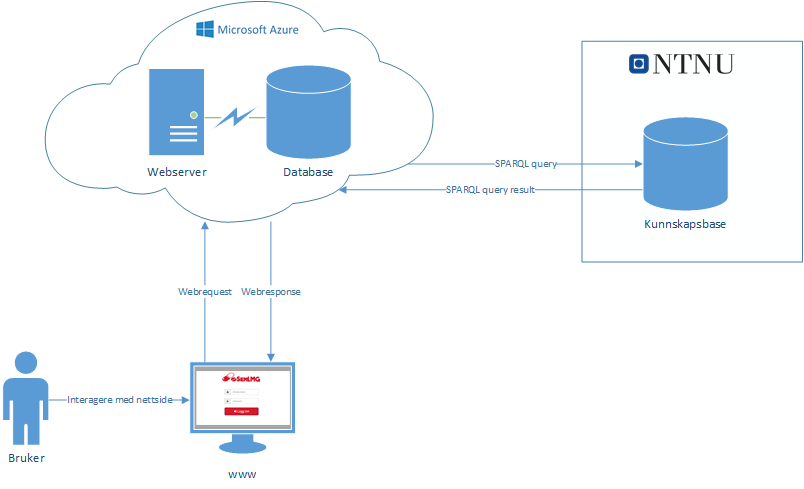
\includegraphics[width=14cm]{images/designview.png}
\caption{Designarkitekturen til SemLMG}
\label{fig:designview}
\end{figure}
Dette er et teknisk oversiktsbilde over hvordan vi ønsket å designe systemet. Brukeren skulle interagere med et webgrensesnitt som kommuniserer med et miljø som eksisterte i Microsoft Azure (skytjeneste). I skyen skulle web-forespørsler håndteres og kontrolleres for å dermed sende web-svar slik at webgrensesnittet ble oppdatert riktig og presentert for brukeren. Når brukeren sendte web-forespørsler hvor skyen trengte å kommunisere med kunnskapsbasen ble det laget \gls{sparql} spørringer til en tjener ved NTNU. Denne tjeneren skulle levere kunnskap om legemiddelgjennomgang og sende dette tilbake som \gls{sparql} resultat som måtte håndteres i skyen og dermed oppdatere webgrensesnittet.
\subsection{Teknologivalg}
I figur \ref{fig:designviewmedteknologi} har vi utvidet designarkitekturen med teknologi og vi ønsker å legge frem for valg av teknologien.
\begin{figure}[H]
\centering
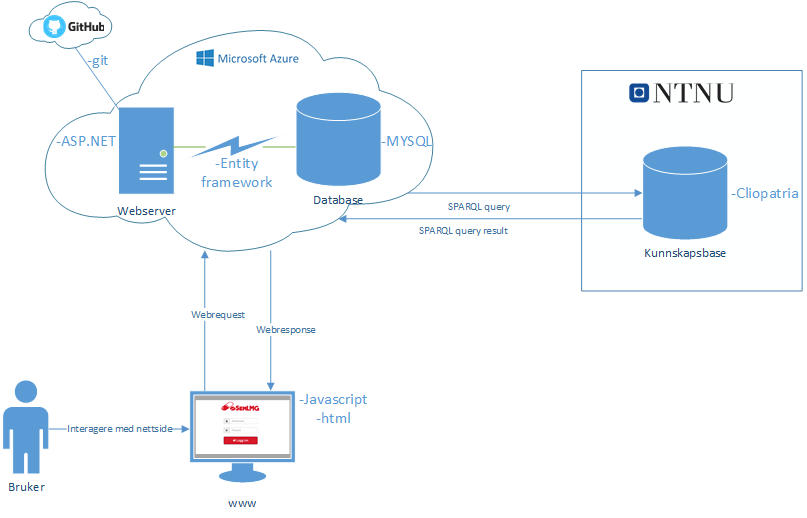
\includegraphics[width=14cm]{images/DesignViewMedTeknologi.png}
\caption{Design perspektivet til SemLMG}
\label{fig:designviewmedteknologi}
\end{figure}
\subsubsection{Webgrensesnitt}

Behovet for å ha et system som kunne være fritt tilgjengelig hvor og når som helst var den høyeste motivasjonen for å utvikle et webgrensesnitt. Etter samtale med biveiledere virket det mest sannsynlig at forsøkspersonene kom til å utføre forsøket på ulike tider i løpet av forsøksuken. Vi ønsket også at det skulle være enkelt for oss å deployere prosjektet. Fordelen var at vi unngikk behovet for å installere noe som helst og at prototypen kunne brukes når og hvor som helst. Grunnet valg av hostingteknologi ble webgrensesnittet bygget opp av Javascript og Html.
\begin{figure}[H]
\centering
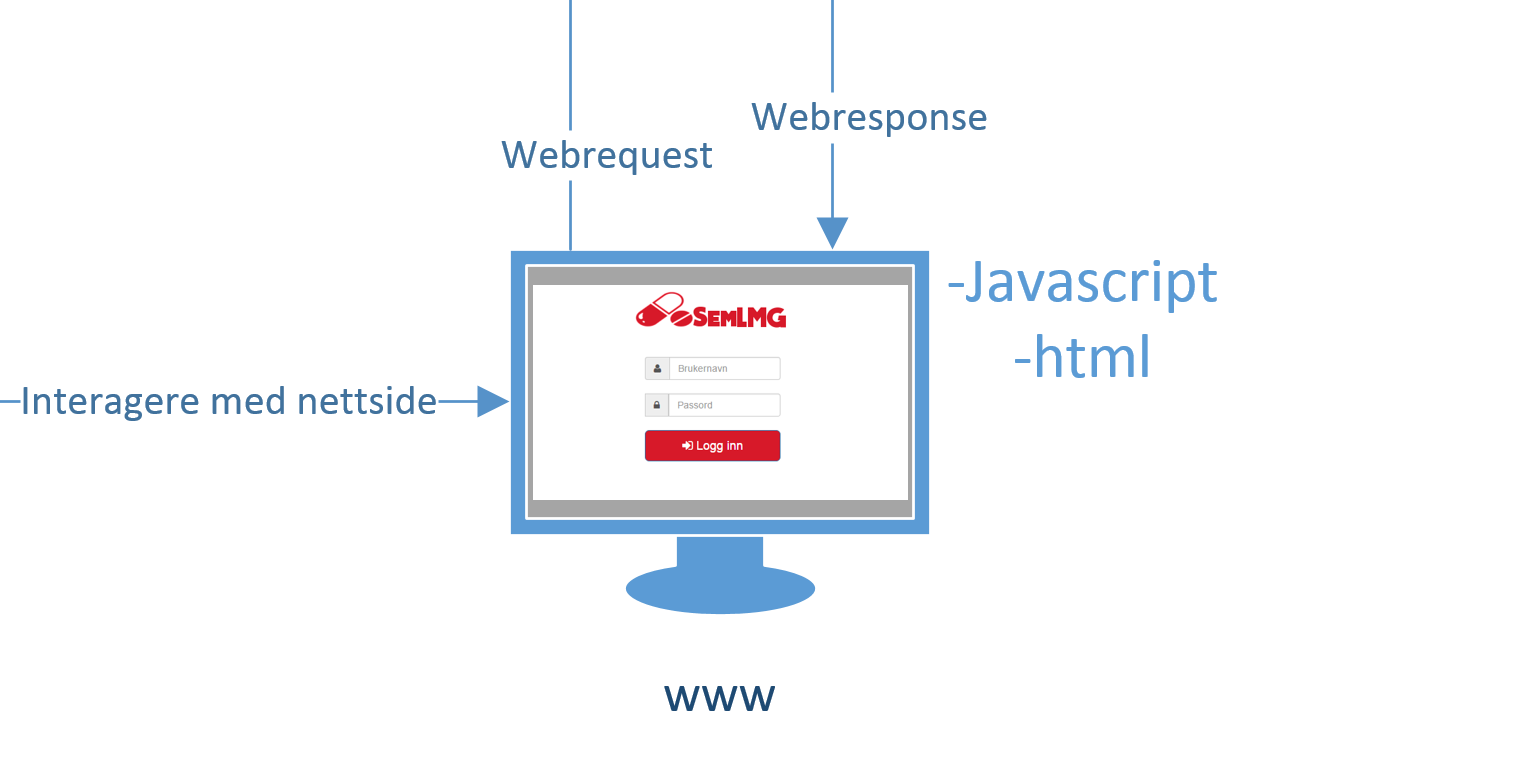
\includegraphics[width=10cm]{images/www}
\caption{Webgrensesnittets teknologi i SemLMG}
\label{fig:webui}
\end{figure}

\subsubsection{Microsoft Azure for hosting}
Oppdagelsen av Azure som hostingpartner kom av at vi lå merke til at studenter ved NTNU har studentlisens på Azure. Vi ble da nysgjerrig på hvordan dette virket og ville prøve oss frem. Azure leverer akkurat det vi trenger for vårt formål og er enkelt å sette opp. I Azure kan vi deployere en eller flere web applikasjoner, opprette database, bruke Azures egne domener og samtidig ha full oversikt over trafikk.
\begin{figure}[H]
\centering
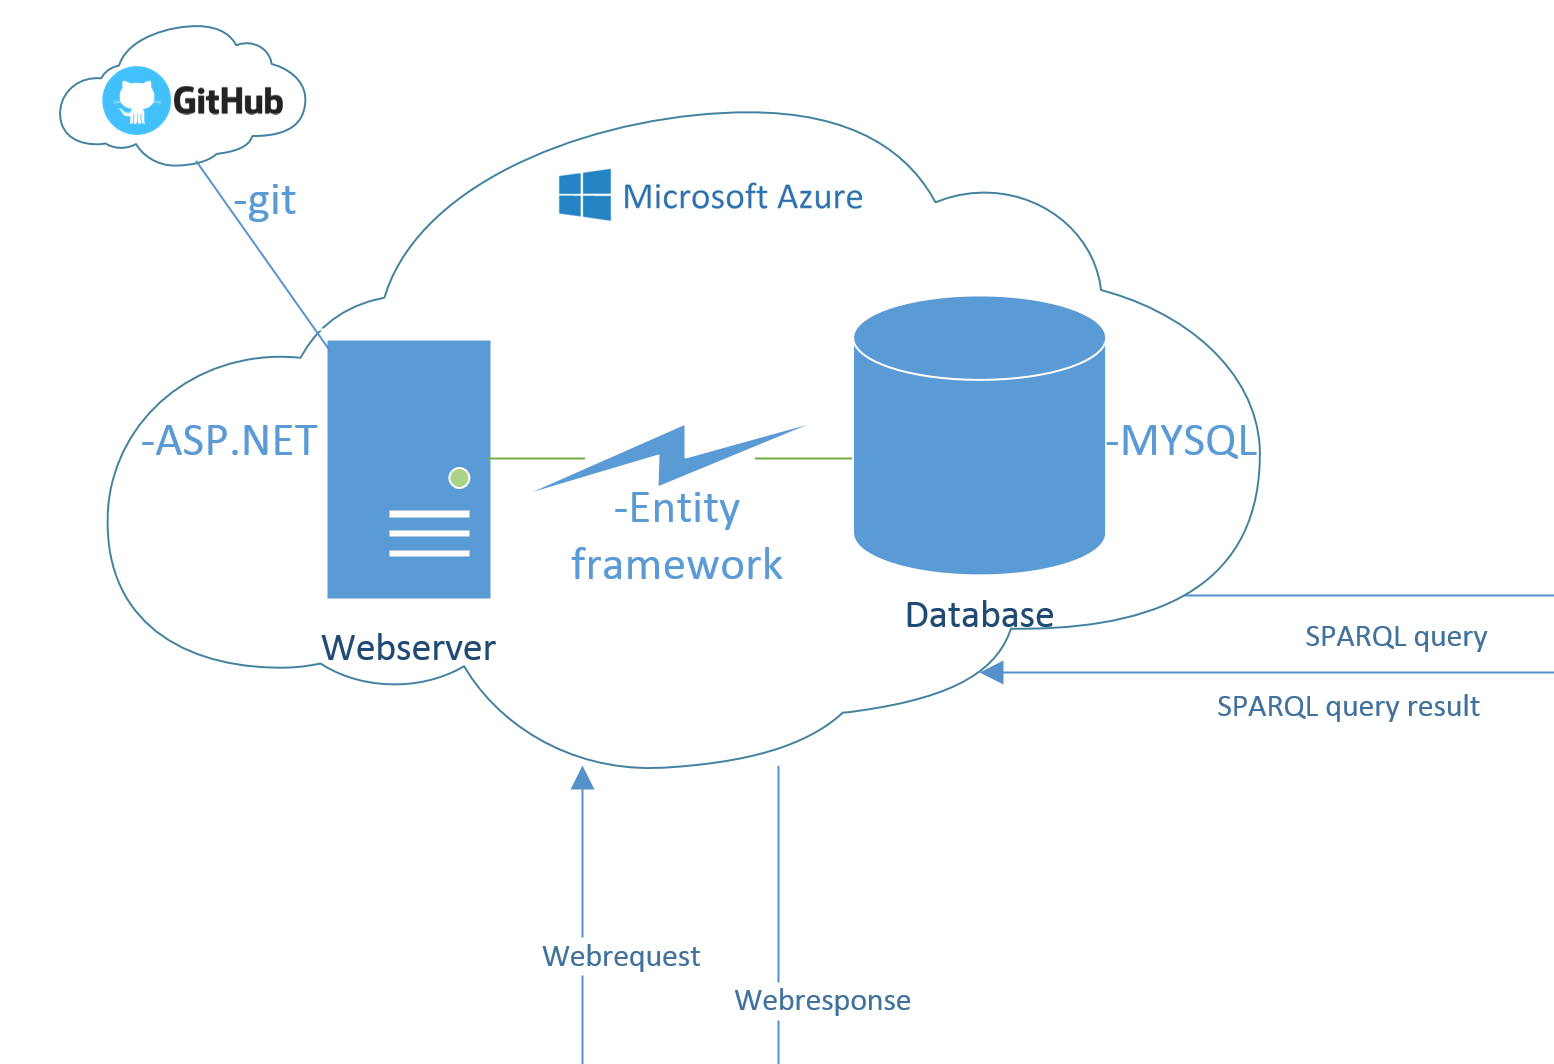
\includegraphics[width=10cm]{images/sky}
\caption{Azure-skytjeneste i SemLMG}
\label{fig:sky}
\end{figure}
\subsubsection{.NET som utviklingsplatform}
Grunnlaget for å utvikle under .NET platformen kom av at alle i mastergruppen hadde erfaring med dette og kommer til å jobbe på samme platform etter masteroppgave. Når det ble avtalt at vi skulle lage et webgrensesnitt tok vi også beslutningen om å utvikle dette under ASP.NET platformen. I ettertid var dette et godt valgt da MedExt-systemet var tilgjengelig i C\#, noe som førte til at integrasjonsprosessen ble enklere.
\subsubsection{Webserver}
Webserveren deployerte som sagt et ASP.NET prosjekt. Dette prosjektet var utviklet ved bruk av MVC-prinsippet (forklart nærmere i MVC-prinsippet i kap. \ref{chap:mvc}) og kommuniserte med en MYSQL database ved bruk av Entity-Framework rammeverket. Webserveren håndterte web-forespørsler ved å sende web-svar for å oppdatere riktig webgrensesnitt. Hvis brukeren sendte web-forespørsler som hadde behov for å  lagre i databasen vil den bruke Entity-Framework til å lagre i riktig tabell. Hvis brukeren sendte web-forespørsler som krevde kompetansen fra kunnskapsbasen ville den spørre kunnskapsbasen og oppdatere grensesnitt med svar fra kunnskapsbasen. Mer om designet til webapplikasjonen i kap \ref{chap:webapp}.
\subsubsection{Database}
For å kunne ha kasuistikker og resultater fra forsøket hadde vi behov for en database å kunne lagre i. Valget falt dermed på å sette opp en MYSQL database i Azure som webserveren har direkte tilgang til. Mer om designet til databasen i kap \ref{chap:db}.
\subsubsection{GIT som versjonskontrollsystem}
Hele mastergruppen har erfaring med Git og det ble derfor naturlig å bruke dette. Som studenter ved NTNU har vi studentlisens på Github som gjør at vi kan holde prosjektet vårt lukket som privat prosjekt. Azure kommuniserer godt med Github, og vi fant etterhvert ut at vi kunne deployere prosjektet vårt kontinuerlig fra Github. For å deployere leser Azure fra en bestemt Branch i et Github repository og deployere hva enn det må være der. Azure har også fine loggmuligheter og vi kan se om vi har noen feil i Branchen vår når den prøver å bygge prosjektet før deployering.

\subsubsection{Kunnskapsbase}
Ved NTNU står det en tjener som fungerer som en grafdatabase (tripplestore).Denne fikk vi erfaring med våren 2015 hvor vi hadde et prosjekt i emnet Web intelligens. Vi ønsket derfor å fortsette å bruke denne tjeneren som et endepunkt for vår kunnskapsbase. Teknologien som ligger i bunn for å kunne få en grafdatabase opp å gå er Cliopatria. Mer om designet til kunnskapsbasen i kap \ref{chap:kunnskapsbasedesign}.
\begin{figure}[H]
\centering
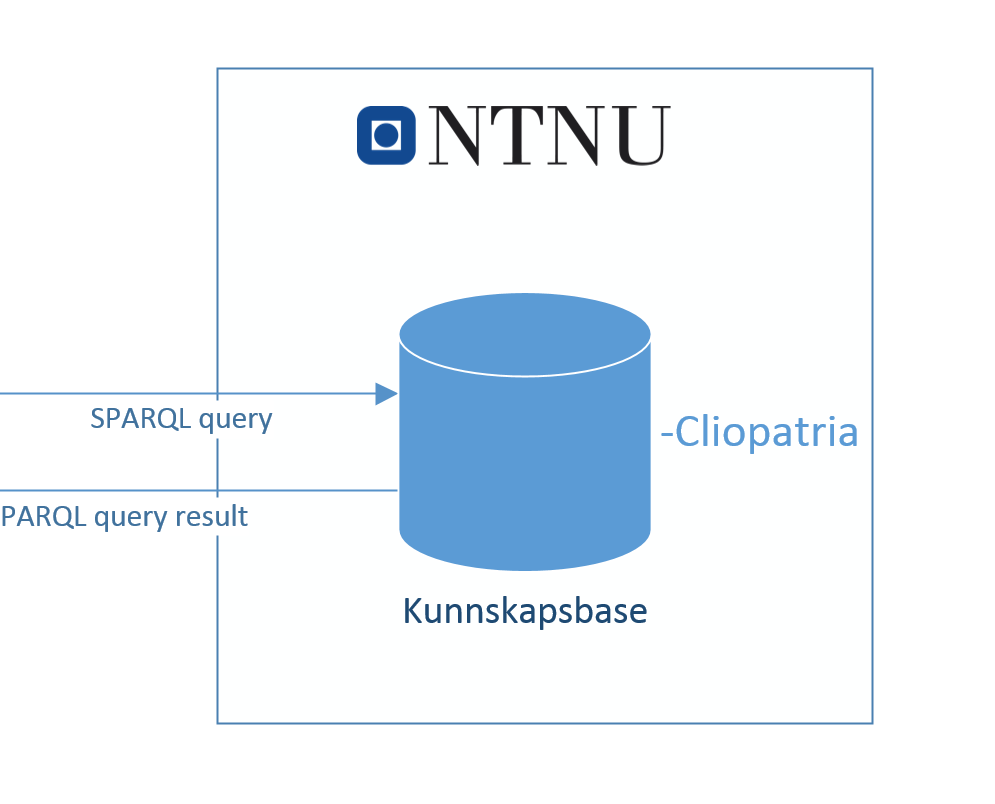
\includegraphics[width=10cm]{images/pille}
\caption{Azure-skytjeneste i SemLMG}
\label{fig:pille}
\end{figure}

\subsection{Webapplikasjonen}
\label{chap:webapp}
\subsubsection{Model-View-Controller arkitektonisk mønster}
\label{chap:mvc}
\gls{mvc} mønsteret er et arkitektonisk mønster brukt i programvareutvikling. Motivasjonen bak ligger i utvikling av grensesnitt. \gls{mvc} var en av de første tilnærmingene for å beskrive og implementere programvarekunstruksjoner i form av ansvarsområdet. \gls{mvc} mønsteret ble formulert av Trygve Reenskaug i 1970 og senere uttrykt som et generelt konsept i 1988 i en artikkel i The Journal of Object Techonology. \\
Målet med \gls{mvc} er å kunne skille på ansvaret til de ulike delene av systemet. For vedlikehold trenger ikke de ytre delene av systemet å vite noe om hvordan de indre delene ser ut, men heller andre veien. Kontrollerklasser vet alt om modellklasene, men ikke vice versa. Første tilknytningspunkt til brukeren vil være kontrolleren. Ansvaret til en kontrollerklasse vil være å sende meldinger til modellen om å oppdatere data. Dermed vil den sende meldinger til viewet om å oppdatere grensesnittet med riktig data. Modelklasser vil ha ansvaret for å modellere data og ha koblinger mot en database. Viewklasser har ansvar for de forskjellige grensesnittene og har ansvar for å oppdatere grensesnittene med riktig data.
Noe mer vanlig er å bruke en annen implementasjon av Model-view-conroller for å kunne binde flere modeller sammen og bruke i et view. Denne implementasjonen heter \gls{mvvm} og introduserer en ekstra ansvarsdel som heter viewmodel, som vist i figur \ref{fig:mvvm}. Dette er noe som ble brukt i utviklingen av webapplikasjonen da vi for eksempel hadde behov for å binde både en bruker med en kasuistikk og presentere data fra begge modellene. Her vil modellen endre seg med at viewmodelklassene vil binde sammen data fra modellene og grensesnittet for å kunne preseneteres for brukeren.
\begin{figure}[H]
\centering
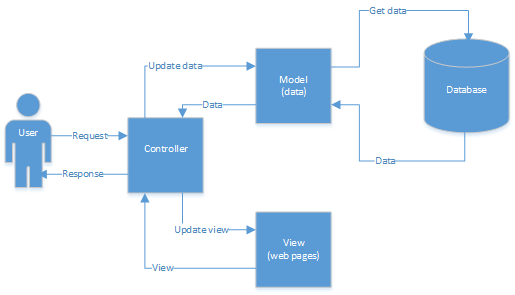
\includegraphics[width=14cm]{images/mvc}
\caption{MVC-mønsteret brukt i SemLMG}
\label{fig:mvc}
\end{figure}

\begin{figure}[H]
\centering
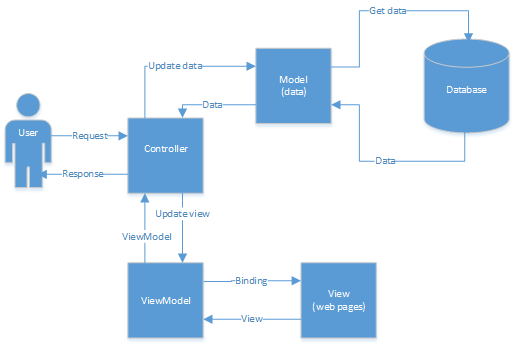
\includegraphics[width=14cm]{images/mvvm}
\caption{MVVM-mønsteret brukt i SemLMG}
\label{fig:mvvm}
\end{figure}

\newpage
\subsubsection{Entity framework}
For å enkelt kunne opprette, slette og endre databasen har vi valgt å bruke en objekt-relasjonsmapper kalt Entity framework. Dette eliminerer behovet for å skrive data-aksess kode mellom modellen og databasen. Entity framework viste seg å være et ganske kraftig verktøy for å opprette tabeller og databaser i det hele tatt. Etter å ha utforsket miljøet litt fant vi ut at vi kunne opprette hele databasebehovet vårt ved hjelp av code-first prinsipper med Entity framework. Code-first prinsippet går ut på at du ved annotasjoner i klassene dine bestemmer hva som er tabeller og hvilke datatyper som skal være attributter i tabellen i databasen. Når vi har satt opp alle klasser med datatyper er det bare å kjøre en migrasjon mot databasen og oppdatere den. Et slikt prinsipp viste seg å være kraftig når det gjelder konsistens. Hvis tabellene allerede finnes og modellene har endret seg, vil entity framework be deg om å kjøre en ny migrering slik at både kode og database har like forhold. Har du valgt code-first prinsipp så vil databasen da følge koden og ikke andre veien.
\begin{figure}[H]
\centering
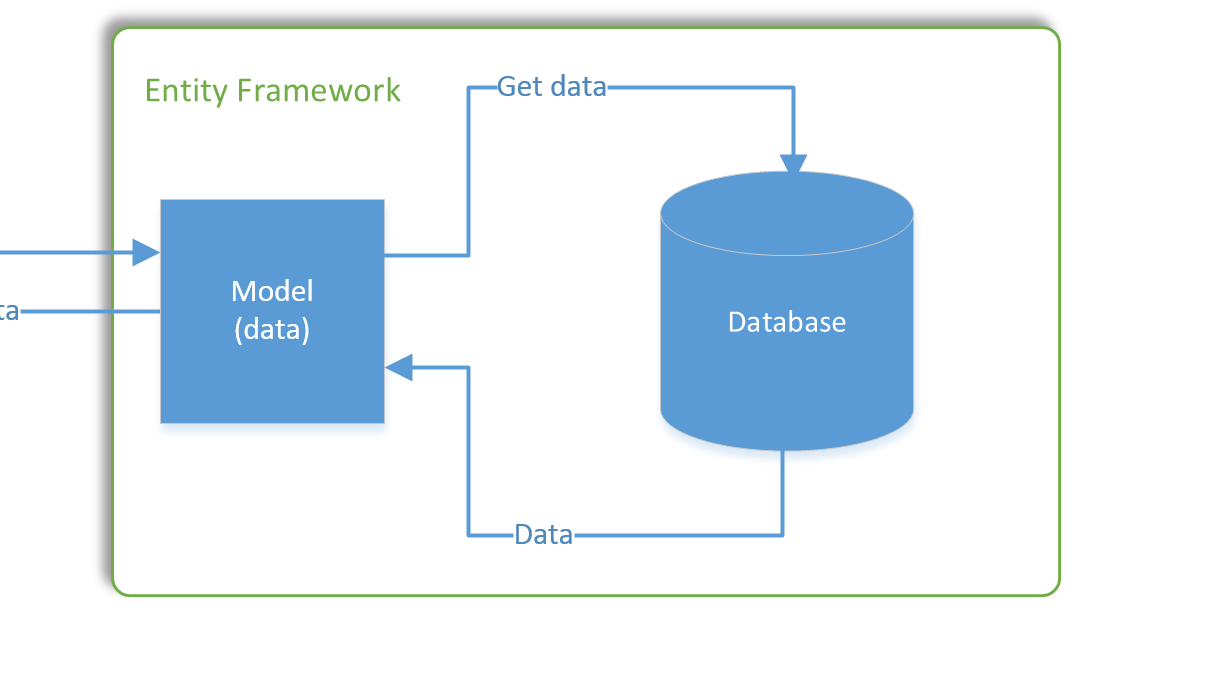
\includegraphics[width=14cm]{images/EntityFramework}
\caption{Entity framework kobling}
\label{fig:entityframework}
\end{figure}
\subsubsection{Samstemmingsverktøy}
Vår webapplikasjon gjenbrukte det nåværende samstemmingsverktøyet MedExt for å kunne trekke ut legemiddelinformasjon fra friteksten i kasuistikkene. Når brukeren var logget inn og ser kasuistikken må brukeren trykke ''Neste''-knappen for å gå videre i eksperimentet. Når denne klikkes gikk man videre og fikk se en liste over legemidler. Mellom disse vinduene var samstemmingsmodulen brukt. Samstemmingsmodulen tar inn fritekst, og gir ut en tekststreng i xml-format. Hvert enkelt legemiddel i denne tekststrenger blir da serialisert til legemiddelobjekter med tilhørende attributter som dose, doseringsenhet, frekvens og ATC-kode. 

\subsubsection{Design-klassemodellen}
For å få en forståelse for hvordan webapplikasjonen var bygd opp har vi modellert et klassediagram. Denne er representert i \ref{fig:classDiagram}. I modellen ser vi spor av MVVM-prinsippet. Vi har to base-klasser for kontroller- og viewmodel klasser. Model-klassene finner vi øver til høyre hvor vi finner Case,MedicalReview,CaseResult og User. Context-klassene er koblinger til database og fungrer som et knutepunkt mellom kontrollerne og modellene.
\begin{figure}[H]
\centering
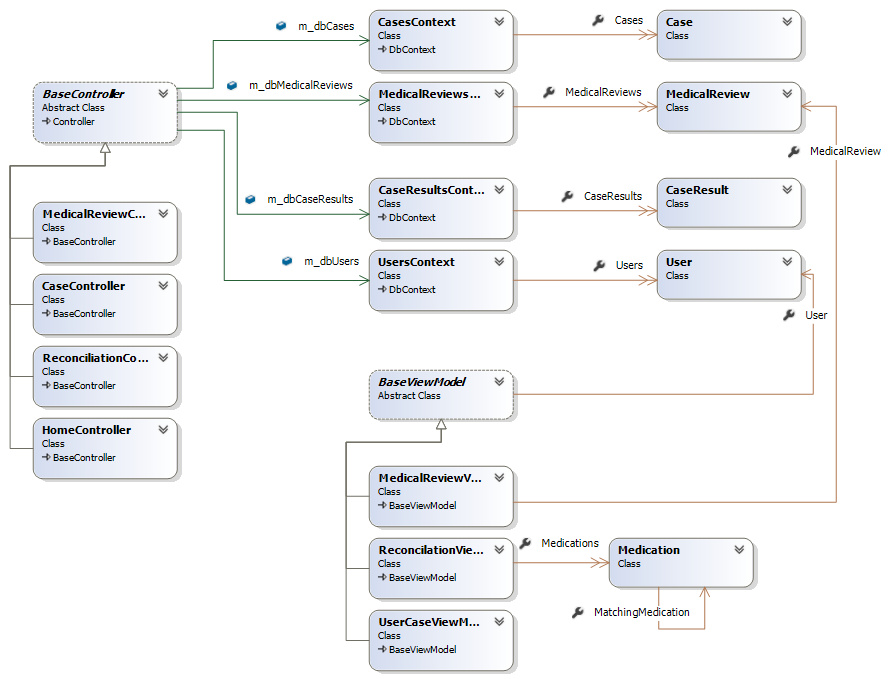
\includegraphics[width=14cm]{images/ClassDiagram.png}
\caption{Klassediagram for webgrensesnitt}
\label{fig:classDiagram}
\end{figure}

Vi ønsker å beskrive klassene dypere. Under vil vi ta for oss klassene som følger MVVM-prinsippet. Vi ønsker ikke å gå dypere inn i Context-klassene, da disse arver fra Entity Framework og krever bare at du spesifiserer hvilke modell-klasser som skal speiles med database. \\

\textbf{BaseController-klassehiarkiet} \\
I ASP.NET prosjekter blir klasser som har kontrollen på grensesnittet ofte referert til som kontroller-klasser. I figur \ref{fig:basecontroller} ser vi at vi hadde laget et grensesnitt med 4 forskjellige views. Dette var da de 4 sidene som skulle vises i webgrensesnittet. Hver av disse klassene arvet metoder fra BaseController for å kunne ha en felles måte å styre brukeren frem og tilbake mellom de forskjellige sidene. BaseController hadde også objekter for Context-klassene. Disse ble arvet på samme måte og betyr at på en hver side kunne vi gjøre endringer i databasen ved behov.
\begin{figure}[H]
\centering
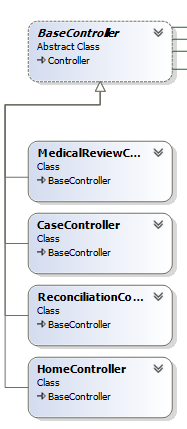
\includegraphics[width=4cm]{images/BaseController.png}
\caption{BaseController-klassehiarkiet}
\label{fig:basecontroller}
\end{figure}


\textbf{BaseViewModel-klassehiarkiet} 

Viewmodeller i vår webapplikasjon var designet til å kunne binde flere modeller sammen. Hos oss var vi alltid avhengig av at de forskjellige sidene hadde tilgang til en bruker samt en kasuistikk. Vi ser i figur \ref{fig:baseviewmodel} at navnene skal representere hva de inneholder. F.eks \textit{UserCaseViewModel} vil inneholde en binding mellom User og Case-klassene . 

Klassene var designet etter hvor de skal brukes. I vår webapplikasjon hadde vi en variabel som holdt styr på brukeren. Dette var en variabel som skal brukes på alle sider, og var dermed plassert i \textit{BaseViewModel} slik at alle viewmodellene kunne arve og bruke den. Det fantes naturligvis tilstander og hendelser som bare skulle skje på spesifikke sider, og disse var da plassert i de tilhørende viewmodellene. F.eks \textit{MedicalReviewViewModel} skulle ha holde styr på hvilke forsøkspersoner som skulle se forslag til tiltak eller ikke. Denne hadde da en boolsk variabel som ville endre seg etter hvilken bruker som var logget inn. Grensesnittet leste denne og endrer grensesnittet basert på verdien.
\begin{figure}[H]
\centering
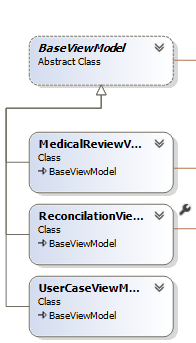
\includegraphics[width=4cm]{images/BaseViewModel.png}
\caption{BaseViewModel-klassehiarkiet}
\label{fig:baseviewmodel}
\end{figure}


\newpage
\textbf{Medication}

Når en samstemming ble gjort fikk vi legemidlene i et XML-format. Vi trengte \textit{Medication} klassen for å kunne hente ut attributter og sette de inn i et logisk objekt som vi kunne bruke senere. Medication klassen har dermed attributtene \textit{MedicationName},\textit{AtcCode},\textit{DosageValue},\textit{DosageUnit},\textit{Frequency}. Denne ble også brukt mot kunnskapsbasen for å kunne hente ut tiltak for hvert legemiddel.
\begin{figure}[H]
\centering
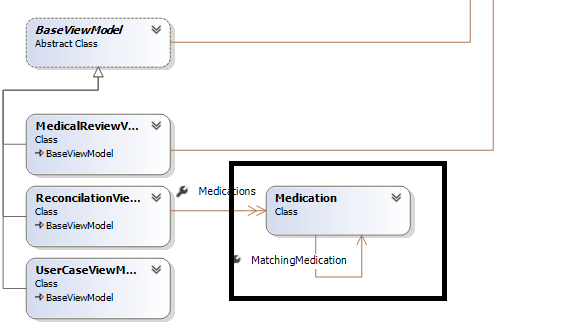
\includegraphics[width=10cm]{images/Medication.png}
\caption{Medication-klasse}
\label{fig:Medication}
\end{figure}


\textbf{Modell-klasser} 

Modell-klassene var basisen for hele prosjektet. Her har vi klassene \textit{User},\textit{Case},\textit{MedicalReview},\textit{CaseResult}. \textit{User} inneholder informasjon om en bruker som logger seg inn og gjennomfører eksperimentet.En hver \textit{User} er koblet sammen med en \textit{Case}, men denne koblingen ligger i \textit{Context-klassene}. \textit{Case} inneholder kasuistikk-teksten og er koblet sammen med \textit{CaseResult}. \textit{CaseResult} inneholder måling av tid på de forskjellige sidene i grensesnittet, dette er for å måle tiden det tar for brukere og utføre de forskjellige delene av eksperimentet. \textit{CaseResult} er koblet sammen med \textit{MedicalReview}. \textit{MedicalReview} inneholder alle tiltakene som blir skrevet inn av brukeren. \\
\begin{figure}[H]
\centering
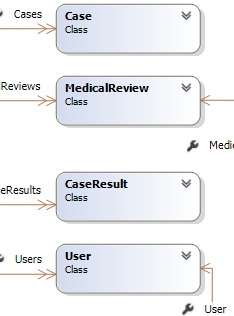
\includegraphics[width=4cm]{images/Models.png}
\caption{Modell-klasser}
\label{fig:models}
\end{figure}
Ved å lage webapplikasjonen på denne måten kunne vi enkelt styre grensesnittet, endre modeller og lagre ønsket informasjon. Vi kunne sjekke opp resultatet på en bruke etter den hadde utført eksperimentet og \textit{Context}-klassene hjalp oss med å lagre i databasen. Dette var hvor vi kunne se resultatene og hente dem ut for å videre analysere dem.


\subsection{Databasemodellen}
For å kunne ha en strukturert samling av relevant data, knyttet vi webapplikasjonen til en MySQL database. Denne databasen hadde som oppgave å bevare data om en bruker og brukerens kasuistikk samt resultater som ble lagret når webappliaksjonen ble brukt. Databasen var en relasjonsdatabase og følger de mest vanligste prinsippene for å kunne oppnå relasjoner mellom data. \\

I figur \ref{fig:umldiagramdatabase} er det modellert en UML representasjon av databasen. Videre ønsker vi å forklare nærmere hva hver tabell brukes til og trekke ut de viktigste attributtene i tabellen. *-symbolet etter et attributt betyr at dette attributtet er en primærnøkkel\footnote{En primærnøkkel er en unik verdi som vil identifisere en rad i tabellen} i tabellen. \underline{Understreket} attributt betyr at attributtet er en fremmednøkkel\footnote{ En fremmednøkkel er en referanseverdi til en rad i en annen tabell, dette er den mest vanligste metoden for å kunne ha relasjonsmønstre i en database} i tabellen.
%\end{description}
\begin{figure}[H]
\centering
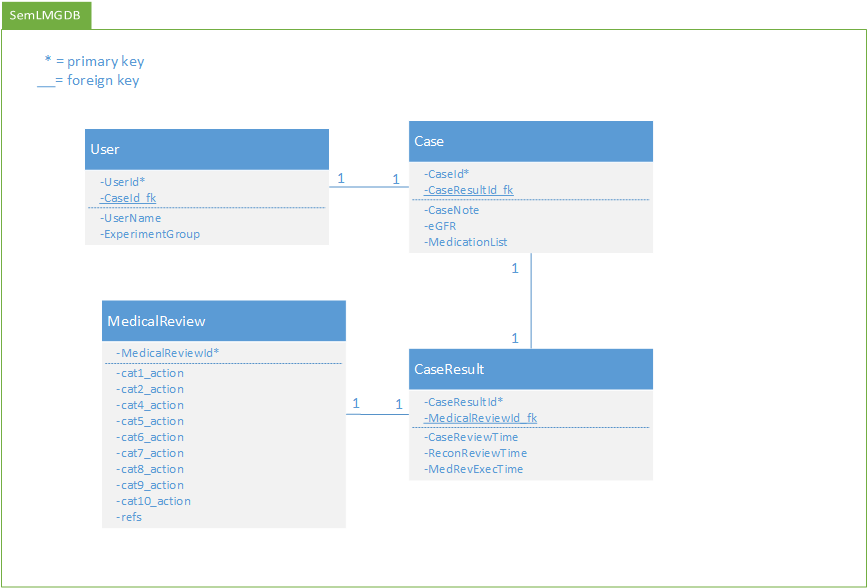
\includegraphics[width=16cm]{images/UMLDiagramDatabase.png}
\caption{UML diagram av database}
\label{fig:umldiagramdatabase}
\end{figure}
\label{chap:db}

\begin{description}
\newpage

\item[User]
var en tabell som skulle inneholde informasjon om en bruker.
\begin{description}
\item[UserName] var en streng som inneholdt brukernavnet til brukeren ved innlogging.
\item[ExperimentGroup] var et heltall som ville variere mellom 1 og 2. Verdien brukes til å skille mellom hvilke brukere som skulle få presentert en tiltaksliste eller ikke.
\end{description}

\item[Case] var en tabell skulle inneholde informasjon om en kasustikk. 
\begin{description}
\item[CaseNote] var en streng som ville inneholde hele teksten fra kasuistikken. Denne ville også være formatert i html-kodeformat for å kunne bli presentert i webgrensesnittet.
\item[eGFR] var et heltall som skulle bevare eGFR-verdien til kasuistikken. Denne ble brukt til å gjøre spørringer mot kunnskapsbasen.
\item[MedicationList] var en streng som inneholdt alle medisinene som ble nevnt i kasuistikken. Denne listen ble tolket av MedEXT og ble brukt til å gjøre spørringer mot kunnskapsbasen.
\end{description}

\item[CaseResult] var en tabell som skulle inneholde tidsmålinger på brukeren når brukeren navigerte seg frem og tilbake i applikasjonen. Webapplikasjonen hadde tre skjermbilder som det var interessant å måle tid på. Disse tre vinduene er lagrer tid en bruker i hvert vindu i tilsvarende \textbf{CaseReviewTime}, \textbf{ReconReviewTime} og \textbf{MedRevExecTime}.

\item[MedicalReview]  var en tabell som skulle inneholde informasjon om tiltakene som ble tatt og hvor brukeren klikker under LMG.
\begin{description}
\item[catX\_action] var en attributt som ble brukt for lagring av tiltak for kategorier. Disse tiltakene var det bruker som førte inn. Vi hadde 10 kategorier i LMG-skjemaet og dermed 10 attributter for hver kategori i databasen.
\item[refs] var en attributt som skulle lagre om en bruker hadde klikket på ''Bruk tiltak'' eller ''Les kilde''. Dette er en streng som blir tilføyd etterhvert som brukeren klikker på disse to knappene i grensesnittet.
\end{description}

\end{description}



\subsection{Kunnskapsbase}
\label{chap:kunnskapsbasedesign}
I kunnskapsbasen lå ontologien lagret. Til lagring av ontologien brukte vi Cliopatria, er en web server med et enkelt grensesnitt for å laste opp RDF filer.  Ontologien ble bygget ved bruk av verktøyet Protégé og lastet opp i Cliopatria, et triplestore basert på prolog. Protégé tilbyr et enkelt grensesnitt for å designe ontologien og populere den med individer(data). Cliopatria ga oss et web grensesnitt og et \gls{sparql} endpoint. Dette SPARQL-endpointet er det vi brukte for å sende spørringer fra prototypen ned til triplestoret. Spørringene har likheter med SQL, vi ''joiner'' data fra ulike deler av RDF-grafen.

Ontologien til prototypen er modellert i Figur \ref{fig:ont}. Modellen består av firkanter som representerer objekter, sirkler som representerer literaler og piler som representerer predikater. 

Under skal vi beskrive strukturen på ontologien i Figur \ref{fig:ont}:
\begin{description}

\item[Drug]
Et legemiddel, beskrevet med handelsnavnet. For eksempel Paracet som er handelsnavnet til medikamentet. I Paracet er det Paracetamol som er det aktive virkestoffet.

Predikater forbunnet med et Drug:
\begin{description}
\item[HasSubstance]
Et drug har predikat som binder det til et eller flere virkestoff. 
\end{description}


\item[Substance]
Substance er virkestoffet til legemiddelet. Det er virkestoffet som er den aktive ingrediensen i legemiddelet.

Predikater forbunnet med et Substance:
\begin{description}
\item[HasRecommandation]
Et Substance har predikat som binder det til et eller flere Recommandations. 
\end{description}


\item[Recommandation]
En Recommandation er anbefalingene til et virkestoff. Et virkestoff har ofte flere anbefalinger og i denne oppgaven har vi tatt hensyn til de anbefalingene som blir gitt ved nedsatt nyrefunksjon. 

Predikater forbunnet med en Recommandation:
\begin{description}
\item[LowerGFR og UpperGFR]
LowerGFR og UpperGFR er grensene for en Recommandation. En Recommandation er gyldig i et visst intervall  for eksempel ''GFR \textgreater 30 og GFR \textless 45''
\item[RecValue]
RecValue er verdien til en Recommandation. Den tekstlige anbefalingen hentet fra \url{www.uptodate.com}.
\item[RecType]
Vi skiller en Recommandation i to forskjellige kategorier ''Doseendring'' og ''Seponering''.
\item[HasSource]
Det er viktig at en Recommandation har en kilde. En Recommandation er koblet mot et Source-objekt ved hjelp av predikatet ''HasSource'' og Source er beskrevet under.
\item[RecID]
RecID er en unik id for anbefalingen. Brukes til å logge hvilke anbefalinger brukeren har brukt.
\item[StrengthOfRecommandation]
StrengthOfRecommandation brukes til å sortere listen over forslag som blir presentert for bruker. Vi sikrer at brukerene får den samme listen og at den blir lik hver gang. Dette parameteret kan brukes til å rangere hvor kritisk en anbefaling er slik at de viktigste anbefalingene kommer øverst.

\end{description}

\item[Source]
Source beskriver kilden til en Recommandation. Kilden er i denne oppgaven en URL til det aktuelle virkestoffet i \url{www.uptodate.com} og innholdet i hele anbefalingen hentet fra overskriften \textbf{Renal Impairment} kilden til en Recommandation. 
\begin{description}
\item[SourceURL]
URL direkte til der RecValue er hentet fra.
\item[SourceText]
Inneholder hele teksten der anbefalingene er hentet fra.
\end{description}
\end{description}

\begin{figure}[H]
\begin{center}
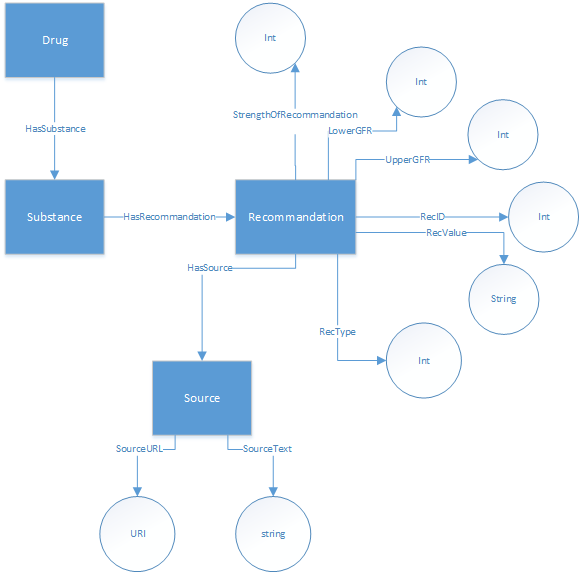
\includegraphics[width=12cm]{images/OntologiDiagram}
\caption{Ontologi modell}
\label{fig:ont}
\end{center}
\end{figure}

\subsection{Grensesnittet mot kunnskapsbasen}
Applikasjonen brukte \gls{sparql} endepunktet som Cliopatria eksponerte på web for å hente data fra ontologien. I \ref{lst:sparql} kan vi se hvordan spørringen er bygget opp og forklart under: 
\begin{description}
    \item[Linje  5 og 6] Her står de verdiene som ble hentet ut. Alle parameterene vi trengte til prototypen. Virkestoff label, recommandation verdi, strengthOfRecommandation, sourceURL, sourceText, recommandation type og Id, alle disse beskrevet i kapittel \ref{chap:kunnskapsbasedesign}.
    \item[Linje 7-17] Input fra systemet er markert i \{0\}, det er enten handelsnavnet til et medikament eller virkestoffet. Vi ser union av to sub-spørringer. Den første brukes hvis det er handelsnavnet av legemiddelet som sendes inn for å finne hvilket virkestoff som er knyttet til et legemiddel. Den andre sub-spørringen henter ut virkestoffet med samme navn som input.
    \item[Linje 19-24] Et virkestoff er knyttet til 0 - flere flere anbefalinger. Anbefalingene er er kun effektive i et intervall mellom to verdier av eGFR. Disse verdiene blir hentet ut fra anbefalingen og så filtrert ut slik at det er kun korrekt anbefaling som blir med lenger ned i spørringen.
    \item[Linje 26-33] Her hentet vi ut all data fra de forskjellige objektene. Navnet fra en ''substance'', forskjellige verdier fra en ''recommandation'' og URL/text fra kilden.
\end{description} 


\section{Demonstrasjon av prototype}
\ot{Husk å oppdatere bilder med nyeste versjon, se over teksten til hvert vindu slik at det passer}
\subsection{Innloggingsvindu}
Figur \ref{fig:demo1} viser forsiden til webapplikasjonen. Her kunne brukere logge inn med tilhørende brukernavn.
\begin{figure}[H]
\begin{center}
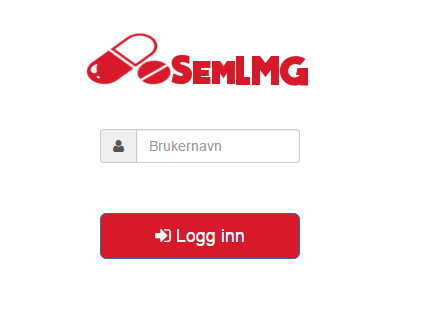
\includegraphics[width=8cm]{images/demoimages/1}
\caption{Innloggingsvindu}
\label{fig:demo1}
\end{center}
\end{figure}
Logoen øverst på siden ble fjernet når eksperimentet ble startet. Dette var for å ikke forvirre/forstyrre deltakeren med en logo som ikke har en funksjon.

\subsection{Kasuistikkvindu}
Figur \ref{fig:demo2} viser kasuistikkvinduet. Etter innlogging ble brukeren presentert for en pasientkasuistikk. Denne kasuistikken skulle brukeren lese og bli kjent med. Når brukeren var ferdig med å lese kasuistikken kunne han trykke ''Neste''.
\begin{figure}[H]
\begin{center}
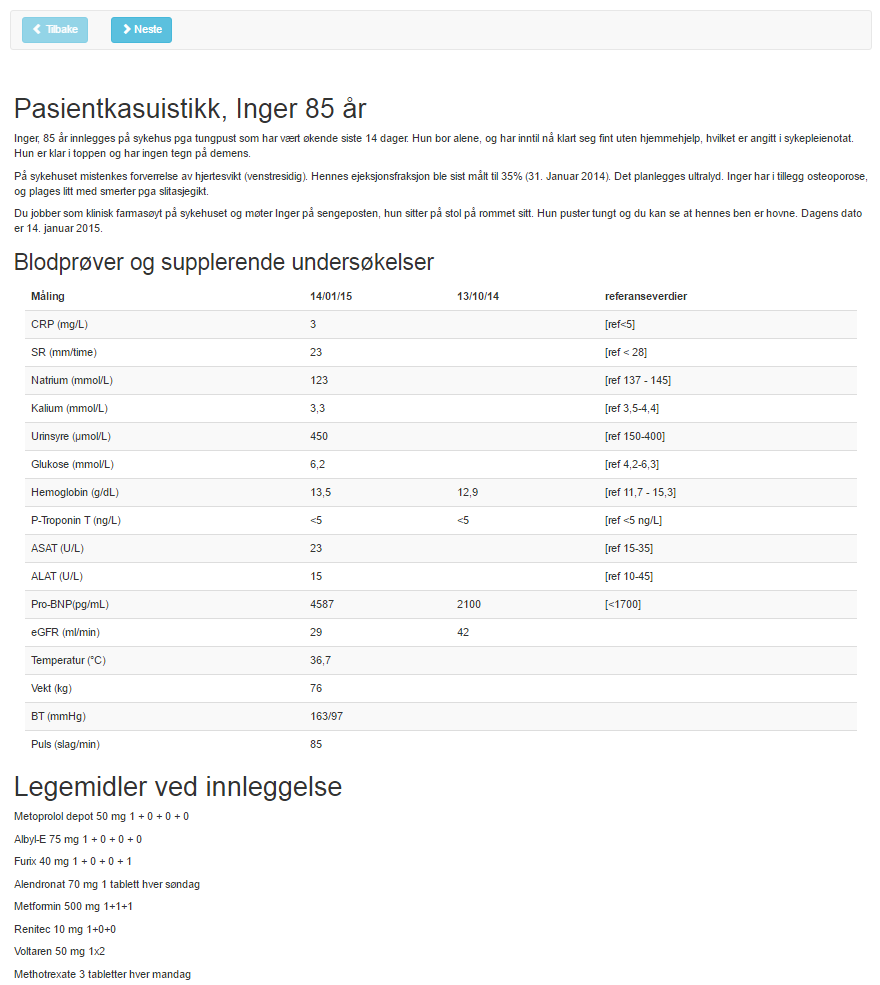
\includegraphics[width=14cm]{images/demoimages/2}
\caption{Kasuistikkvindu}
\label{fig:demo2}
\end{center}
\end{figure}

\newpage
\subsection{Vindu for legemidler i bruk}
Figur \ref{fig:demo3} viser legemidler i bruk vinduet. Dette var et vindu hvor brukeren skulle observere at en LiB-liste ble laget fra pasientkasuistikken. Når brukeren var ferdig med å observere listen kunne de trykke ''Neste''.
\begin{figure}[H]
\begin{center}
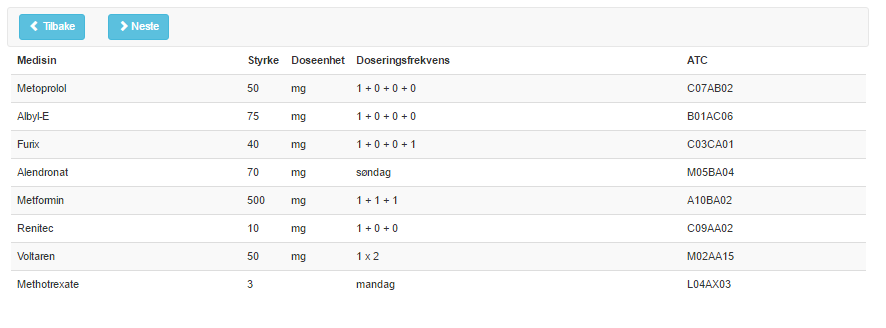
\includegraphics[width=18cm]{images/demoimages/3}
\caption{LiB-vindu}
\label{fig:demo3}
\end{center}
\end{figure}

\newpage
\subsection{Legemiddelgjennomgangvindu}
Figur \ref{fig:demo4} viser legemiddelgjennomgangen som brukeren skulle utføre. Vinduet bestod av et lignende skjema som kliniske farmasøyter bruker i dag. Dette er et skjema som blir fylt ut når farmasøyter finner forslag til tiltak under en legemiddelgjennomgang. I figur \ref{fig:demo4} hadde brukeren muligheten til å se forslag til tiltak under en bestemt kategori. Dette er kategorien som vil inneholde tiltak for nedsatt nyre og leverfunksjon. Vinduet består også av den samstemte legemiddellisten (til høyre) og kasuistikken (nederst).
\begin{figure}[H]
\begin{center}
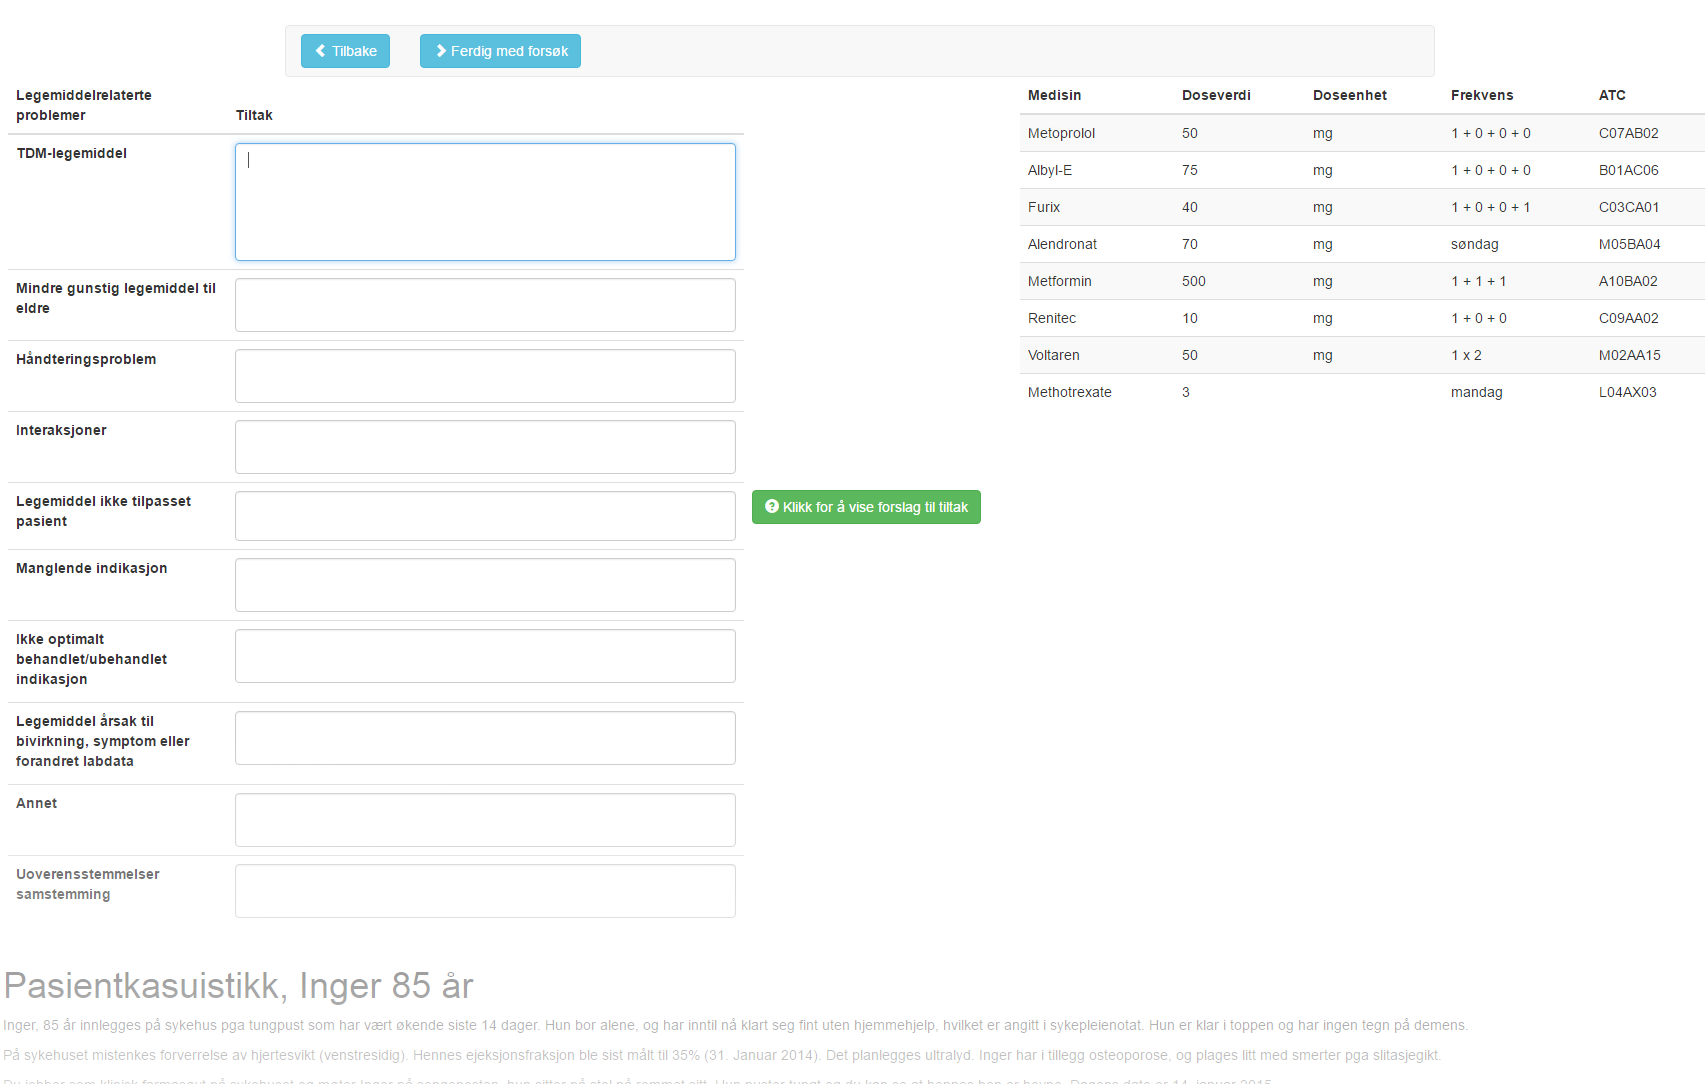
\includegraphics[width=18cm]{images/demoimages/4}
\caption{LMG-vindu}
\label{fig:demo4}
\end{center}
\end{figure}
\newpage
 Hvis brukeren trykte på knappen ''Klikk for å vise forslag til tiltak'' ville en liste med forslag dukke opp under legemiddellisten (høyre). I figur \ref{fig:demo5} ser vi at grensesnittet har forandret seg til hvordan det så ut når en bruker ønsket å se listen.
\begin{figure}[H]
\begin{center}
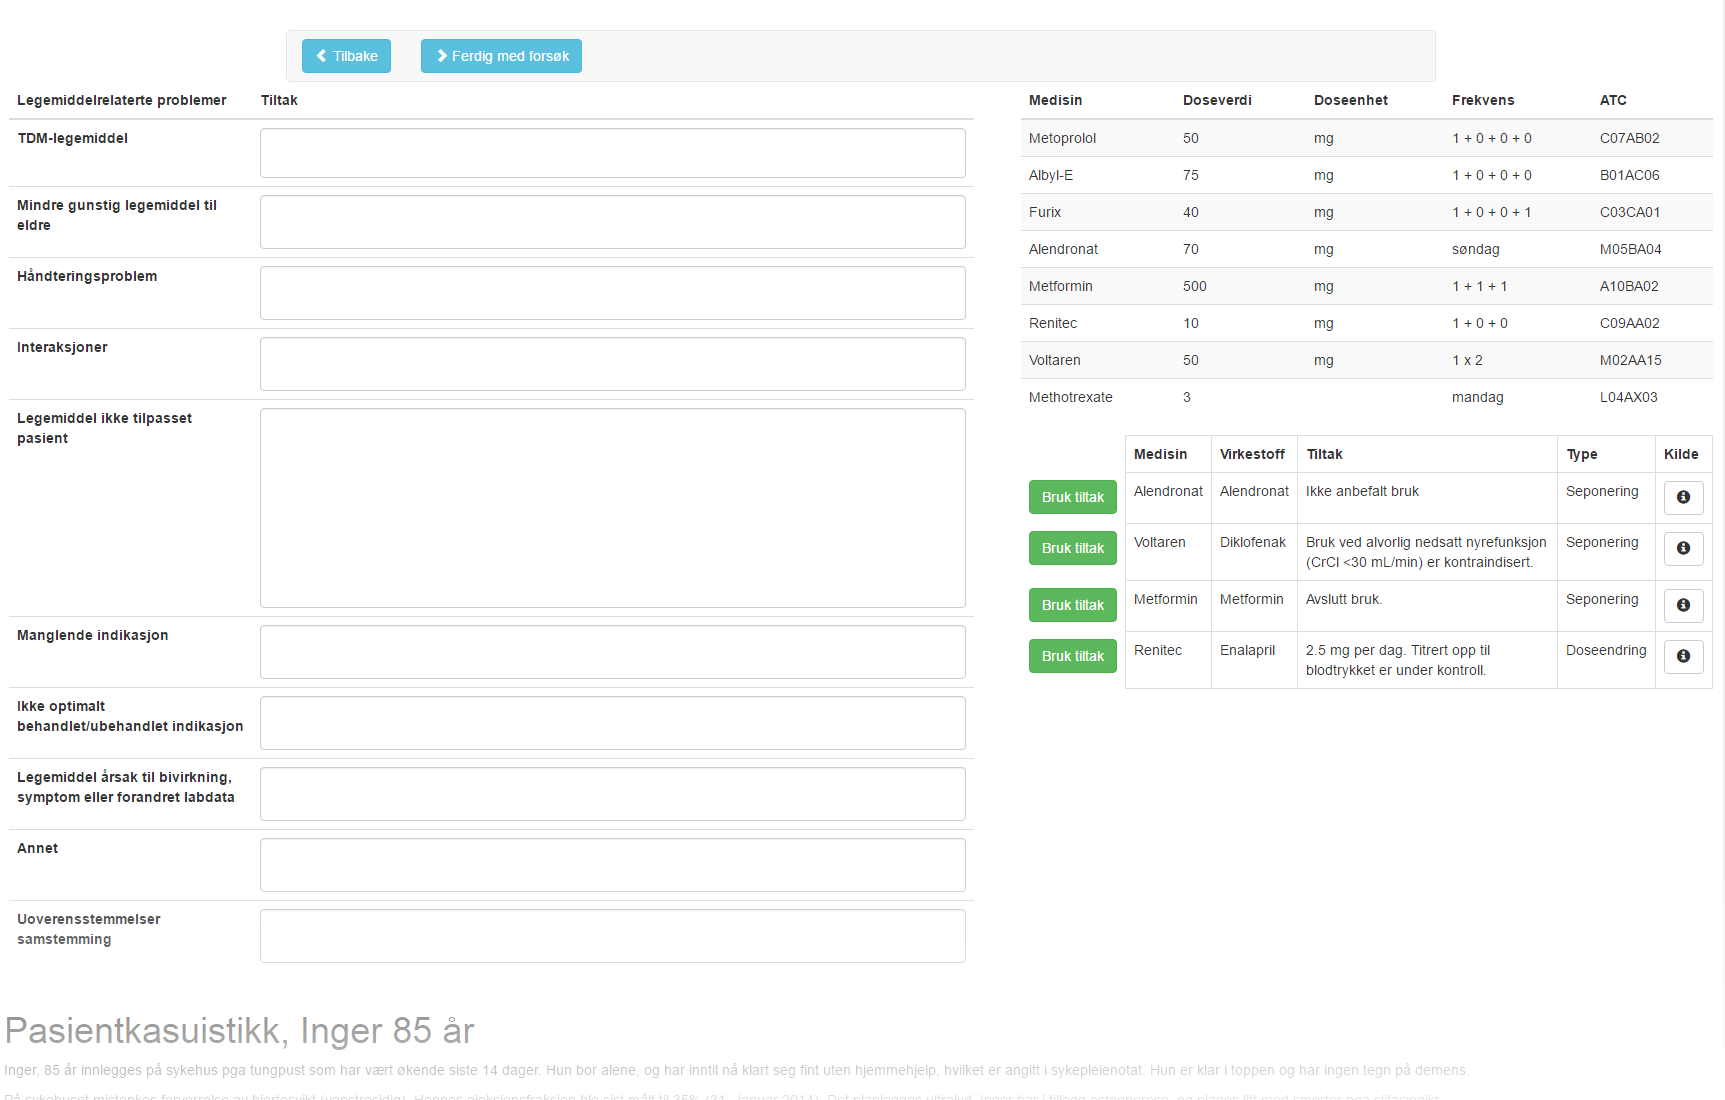
\includegraphics[width=18cm]{images/demoimages/5}
\caption{LMG-vindu med forslag til tiltak}
\label{fig:demo5}
\end{center}
\end{figure}
\newpage
 I denne listen kunne brukeren velge å bruke tiltak. Disse tiltakene ble da automatisk skrevet inn i tiltaksfeltet i skjemaet. Dette kan vi se i figur \ref{fig:demo6}. Når brukeren følte seg ferdig med LMG-skjemaet kunne man presse ''Ferdig med forsøk''.
\begin{figure}[H]
\begin{center}
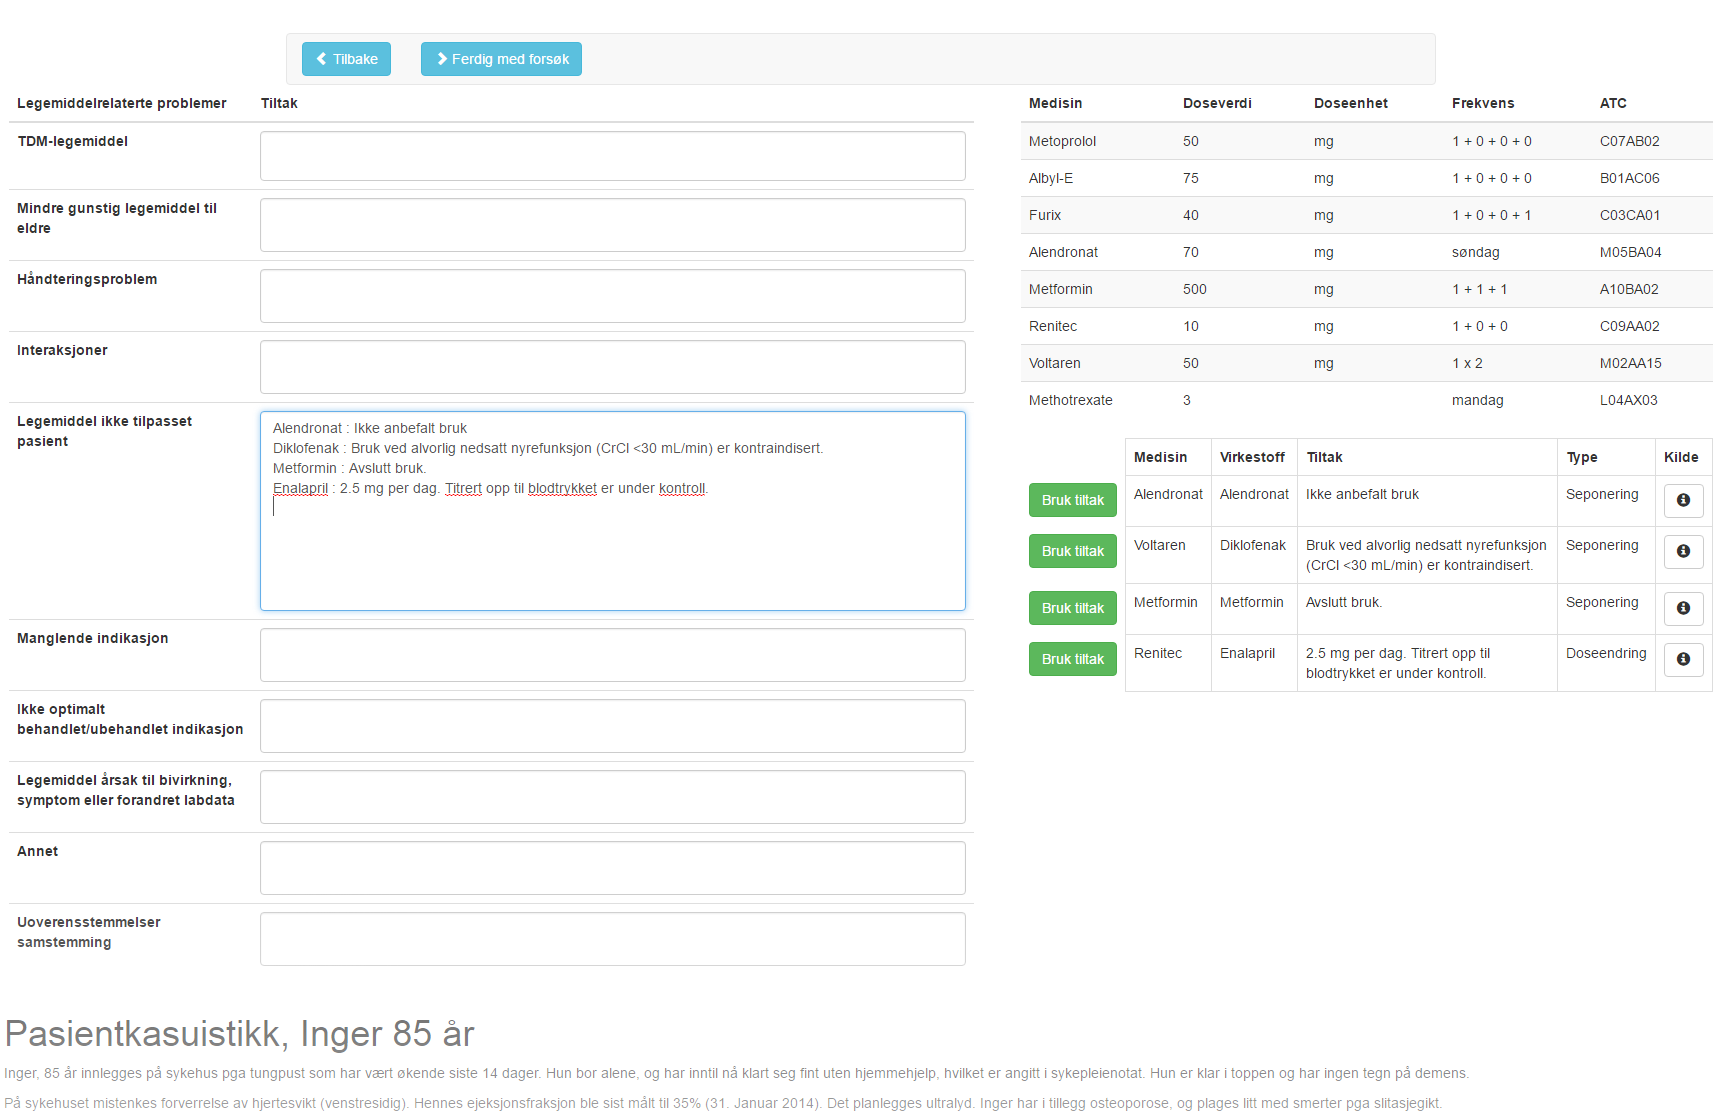
\includegraphics[width=18cm]{images/demoimages/6}
\caption{LMG-vindu med brukte tiltak}
\label{fig:demo6}
\end{center}
\end{figure}

\newpage



\section{Gjennomføring av eksperiment}
\label{chap:gjenomf_eksperiment}
\subsection{Rekruttering av deltagere}
Ved hjelp av våre biveildere ved Sykehusapoteket i Trondheim rekrutterte vi kliniske farmasøyter til å delta i eksperimentet. 30 kliniske farmasøyter ble kontaktet. Disse jobbet primært ved Sykehusapoteket i Trondheim, med noen innslag av kliniske farmasøyter ved sykehusapoteker i Nord-Trøndelag samt Møre og Romsdal. Ut av disse 30 svarte 10 at de ønsket å delta i eksperimentet. Av disse 10 var 4 kliniske farmasøyter ved Sykehusapoteket i Trondheim. 

For å rekruttere kliniske farmasøyter til utføring av et fokusgruppeintervju, måtte vi ta utgangspunkt i de som allerede har sagt seg villig til å delta i eksperimentet. Siden fokusgruppeintervjuet tok utgangspunkt i bruk av støttesystem som SemLMG, ville rekruttering av kliniske farmasøyter som ikke deltok på eksperimentet være ut av kontekst. De fire kliniske farmasøytene som jobbet i Trondheim ble kontaktet, da de resterende syv av praktiske hensyn ikke var mulig å rekruttere.
//For further notice: hvor mange av disse var villige til å delta i fokusgruppe?

\subsection{Informasjon for gjennomføring}
I forkant fikk deltagerne en introduksjon til SemLMG og hvordan de skulle bruke det for å gjennomføre eksperimentet. Denne informasjonen sendte vi ut sammen med brukernavnene til hver enkelt deltager samt tidsfrist og annen praktisk informasjon. Informasjonsskrivet er i sin helhet vedlagt i \ref{vedlegg:informasjonsskriv}.

\subsection{Spørreskjema}
Et spørreskjema ble utviklet. Denne var basert på spørsmål utviklet av en klinisk farmasøyt som tok utgangspunkt i pasientkasuistikkene i SemLMG. Halvparten av spørsmålene var rettet mot foreslåtte tiltak og den andre halvparten på legemiddelrelatert kompetanse. Den andre halvdelen av spørsmålene gikk på dypere kompetansene rundt legemidlene. De fleste spørsmålene hadde flere svaralternativ som den kliniske farmasøyten sto for. Videre ble en fasit utviklet, som vi brukte for å sette en poengsum for antall riktige i spørreundersøkelsen.

Det var flere valgmuligheter når det kom til å lage spørreundersøkelse på nett. Opprinnelig ble Questback brukt. Questback brukes mye i næringslivet, og siden våre biveiledere hadde tilgang til verktøyet virket dette fornuftig\ot{Er dette relevant?}. Etterhvert skulle det vise seg at Questback var vanskelig å konfigurere, i tillegg til at vi ikke hadde tilgang selv. Derfor valgte vi å ta i bruk Google Forms, noe som vi har hatt kjennskap til før. Spørreundersøkelsen er tilgjengelig i \ref{vedlegg:magne} og \ref{vedlegg:inger}.

\subsection{Pretest}
Før eksperimentet kunne starte var det behov for å utføre en pretest. Dette var en prosess vi sammen med veiledere ønsket å utføre for å kunne oppdage og rette feil. Målet var å forbedre prototypen og spørreskjema hvis det var nødvendig. Pretesten ble utført på hovedveileder og biveiledere. \\
Et annet alternativ vi hadde for å kunne få en enda bedre evaluering av forsøket var å ha en pre-pretest samt en pretest. For å kunne gjennomføre dette måtte vi tatt ut to-tre personer fra deltakergruppen og brukt disse til pretest. En pre-pretest kunne da ha blitt utført med hovedveileder og biveiledere, mens pretesten hadde vært faktiske deltakere. Det var planlagt at en person måtte bruke to til tre dager på å utføre eksperimentet. På lik linje ønsket vi at pretestere også skulle få samme antall dager på å utføre en pretest. Dette vil bety at vi ville utsatt datoen for innsamling av resultater fra eksperiment med to-tre dager. Det ble derfor besluttet at eksperimentet var så godt som det kunne bli på den tiden vi hadde, og at en pretest på tre personer var godt nok for å gjøre nødvendige endringer. \\
Vi fikk gode resultater av pretesten. Noen tilbakemeldinger gikk på endringer i grensesnitt, mens andre gikk direkte på kasuistikken. Generelt fikk vi positive tilbakemeldinger.

\subsubsection{Personvern}



\subsection{Fokusgruppeintervju}


\chapter{Resultat og analyse}
\label{chap:res_og_anal}
\section{Resultat av eksperiment}
\subsection{Tidsmålinger}
\subsection{Legemiddelgjennomgangskjema}
\subsection{Kompetansespørsmål}

\section{Analyse av resultater}
\label{chap:resanal_analyseavresultater}
\subsection{Tidsmålinger}
\subsection{Legemiddelgjennomgangskjema}
\subsection{Kompetansespørsmål}



\chapter{Diskusjon}
\section{Gyldighet av resultatene}



\chapter{Konklusjon}
\input{chapters/konklusjon}


\chapter{Videre arbeid}
\input{chapters/videre_arbeid}


\bibliographystyle{plainnat}
\bibliography{bib/bibl}




\pagenumbering{gobble}
\newgeometry{right=1cm,left=1cm,top=0cm,bottom=0cm}
\titleformat{\chapter}[hang] 
{\normalfont\huge\bfseries}{\chaptertitlename\ \thechapter:}{1em}{} 

\begin{appendices}


\chapter{Sparql Query}\label{vedlegg:sparqlquery}

\begin{lstlisting}[captionpos=b, caption=SPARQL query, label=lst:sparql,
   basicstyle=\tiny,frame=single]
PREFIX    rdf:<http://www.w3.org/1999/02/22-rdf-syntax-ns#>
PREFIX   rdfs:<http://www.w3.org/2000/01/rdf-schema#>
PREFIX master:<http://www.semanticweb.org/espenrh/ontologies/2016/2/untitled-ontology-3#>

SELECT ?label ?val ?strength ?sourceURL 
?sourceText ?recType ?id WHERE {  
{  select ?substance where {
     ?drug master:hasSubstance ?substance . 
     ?drug rdfs:label ?label . 
     filter(lcase(str(?label)) = lcase(str("{0}")))
  }}
    UNION 
{  select ?substance where {
     ?substance rdf:type master:Substance .
     ?substance rdfs:label ?label .
      filter(lcase(str(?label)) = lcase(str("{0}")))
  }}
  
    ?substance master:hasRecommandation ?rec .
    ?rec master:upperGFR ?upperGFR .
    ?rec master:lowerGFR ?lowerGFR .

    filter (?upperGFR > {1})                       
    filter(?lowerGFR <= {1}) 

    ?substance rdfs:label ?label .
    ?rec master:recValue ?val .
    ?rec master:strengthOfRecommandation ?strength .
    ?rec master:hasSource ?source .
    ?rec master:recType ?recType .
    ?rec master:recID ?id .
    ?source master:sourceURL ?sourceURL .
    ?source master:sourceText ?sourceText 
   }
\end{lstlisting}



\chapter{Milepæleplan}\label{vedlegg:milep}
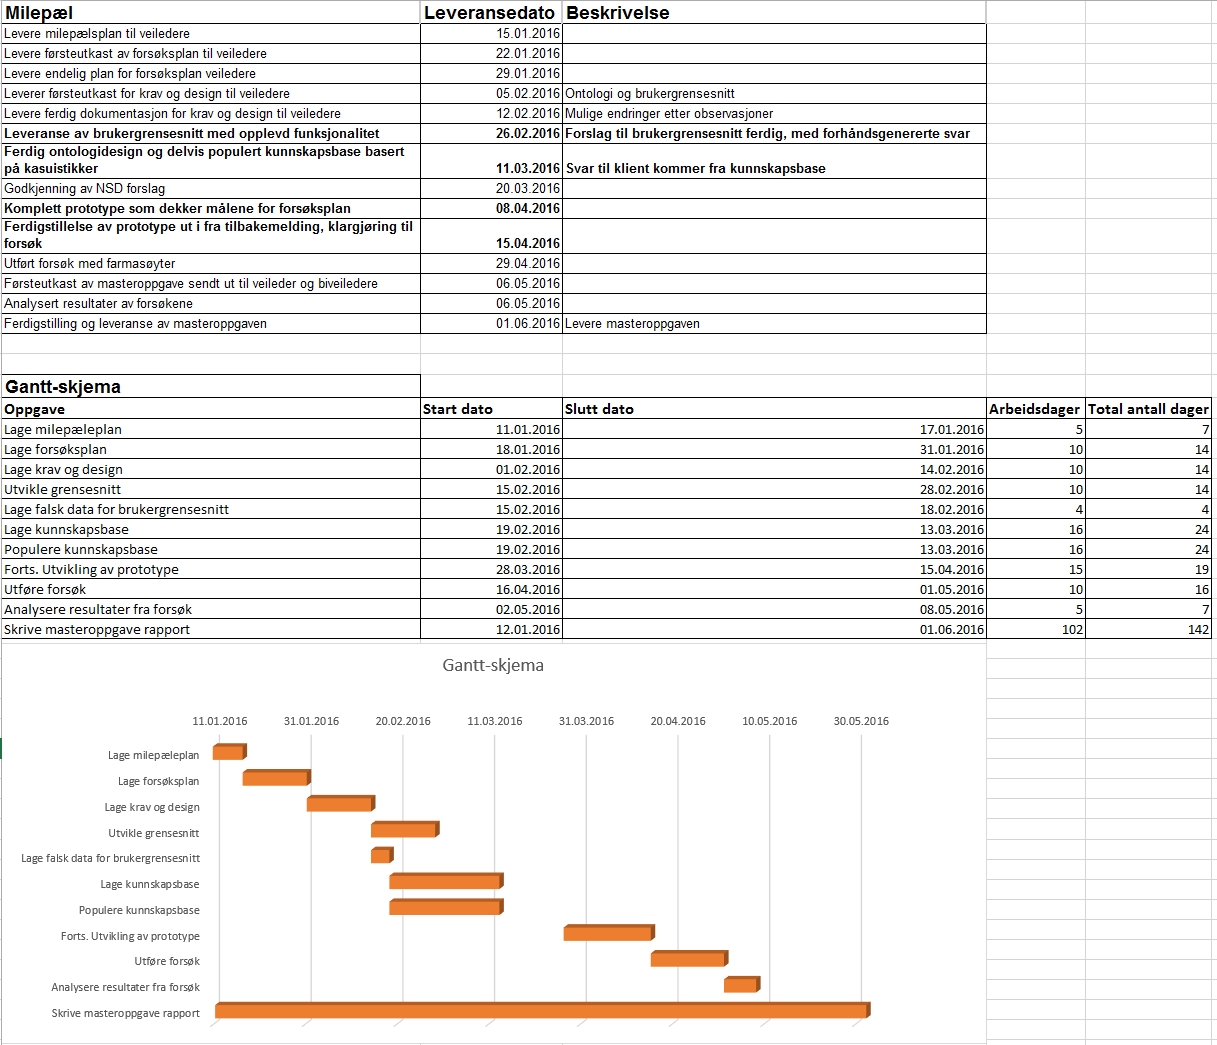
\includegraphics[angle=90,height=18cm]{images/Fremdriftsplan}

\chapter{Kasuistikk - Inger} \label{vedlegg:kasus_inger}
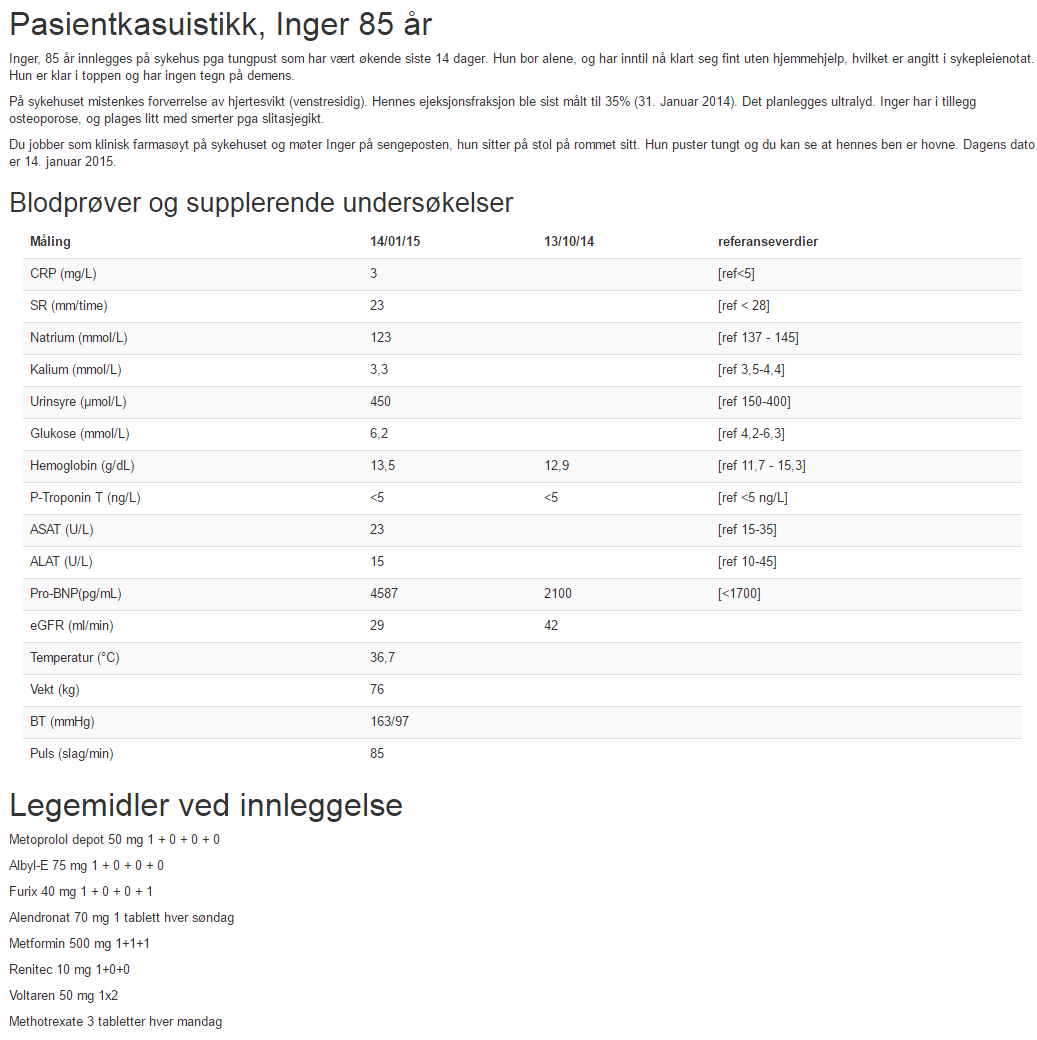
\includegraphics[height=15cm]{images/Kasuistikk_inger}

\chapter{Kasuistikk - Magne} \label{vedlegg:kasus_magne}
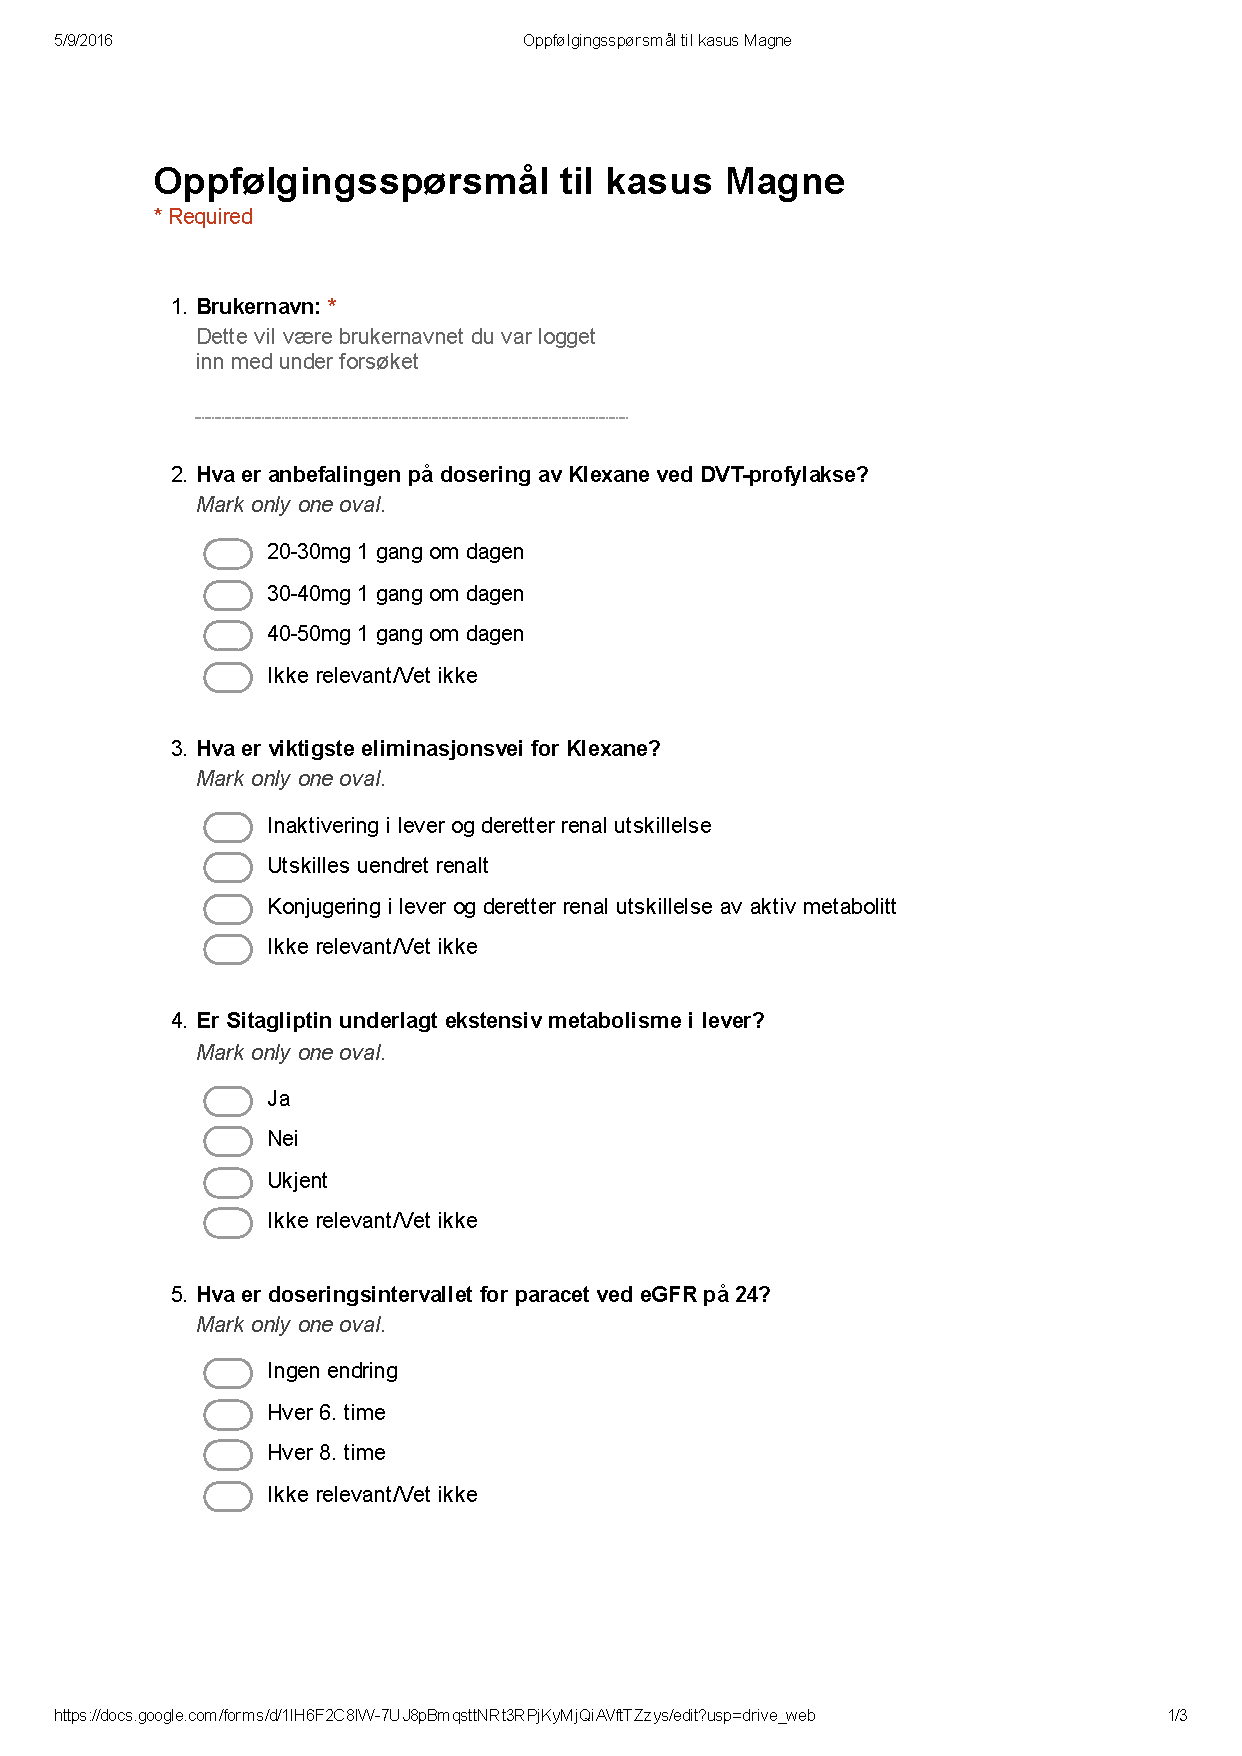
\includepdf[pages={1,2}]{pdf/magne}


\chapter{Informasjonsskriv til deltagere}\label{vedlegg:informasjonsskriv}
\begin{adjustwidth}{2cm}{2cm}
Takk for at du er villig til å delta i forsøket vårt.

Vi er tre IT-studenter ved Institutt for Datateknikk og Informasjonsvitenskap ved NTNU som arbeider med vår avsluttende masteroppgave om datastøttet legemiddelgjennomgang.

I forsøket skal du bruke et elektronisk LMG-skjema som likner på det du er vant til. Du blir presentert for to pasientkasus, og for ett av kasusene vil systemet presentere mulig relevante tiltak eller råd. Testen kunne vært gjennomført på papir, men det gjøres på nett av praktiske hensyn. Etter hvert kasus får du noen spørsmål hvor vi undersøker effekten av datastøtten. Alle deltakere får oppgaver og kasus som likner mye på hverandre, så vær snill å ikke samarbeide eller røpe innholdet før svarfristen er gått ut mandag 9. mai kl. 12:00

Undersøkelsen er anonym. Vi samler ingen personlig informasjon og bruker individuavhengige identifikatorer. Vi trenger dermed ingen godkjenning fra NSD (eller REK).

Svarene fra spørreundersøkelsen vil vurderes av en farmasøyt.


Veiledning i gjennomføring av forsøket:

Forsøket går ut på å lese en kasuistikk, se en samstemt legemiddeloversikt, fylle ut skjemaet med identifiserte LRP og til slutt svare på noen spørsmål.
Du skal gjøre dette to ganger, for to forskjellige pasientkasus.

Innholdet er fordelt på flere nettsider, og du kan bestandig navigere fram og tilbake mellom disse med knappene øverst til venstre («forrige» og «neste»).
(I et virkelig system ville all informasjonen være på ett skjermbilde, men det var upraktisk i et nettbasert eksperiment.)

Når du er ferdig med et pasientkasuset blir du ledet videre til en spørreundersøkelse.
Etter du har gjort LMG og svart på spørreundersøkelse med første brukernavn går du videre til brukkernavn nr 2.
Hele forsøket er forventet å ta ca. 30 minutter.
Tilgang til forsøk:
Brukernavn 1. : storekorn
Brukernavn 2. : finekorn

Trykk på denne lenken for å starte forsøket: http://semlmg.azurewebsites.net

Har du spørsmål?

Kontakt:
Navn: Espen Rise Halstensen, Frode Rennemo og Håvard Moås.
Mail: helsemaster@list.stud.ntnu.no
Tlf: 97 97 45 51


Hovedveileder:
Navn: Øystein Nytrø
Mail: oeystein.nytroe@gmail.com

Biveiledere:
Navn: Ingvild Klevan
Mail: Ingvild.Klevan@sykehusapoteket.no

Navn: Janne Sund
Mail: Janne.Sund@sykehusapoteket.no


 \end{adjustwidth} 

\chapter{Spørreundersøkelse - Magne kasuistikk}\label{vedlegg:magne}
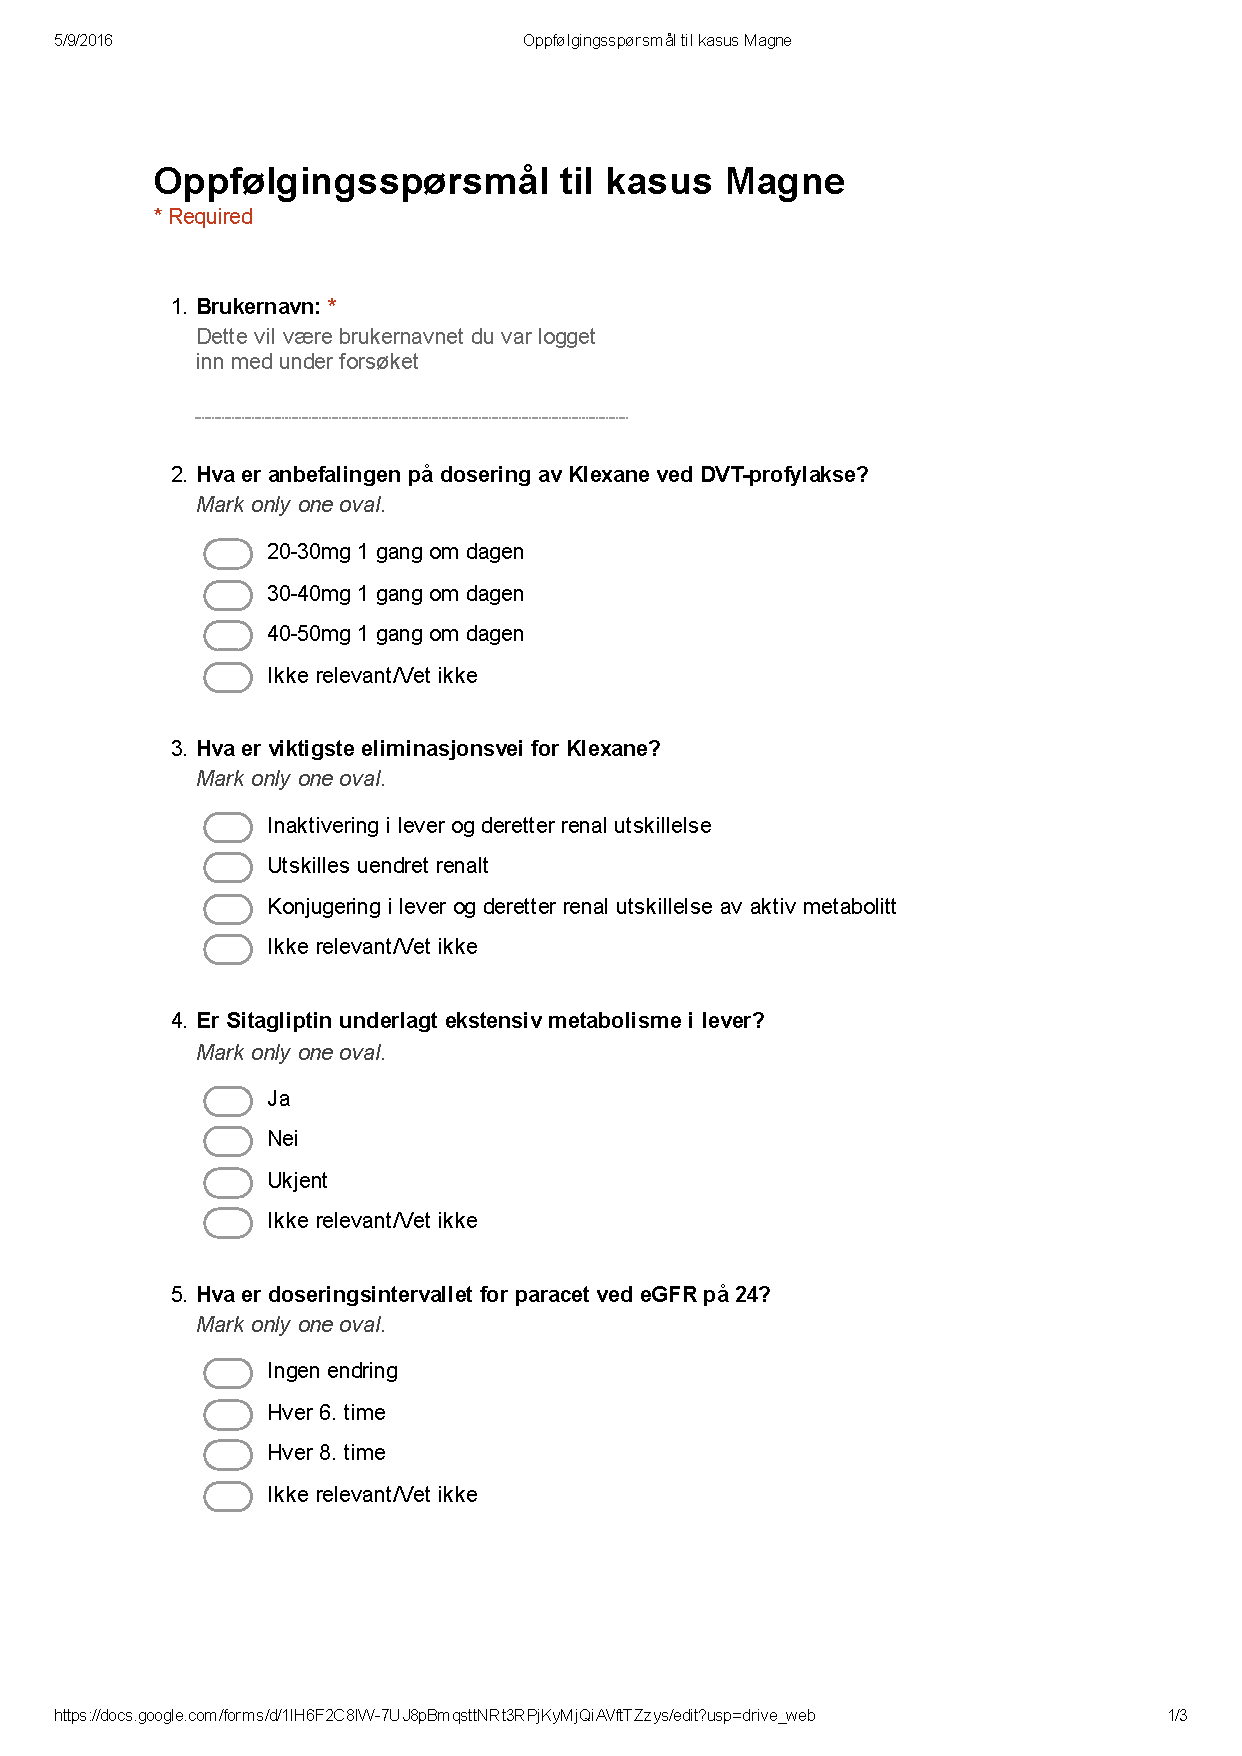
\includepdf[pages={1,2}]{pdf/magne}

\chapter{Spørreundersøkelse - Inger kasuistikk}\label{vedlegg:inger}
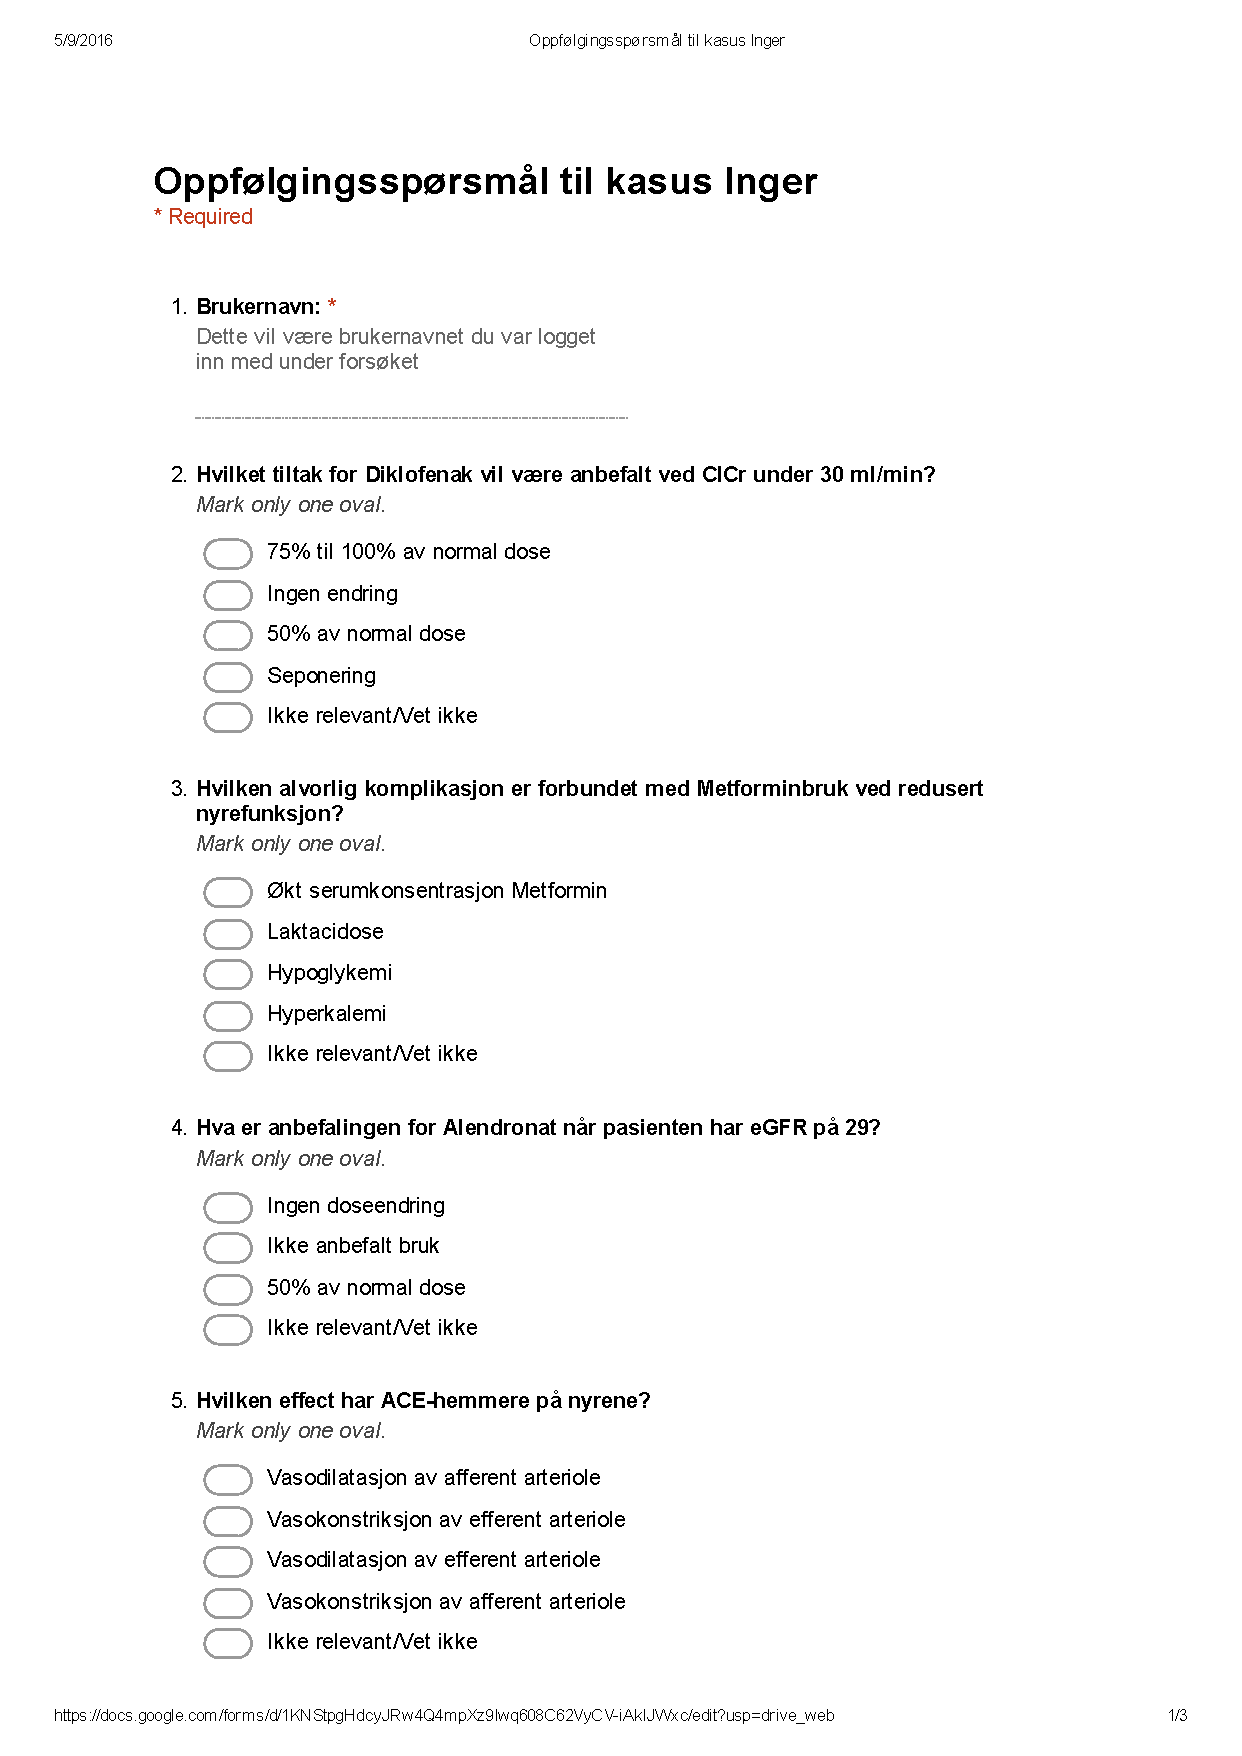
\includepdf[pages={1,2}]{pdf/inger}



\end{appendices}
\restoregeometry


\end{document}
